% Webinar 5 of the Idiot Brain series (Armenian): chapter 6, "Personality: a testing concept".
% Build from the repo root through the shared queue (never run lualatex directly):
%     python 02_idiot_brain/slides/common/build_deck.py webinar05            one pass, ~3 min
%     python 02_idiot_brain/slides/common/build_deck.py webinar05 --full     latexmk until stable, ~10-17 min
% Needs the art first: uv run 02_idiot_brain/slides/common/build_art.py
% Speaker notes: NOTES.md (by frame number and title). ~95 min talk incl. a 5 min break.
\documentclass[aspectratio=169,11pt]{beamer}
% =====================================================================
%  The Idiot Brain webinars - shared Beamer preamble (the banner look)
% ---------------------------------------------------------------------
%  Usage (in slides/webinarNN/webinarNN.tex):
%      \documentclass[aspectratio=169,11pt]{beamer}
%      % =====================================================================
%  The Idiot Brain webinars - shared Beamer preamble (the banner look)
% ---------------------------------------------------------------------
%  Usage (in slides/webinarNN/webinarNN.tex):
%      \documentclass[aspectratio=169,11pt]{beamer}
%      % =====================================================================
%  The Idiot Brain webinars - shared Beamer preamble (the banner look)
% ---------------------------------------------------------------------
%  Usage (in slides/webinarNN/webinarNN.tex):
%      \documentclass[aspectratio=169,11pt]{beamer}
%      \input{../common/preamble.tex}
%  Build from the deck folder:  latexmk -lualatex -outdir=build webinarNN.tex
%  Art (emoji, mascot moods, title banner) comes from common/build_art.py.
%
%  All styling lives here, so decks only hold content. Palette and fonts
%  are the banner's (banner/build_banner.py): plum text on cream, pastel
%  accents, Mardoto for text, Glazz for big titles, Twemoji icons and
%  the pink brain mascot (DECISIONS.md #4-#6).
% =====================================================================

% ---------------------------------------------------------------------
% Fonts (LuaLaTeX + fontspec), shared with the banner
% ---------------------------------------------------------------------
\usepackage{fontspec}
\tracinglostchars=3 % a glyph missing from a font stops the build instead of printing nothing
\defaultfontfeatures{Ligatures=TeX}
\def\idiotfontdir{../../banner/assets/fonts/}
\setsansfont{Mardoto}[Path=\idiotfontdir, Extension=.ttf, UprightFont=*-Regular, BoldFont=*-Bold]
\setmainfont{Mardoto}[Path=\idiotfontdir, Extension=.ttf, UprightFont=*-Regular, BoldFont=*-Bold]
\newfontfamily\mediumfont{Mardoto-Medium}[Path=\idiotfontdir, Extension=.ttf]
\newfontfamily\blackfont{Mardoto-Black}[Path=\idiotfontdir, Extension=.ttf]
\newfontfamily\titlefont{GlazzArm-Regular}[Path=\idiotfontdir, Extension=.ttf] % Armenian letters only
\newfontfamily\handfont{Ink Free} % Windows font with Armenian; speech bubbles only
% Mardoto has no italic: emphasis is medium weight in the accent colour instead.
\renewcommand{\emph}[1]{{\mediumfont\color{plum}#1}}
% No hyphenation: split words are hard to read on a shared screen.
\hyphenpenalty=10000
\exhyphenpenalty=10000

% ---------------------------------------------------------------------
% Packages
% ---------------------------------------------------------------------
\usepackage{graphicx}
\usepackage{booktabs}
\usepackage[most]{tcolorbox}
\usepackage{tikz}
\usetikzlibrary{arrows.meta, positioning, calc, shapes.geometric, shapes.callouts, shapes.misc,
  decorations.pathmorphing, decorations.pathreplacing, backgrounds, fit, patterns.meta}
\usepackage{pgfplots}
\pgfplotsset{compat=1.18}
\usepgfplotslibrary{fillbetween}
\graphicspath{{../common/art/}{images/}}

% ---------------------------------------------------------------------
% Colours: the banner palette. Charts with 3+ series use the Armenian
% flag colours (amRed / amBlue / amOrange).
% ---------------------------------------------------------------------
\definecolor{plum}{HTML}{4A2340}
\definecolor{brainpink}{HTML}{F7A8C4}
\definecolor{fold}{HTML}{E57FA6}
\definecolor{cream}{HTML}{FFF6EC}
\definecolor{cardwhite}{HTML}{FFFDF9}
\definecolor{peach}{HTML}{FFD9C2}
\definecolor{lavender}{HTML}{D9C8F5}
\definecolor{mint}{HTML}{B5E8D5}
\definecolor{butter}{HTML}{FFE8A3}
\definecolor{blush}{HTML}{FF8FA8}
\definecolor{amRed}{HTML}{D90012}
\definecolor{amBlue}{HTML}{0033A0}
\definecolor{amOrange}{HTML}{F2A800}
% darker partners for text on cream
\colorlet{mintdark}{mint!45!black!80!green}
\definecolor{mintdark}{HTML}{2E7D62}
\definecolor{lavenderdark}{HTML}{5B3FA0}
\definecolor{peachdark}{HTML}{B5532A}
\definecolor{pinkdark}{HTML}{C2185B}
% names used by the figure files
\colorlet{ink}{plum}
\colorlet{paper}{cream}
\colorlet{mist}{lavender!40!cream}
\definecolor{night}{HTML}{2B2150}
\colorlet{softgray}{plum!60!cream}
% accent of the current part; \partaccent{<colour>} switches it
\colorlet{accent}{butter}
\newcommand{\partaccent}[1]{\colorlet{accent}{#1}}

% ---------------------------------------------------------------------
% Art: \emoji, \mascot (pages of common/art/*.pdf, see build_art.py)
% ---------------------------------------------------------------------
\makeatletter
\newcommand{\artpage}[3]{\expandafter\def\csname idiot@art@#1@#2\endcsname{#3}}
\input{../common/art/art_index.tex}
\newcommand{\idiot@art}[3]{% kind, name, size options
  \ifcsname idiot@art@#1@#2\endcsname
    \includegraphics[#3, page=\csname idiot@art@#1@#2\endcsname]{#1.pdf}%
  \else
    \PackageError{idiot}{Unknown #1 '#2'; add it to build_art.py and rebuild the art}{}%
  \fi}
% \emoji[<height>]{name}: inline icon, sits on the text baseline like a letter
\newcommand{\emoji}[2][1.15em]{\raisebox{-0.2em}{\idiot@art{emoji}{#2}{height=#1}}}
% \bigemoji[<height>]{name}: no baseline shift, for TikZ nodes and big pictures
\newcommand{\bigemoji}[2][1.5cm]{\idiot@art{emoji}{#2}{height=#1}}
% \mascot[<width>]{mood}: panic, happy, scared, sleepy, sick, confused, smug, hungry, thinking
\newcommand{\mascot}[2][2.6cm]{\idiot@art{mascot}{#2}{width=#1}}
\makeatother
% the older figure files place the mascot with \pic{noggin=<mood>}
\tikzset{pics/noggin/.style={code={\node[inner sep=0, transform shape] {\mascot[2.7cm]{#1}};}}}

% ---------------------------------------------------------------------
% Beamer look
% ---------------------------------------------------------------------
\setbeamertemplate{navigation symbols}{}
\setbeamercolor{normal text}{fg=plum, bg=cream}
\setbeamercolor{structure}{fg=plum}
\setbeamercolor{alerted text}{fg=pinkdark}
\setbeamerfont{alerted text}{series=\bfseries}
\setbeamercolor{frametitle}{fg=plum}
\setbeamersize{text margin left=9mm, text margin right=9mm}
\setbeamertemplate{frame begin}{\raggedright} % justified Armenian leaves big gaps

% cream paper with the banner's faint dot grid
\setbeamertemplate{background}{%
  \begin{tikzpicture}
    \fill[cream] (0,0) rectangle (\paperwidth,\paperheight);
    \fill[pattern={Dots[distance=4.4mm, radius=0.28mm]}, pattern color=plum!9!cream]
      (0,0) rectangle (\paperwidth,\paperheight);
  \end{tikzpicture}}

% topic pill, top right of every frame: set by \topic (emoji + short name)
\def\idiottopicemoji{}
\def\idiottopicname{}
\newcommand{\idiotpill}[3][cardwhite]{% fill, emoji, text
  \tikz[baseline=(p.base)]{\node[fill=#1, draw=plum, line width=0.7pt, rounded corners=2.6mm,
      inner xsep=2.2mm, inner ysep=1.1mm, font=\mediumfont\footnotesize, text=plum] (p)
      {\ifx\relax#2\relax\else\emoji[1.05em]{#2}\hspace{1.2mm}\fi#3};
    \begin{scope}[on background layer]
      \fill[plum, rounded corners=2.6mm] ([xshift=0.7mm, yshift=-0.7mm]p.south west) rectangle ([xshift=0.7mm, yshift=-0.7mm]p.north east);
    \end{scope}}}
% \chip{emoji}{text}: inline sticker label, same as the banner's topic chips
\newcommand{\chip}[3][cardwhite]{\idiotpill[#1]{#2}{#3}}

\setbeamertemplate{frametitle}{%
  \vskip 3.5mm
  \begin{minipage}[t]{0.66\paperwidth}
    \raggedright{\blackfont\fontsize{17.5}{20.5}\selectfont\insertframetitle}\par
    \vskip 1.3mm
    \tikz\fill[accent, rounded corners=0.6mm] (0,0) rectangle (1.5cm,1.1mm);
  \end{minipage}%
  \hfill
  \ifx\idiottopicname\empty\else
    \raisebox{-1mm}{\idiotpill{\idiottopicemoji}{\idiottopicname}}%
  \fi
  \vskip 1mm}

\setbeamertemplate{footline}{%
  \hbox to \paperwidth{\hskip 9mm
    {\mediumfont\fontsize{7}{8}\selectfont\color{plum!55!cream}Ապուշ ուղեղը · \insertshorttitle}\hfill
    {\blackfont\fontsize{8}{9}\selectfont\color{plum!70!cream}\insertframenumber}\hskip 9mm}
  \vskip 3mm}

\setbeamertemplate{itemize item}{\tikz[baseline=-0.65ex]\draw[plum, fill=accent, line width=0.6pt] (0,0) circle (0.95mm);}
\setbeamertemplate{itemize subitem}{\tikz[baseline=-0.65ex]\fill[plum!70] (0,0) circle (0.6mm);}
\setbeamertemplate{enumerate item}{\tikz[baseline=(n.base)]\node[fill=accent, draw=plum, line width=0.6pt,
  circle, inner sep=0.5mm, minimum size=4.2mm, font=\blackfont\scriptsize] (n) {\insertenumlabel};}
\setlength{\leftmargini}{5mm}
\setbeamertemplate{itemize/enumerate body begin}{\setlength{\itemsep}{1.6mm}}
\setbeamertemplate{itemize/enumerate subbody begin}{\setlength{\itemsep}{0.6mm}\small}

% ---------------------------------------------------------------------
% Structure: parts (full-colour openers) and topics (book sections)
% ---------------------------------------------------------------------
% \topic{<emoji>}{<short name>}: starts a book section; the pill shows on every following frame
\newcommand{\topic}[2]{\subsection{#2}\gdef\idiottopicemoji{#1}\gdef\idiottopicname{#2}}
\newcommand{\notopic}{\gdef\idiottopicemoji{}\gdef\idiottopicname{}}

% \partopener{<label>}{<title>}{<subtitle>}{<mood>}{<colour>}
\newcommand{\partopener}[5]{%
  \section{#2}\notopic\partaccent{#5}%
  \begin{frame}[plain]
    \begin{tikzpicture}[remember picture, overlay]
      \fill[#5] (current page.south west) rectangle (current page.north east);
      \fill[pattern={Dots[distance=4.4mm, radius=0.28mm]}, pattern color=plum!12!#5]
        (current page.south west) rectangle (current page.north east);
      \fill[cardwhite, opacity=0.45] ([xshift=-3.3cm, yshift=-0.2cm]current page.east) circle (3.1cm);
      \node[anchor=north west, inner sep=0] at ([xshift=10mm, yshift=-12mm]current page.north west)
        {\idiotpill{}{#1}};
      \node[anchor=west, text=plum, align=left, text width=9.2cm, inner sep=0]
        (t) at ([xshift=10mm, yshift=5mm]current page.west)
        {\titlefont\fontsize{38}{40}\selectfont #2};
      \node[anchor=north west, text=plum, text width=9.2cm, inner sep=0, align=left]
        at ([yshift=-5mm]t.south west) {\mediumfont\large #3};
      \node at ([xshift=-3.3cm, yshift=-0.2cm]current page.east) {\mascot[4.6cm]{#4}};
    \end{tikzpicture}
  \end{frame}}

% \topicopener{<emoji>}{<short name>}{<book's section title>}{<what it is about>}{<mood>}
\newcommand{\topicopener}[5]{%
  \topic{#1}{#2}%
  \begin{frame}[plain]
    \begin{tikzpicture}[remember picture, overlay]
      \fill[accent!55!cream] (current page.south west) rectangle (current page.north east);
      \fill[pattern={Dots[distance=4.4mm, radius=0.28mm]}, pattern color=plum!10!accent!55!cream]
        (current page.south west) rectangle (current page.north east);
      \node[anchor=north west, inner sep=0] at ([xshift=10mm, yshift=-12mm]current page.north west)
        {\idiotpill{#1}{#2}};
      \node[anchor=west, text=plum, text width=9.6cm, align=left, inner sep=0]
        (t) at ([xshift=10mm, yshift=6mm]current page.west)
        {\blackfont\fontsize{24}{28}\selectfont «#3»};
      \node[anchor=north west, text=plum, text width=9.6cm, align=left, inner sep=0]
        at ([yshift=-4mm]t.south west) {\mediumfont\large #4};
      \node at ([xshift=-3.0cm, yshift=-0.4cm]current page.east) {\mascot[4.2cm]{#5}};
      \node[rotate=-12] at ([xshift=-1.4cm, yshift=2.3cm]current page.east) {\bigemoji[1.5cm]{#1}};
    \end{tikzpicture}
  \end{frame}}

% ---------------------------------------------------------------------
% Boxes (sticker style: plum outline + hard plum shadow, like the banner)
% ---------------------------------------------------------------------
\tcbset{
  sticker/.style={enhanced, arc=3mm, boxrule=0.9pt, colframe=plum, colback=cardwhite, halign=left,
    left=3mm, right=3mm, top=2mm, bottom=2mm, fontupper=\normalsize, coltext=plum,
    shadow={1.1mm}{-1.1mm}{0mm}{fill=plum}},
  tagged/.style={sticker, colback=#1!45!cream, colbacktitle=#1, coltitle=plum,
    fonttitle=\blackfont\footnotesize, top=3mm,
    attach boxed title to top left={xshift=4mm, yshift*=-2.4mm},
    boxed title style={arc=2.2mm, boxrule=0.9pt, colframe=plum, left=1.5mm, right=1.5mm, top=0.6mm, bottom=0.6mm}},
}
\newtcolorbox{card}[1][]{sticker, #1}
\newtcolorbox{tryit}[1][]{tagged=mint, title={\emoji[1em]{testtube}\ Փորձիր հիմա}, #1}
\newtcolorbox{poll}[1][]{tagged=butter, title={\emoji[1em]{hand}\ Հարցում}, #1}
\newtcolorbox{chatbox}[1][]{tagged=lavender, title={\emoji[1em]{speech}\ Գրիր չաթում}, #1}
\newtcolorbox{scienceupdate}[1][]{tagged=peach, fontupper=\small, title={\emoji[1em]{microscope}\ Գիտությունն այսօր}, #1}
\newtcolorbox{bookquote}[1][]{sticker, colback=cardwhite, fontupper=\mediumfont, left=4mm,
  borderline west={1.4mm}{0pt}{accent},
  before upper={{\blackfont\footnotesize\emoji[1em]{book}\ Բըրնեթը գրում է}\par\smallskip}, #1}

% Brain.exe-style popup window: \begin{popup}{<window title>} ... \end{popup}
\newcommand{\winbuttons}{%
  \tikz[baseline=-0.6ex, line width=0.6pt]{
    \foreach \i/\f in {0/cardwhite, 1/cardwhite, 2/blush}{
      \filldraw[fill=\f, draw=plum, rounded corners=0.6mm] (\i*4.3mm,-1.6mm) rectangle ++(3.3mm,3.3mm);}
    \draw[plum] (0.8mm,-0.8mm) -- (2.5mm,-0.8mm);
    \draw[plum] (5.1mm,-0.8mm) rectangle (6.8mm,0.9mm);
    \draw[plum] (9.4mm,-0.9mm) -- (11.1mm,0.8mm) (9.4mm,0.8mm) -- (11.1mm,-0.9mm);}}
\newtcolorbox{popup}[2][]{sticker, colback=cardwhite, colbacktitle=brainpink, coltitle=plum,
  fonttitle=\blackfont\small, title={\emoji[1.1em]{warning}\hspace{1.5mm}#2\hfill\winbuttons},
  titlerule=0.9pt, toptitle=0.8mm, bottomtitle=0.8mm, #1}

% Myth or fact: \mythorfact{<statement>}{<verdict>}{<colour>}{<explanation>}; verdict shows on slide 2
\newcommand{\mythorfact}[4]{%
  \begin{center}
  \begin{tikzpicture}
    \node[draw=plum, line width=0.9pt, fill=cardwhite, rounded corners=4mm, inner xsep=8mm, inner ysep=6mm,
          text width=10cm, align=center, font=\blackfont\Large, text=plum] (mf) {«#1»};
    \begin{scope}[on background layer]
      \fill[plum, rounded corners=4mm] ([xshift=1.2mm, yshift=-1.2mm]mf.south west) rectangle ([xshift=1.2mm, yshift=-1.2mm]mf.north east);
    \end{scope}
    \node[anchor=west] at ([xshift=6mm]mf.north west) {\idiotpill[butter]{question}{Առասպել, թե՞ փաստ}};
    \onslide<2->{\node[draw=#3, text=#3, line width=2pt, rounded corners=2mm, rotate=-10, font=\blackfont\LARGE,
      inner sep=4pt, fill=cardwhite] at ([xshift=-8mm, yshift=1mm]mf.south east) {#2};}
  \end{tikzpicture}
  \end{center}
  \onslide<2->{#4}}

% Big question with the confused mascot: \bigquestion{<question>}{<small line>}
\newcommand{\bigquestion}[2]{%
  \vfill
  \begin{center}
  \begin{tikzpicture}
    \node[text width=9.6cm, align=center, font=\blackfont\fontsize{24}{29}\selectfont, text=plum] (q) {#1};
    \node[below=4mm of q, text width=9.6cm, align=center, font=\mediumfont\large, text=softgray] {#2};
    \node[anchor=east] at ([xshift=-2mm]q.west) {\mascot[2.6cm]{confused}};
  \end{tikzpicture}
  \end{center}
  \vfill}

% Small source line at the bottom of a frame: \source{Loftus & Palmer, 1974}
\newcommand{\source}[1]{%
  \begin{tikzpicture}[remember picture, overlay]
    \node[anchor=south east, font=\fontsize{6.5}{7.5}\selectfont, text=plum!60!cream, inner sep=0]
      at ([xshift=-17mm, yshift=3.4mm]current page.south east) {Աղբյուր՝ #1};
  \end{tikzpicture}}

% Speech bubbles (handwritten) and the overlay helper for TikZ:
% \node[visible on=<2->] ... keeps the layout but hides the node until slide 2.
\tikzset{
  say/.style={rectangle callout, draw=plum, line width=0.8pt, fill=cardwhite, rounded corners=3pt,
    inner sep=4pt, align=center, font=\handfont\normalsize, text=plum},
  think/.style={cloud callout, cloud puffs=12, draw=plum, line width=0.8pt, fill=cardwhite,
    inner sep=2pt, align=center, font=\handfont\normalsize, text=plum},
  % boxes for diagrams drawn directly in a frame: a style with #1 cannot be defined inside a frame body
  flow/.style={draw=plum, line width=0.8pt, fill=cardwhite, rounded corners=2mm, align=center,
    font=\small, text=plum, inner sep=4pt, text width=#1},
  flow/.default=3cm,
  chatmsg/.style={draw=plum, line width=0.8pt, rounded corners=3mm, inner sep=6pt, text width=#1,
    align=left, font=\small, text=plum},
  chatmsg/.default=7cm,
  invisible/.style={opacity=0, text opacity=0},
  visible on/.style={alt={#1{}{invisible}}},
  alt/.code args={<#1>#2#3}{\alt<#1>{\pgfkeysalso{#2}}{\pgfkeysalso{#3}}},
}

%  Build from the deck folder:  latexmk -lualatex -outdir=build webinarNN.tex
%  Art (emoji, mascot moods, title banner) comes from common/build_art.py.
%
%  All styling lives here, so decks only hold content. Palette and fonts
%  are the banner's (banner/build_banner.py): plum text on cream, pastel
%  accents, Mardoto for text, Glazz for big titles, Twemoji icons and
%  the pink brain mascot (DECISIONS.md #4-#6).
% =====================================================================

% ---------------------------------------------------------------------
% Fonts (LuaLaTeX + fontspec), shared with the banner
% ---------------------------------------------------------------------
\usepackage{fontspec}
\tracinglostchars=3 % a glyph missing from a font stops the build instead of printing nothing
\defaultfontfeatures{Ligatures=TeX}
\def\idiotfontdir{../../banner/assets/fonts/}
\setsansfont{Mardoto}[Path=\idiotfontdir, Extension=.ttf, UprightFont=*-Regular, BoldFont=*-Bold]
\setmainfont{Mardoto}[Path=\idiotfontdir, Extension=.ttf, UprightFont=*-Regular, BoldFont=*-Bold]
\newfontfamily\mediumfont{Mardoto-Medium}[Path=\idiotfontdir, Extension=.ttf]
\newfontfamily\blackfont{Mardoto-Black}[Path=\idiotfontdir, Extension=.ttf]
\newfontfamily\titlefont{GlazzArm-Regular}[Path=\idiotfontdir, Extension=.ttf] % Armenian letters only
\newfontfamily\handfont{Ink Free} % Windows font with Armenian; speech bubbles only
% Mardoto has no italic: emphasis is medium weight in the accent colour instead.
\renewcommand{\emph}[1]{{\mediumfont\color{plum}#1}}
% No hyphenation: split words are hard to read on a shared screen.
\hyphenpenalty=10000
\exhyphenpenalty=10000

% ---------------------------------------------------------------------
% Packages
% ---------------------------------------------------------------------
\usepackage{graphicx}
\usepackage{booktabs}
\usepackage[most]{tcolorbox}
\usepackage{tikz}
\usetikzlibrary{arrows.meta, positioning, calc, shapes.geometric, shapes.callouts, shapes.misc,
  decorations.pathmorphing, decorations.pathreplacing, backgrounds, fit, patterns.meta}
\usepackage{pgfplots}
\pgfplotsset{compat=1.18}
\usepgfplotslibrary{fillbetween}
\graphicspath{{../common/art/}{images/}}

% ---------------------------------------------------------------------
% Colours: the banner palette. Charts with 3+ series use the Armenian
% flag colours (amRed / amBlue / amOrange).
% ---------------------------------------------------------------------
\definecolor{plum}{HTML}{4A2340}
\definecolor{brainpink}{HTML}{F7A8C4}
\definecolor{fold}{HTML}{E57FA6}
\definecolor{cream}{HTML}{FFF6EC}
\definecolor{cardwhite}{HTML}{FFFDF9}
\definecolor{peach}{HTML}{FFD9C2}
\definecolor{lavender}{HTML}{D9C8F5}
\definecolor{mint}{HTML}{B5E8D5}
\definecolor{butter}{HTML}{FFE8A3}
\definecolor{blush}{HTML}{FF8FA8}
\definecolor{amRed}{HTML}{D90012}
\definecolor{amBlue}{HTML}{0033A0}
\definecolor{amOrange}{HTML}{F2A800}
% darker partners for text on cream
\colorlet{mintdark}{mint!45!black!80!green}
\definecolor{mintdark}{HTML}{2E7D62}
\definecolor{lavenderdark}{HTML}{5B3FA0}
\definecolor{peachdark}{HTML}{B5532A}
\definecolor{pinkdark}{HTML}{C2185B}
% names used by the figure files
\colorlet{ink}{plum}
\colorlet{paper}{cream}
\colorlet{mist}{lavender!40!cream}
\definecolor{night}{HTML}{2B2150}
\colorlet{softgray}{plum!60!cream}
% accent of the current part; \partaccent{<colour>} switches it
\colorlet{accent}{butter}
\newcommand{\partaccent}[1]{\colorlet{accent}{#1}}

% ---------------------------------------------------------------------
% Art: \emoji, \mascot (pages of common/art/*.pdf, see build_art.py)
% ---------------------------------------------------------------------
\makeatletter
\newcommand{\artpage}[3]{\expandafter\def\csname idiot@art@#1@#2\endcsname{#3}}
% generated by build_art.py - do not edit
\artpage{emoji}{brain}{1}
\artpage{emoji}{warning}{2}
\artpage{emoji}{rollercoaster}{3}
\artpage{emoji}{doughnut}{4}
\artpage{emoji}{sleeping}{5}
\artpage{emoji}{scream}{6}
\artpage{emoji}{thought}{7}
\artpage{emoji}{question}{8}
\artpage{emoji}{cyclone}{9}
\artpage{emoji}{calendar}{10}
\artpage{emoji}{clock630}{11}
\artpage{emoji}{computer}{12}
\artpage{emoji}{receipt}{13}
\artpage{emoji}{gift}{14}
\artpage{emoji}{lizard}{15}
\artpage{emoji}{boss}{16}
\artpage{emoji}{keyboard}{17}
\artpage{emoji}{wastebasket}{18}
\artpage{emoji}{batterylow}{19}
\artpage{emoji}{skull}{20}
\artpage{emoji}{car}{21}
\artpage{emoji}{ship}{22}
\artpage{emoji}{airplane}{23}
\artpage{emoji}{nauseated}{24}
\artpage{emoji}{vomit}{25}
\artpage{emoji}{eye}{26}
\artpage{emoji}{ear}{27}
\artpage{emoji}{tree}{28}
\artpage{emoji}{wave}{29}
\artpage{emoji}{book}{30}
\artpage{emoji}{walking}{31}
\artpage{emoji}{dizzy}{32}
\artpage{emoji}{cake}{33}
\artpage{emoji}{icecream}{34}
\artpage{emoji}{potato}{35}
\artpage{emoji}{apple}{36}
\artpage{emoji}{burger}{37}
\artpage{emoji}{salad}{38}
\artpage{emoji}{clock12}{39}
\artpage{emoji}{forkknife}{40}
\artpage{emoji}{pasta}{41}
\artpage{emoji}{fire}{42}
\artpage{emoji}{drool}{43}
\artpage{emoji}{pizza}{44}
\artpage{emoji}{bed}{45}
\artpage{emoji}{personbed}{46}
\artpage{emoji}{moon}{47}
\artpage{emoji}{sun}{48}
\artpage{emoji}{zzz}{49}
\artpage{emoji}{dolphin}{50}
\artpage{emoji}{jellyfish}{51}
\artpage{emoji}{rat}{52}
\artpage{emoji}{chipmunk}{53}
\artpage{emoji}{alarm}{54}
\artpage{emoji}{phone}{55}
\artpage{emoji}{ghost}{56}
\artpage{emoji}{alien}{57}
\artpage{emoji}{yawn}{58}
\artpage{emoji}{baby}{59}
\artpage{emoji}{construction}{60}
\artpage{emoji}{broom}{61}
\artpage{emoji}{thermometer}{62}
\artpage{emoji}{cold}{63}
\artpage{emoji}{monkey}{64}
\artpage{emoji}{tiger}{65}
\artpage{emoji}{axe}{66}
\artpage{emoji}{balloon}{67}
\artpage{emoji}{heart}{68}
\artpage{emoji}{anatomicalheart}{69}
\artpage{emoji}{lungs}{70}
\artpage{emoji}{sweat}{71}
\artpage{emoji}{eyes}{72}
\artpage{emoji}{butterfly}{73}
\artpage{emoji}{runner}{74}
\artpage{emoji}{boxing}{75}
\artpage{emoji}{station}{76}
\artpage{emoji}{taxi}{77}
\artpage{emoji}{bell}{78}
\artpage{emoji}{couch}{79}
\artpage{emoji}{muscle}{80}
\artpage{emoji}{toilet}{81}
\artpage{emoji}{floppy}{82}
\artpage{emoji}{door}{83}
\artpage{emoji}{coffee}{84}
\artpage{emoji}{diving}{85}
\artpage{emoji}{wine}{86}
\artpage{emoji}{beer}{87}
\artpage{emoji}{dove}{88}
\artpage{emoji}{puzzle}{89}
\artpage{emoji}{fish}{90}
\artpage{emoji}{trophy}{91}
\artpage{emoji}{detective}{92}
\artpage{emoji}{judge}{93}
\artpage{emoji}{cheese}{94}
\artpage{emoji}{film}{95}
\artpage{emoji}{magnifier}{96}
\artpage{emoji}{key}{97}
\artpage{emoji}{firework}{98}
\artpage{emoji}{house}{99}
\artpage{emoji}{gloves}{100}
\artpage{emoji}{trafficlight}{101}
\artpage{emoji}{stop}{102}
\artpage{emoji}{mute}{103}
\artpage{emoji}{videogame}{104}
\artpage{emoji}{mirror}{105}
\artpage{emoji}{star}{106}
\artpage{emoji}{hospital}{107}
\artpage{emoji}{pill}{108}
\artpage{emoji}{camera}{109}
\artpage{emoji}{tv}{110}
\artpage{emoji}{crown}{111}
\artpage{emoji}{nerd}{112}
\artpage{emoji}{lock}{113}
\artpage{emoji}{musical}{114}
\artpage{emoji}{chips}{115}
\artpage{emoji}{check}{116}
\artpage{emoji}{cross}{117}
\artpage{emoji}{hand}{118}
\artpage{emoji}{wavehand}{119}
\artpage{emoji}{speech}{120}
\artpage{emoji}{pencil}{121}
\artpage{emoji}{memo}{122}
\artpage{emoji}{monocle}{123}
\artpage{emoji}{thinking}{124}
\artpage{emoji}{grin}{125}
\artpage{emoji}{sweatsmile}{126}
\artpage{emoji}{facepalm}{127}
\artpage{emoji}{popcorn}{128}
\artpage{emoji}{bulb}{129}
\artpage{emoji}{sparkles}{130}
\artpage{emoji}{party}{131}
\artpage{emoji}{chart}{132}
\artpage{emoji}{testtube}{133}
\artpage{emoji}{people}{134}
\artpage{emoji}{pin}{135}
\artpage{emoji}{hourglass}{136}
\artpage{emoji}{microscope}{137}
\artpage{emoji}{books}{138}
\artpage{emoji}{megaphone}{139}
\artpage{emoji}{student}{140}
\artpage{emoji}{zany}{141}
\artpage{emoji}{hundred}{142}
\artpage{emoji}{link}{143}
\artpage{emoji}{target}{144}
\artpage{emoji}{clover}{145}
\artpage{emoji}{ufo}{146}
\artpage{emoji}{spider}{147}
\artpage{emoji}{spiderweb}{148}
\artpage{emoji}{snake}{149}
\artpage{emoji}{microphone}{150}
\artpage{emoji}{clown}{151}
\artpage{emoji}{pumpkin}{152}
\artpage{emoji}{knife}{153}
\artpage{emoji}{bat}{154}
\artpage{emoji}{blackcat}{155}
\artpage{emoji}{crossedfingers}{156}
\artpage{emoji}{ladder}{157}
\artpage{emoji}{thumbsup}{158}
\artpage{emoji}{thumbsdown}{159}
\artpage{emoji}{rocket}{160}
\artpage{emoji}{satellite}{161}
\artpage{emoji}{newspaper}{162}
\artpage{emoji}{chocolate}{163}
\artpage{emoji}{syringe}{164}
\artpage{emoji}{dice}{165}
\artpage{emoji}{hauntedhouse}{166}
\artpage{emoji}{flushed}{167}
\artpage{emoji}{fearful}{168}
\artpage{emoji}{graduation}{169}
\artpage{emoji}{teacher}{170}
\artpage{emoji}{scientist}{171}
\artpage{emoji}{chess}{172}
\artpage{emoji}{abacus}{173}
\artpage{emoji}{ruler}{174}
\artpage{emoji}{jeans}{175}
\artpage{emoji}{glasses}{176}
\artpage{emoji}{dna}{177}
\artpage{emoji}{loudspeaker}{178}
\artpage{emoji}{speakinghead}{179}
\artpage{emoji}{seedling}{180}
\artpage{emoji}{weightlifter}{181}
\artpage{emoji}{giraffe}{182}
\artpage{emoji}{mouse}{183}
\artpage{emoji}{exploding}{184}
\artpage{emoji}{owl}{185}
\artpage{emoji}{clipboard}{186}
\artpage{emoji}{numbers}{187}
\artpage{emoji}{medal}{188}
\artpage{emoji}{rose}{189}
\artpage{emoji}{nose}{190}
\artpage{emoji}{tongue}{191}
\artpage{emoji}{yum}{192}
\artpage{emoji}{bread}{193}
\artpage{emoji}{lemon}{194}
\artpage{emoji}{chili}{195}
\artpage{emoji}{salt}{196}
\artpage{emoji}{candy}{197}
\artpage{emoji}{speaker}{198}
\artpage{emoji}{headphones}{199}
\artpage{emoji}{feather}{200}
\artpage{emoji}{gorilla}{201}
\artpage{emoji}{basketball}{202}
\artpage{emoji}{magicwand}{203}
\artpage{emoji}{tophat}{204}
\artpage{emoji}{cloud}{205}
\artpage{emoji}{plug}{206}
\artpage{emoji}{clinking}{207}
\artpage{emoji}{dog}{208}
\artpage{emoji}{rainbow}{209}
\artpage{emoji}{slightsmile}{210}
\artpage{emoji}{palette}{211}
\artpage{emoji}{masks}{212}
\artpage{emoji}{angry}{213}
\artpage{emoji}{rage}{214}
\artpage{emoji}{steam}{215}
\artpage{emoji}{bomb}{216}
\artpage{emoji}{volcano}{217}
\artpage{emoji}{angersymbol}{218}
\artpage{emoji}{crystalball}{219}
\artpage{emoji}{railway}{220}
\artpage{emoji}{worker}{221}
\artpage{emoji}{laughing}{222}
\artpage{emoji}{rofl}{223}
\artpage{emoji}{banana}{224}
\artpage{emoji}{mountain}{225}
\artpage{emoji}{moneybag}{226}
\artpage{emoji}{lightning}{227}
\artpage{emoji}{joker}{228}
\artpage{emoji}{finishflag}{229}
\artpage{emoji}{hug}{230}
\artpage{emoji}{handshake}{231}
\artpage{emoji}{lying}{232}
\artpage{emoji}{neutral}{233}
\artpage{emoji}{carrot}{234}
\artpage{emoji}{wood}{235}
\artpage{emoji}{brokenheart}{236}
\artpage{emoji}{loveletter}{237}
\artpage{emoji}{couple}{238}
\artpage{emoji}{kiss}{239}
\artpage{emoji}{cowboy}{240}
\artpage{emoji}{guitar}{241}
\artpage{emoji}{family}{242}
\artpage{emoji}{police}{243}
\artpage{emoji}{sheep}{244}
\artpage{emoji}{clapping}{245}
\artpage{emoji}{imp}{246}
\artpage{emoji}{ballot}{247}
\artpage{emoji}{smileheart}{248}
\artpage{emoji}{dollar}{249}
\artpage{emoji}{earth}{250}
\artpage{emoji}{raincloud}{251}
\artpage{emoji}{sunbehindcloud}{252}
\artpage{emoji}{pensive}{253}
\artpage{emoji}{cry}{254}
\artpage{emoji}{bandage}{255}
\artpage{emoji}{stethoscope}{256}
\artpage{emoji}{cigarette}{257}
\artpage{emoji}{slotmachine}{258}
\artpage{emoji}{siren}{259}
\artpage{emoji}{sunrise}{260}
\artpage{emoji}{healthworker}{261}
\artpage{emoji}{hearnoevil}{262}
\artpage{emoji}{anchor}{263}
\artpage{emoji}{candle}{264}
\artpage{emoji}{telephone}{265}
\artpage{emoji}{battery}{266}
\artpage{emoji}{weary}{267}
\artpage{emoji}{lotus}{268}
\artpage{mascot}{panic}{1}
\artpage{mascot}{happy}{2}
\artpage{mascot}{scared}{3}
\artpage{mascot}{sleepy}{4}
\artpage{mascot}{sick}{5}
\artpage{mascot}{confused}{6}
\artpage{mascot}{smug}{7}
\artpage{mascot}{hungry}{8}
\artpage{mascot}{thinking}{9}
\artpage{mascot}{sad}{10}
\artpage{mascot}{angry}{11}

\newcommand{\idiot@art}[3]{% kind, name, size options
  \ifcsname idiot@art@#1@#2\endcsname
    \includegraphics[#3, page=\csname idiot@art@#1@#2\endcsname]{#1.pdf}%
  \else
    \PackageError{idiot}{Unknown #1 '#2'; add it to build_art.py and rebuild the art}{}%
  \fi}
% \emoji[<height>]{name}: inline icon, sits on the text baseline like a letter
\newcommand{\emoji}[2][1.15em]{\raisebox{-0.2em}{\idiot@art{emoji}{#2}{height=#1}}}
% \bigemoji[<height>]{name}: no baseline shift, for TikZ nodes and big pictures
\newcommand{\bigemoji}[2][1.5cm]{\idiot@art{emoji}{#2}{height=#1}}
% \mascot[<width>]{mood}: panic, happy, scared, sleepy, sick, confused, smug, hungry, thinking
\newcommand{\mascot}[2][2.6cm]{\idiot@art{mascot}{#2}{width=#1}}
\makeatother
% the older figure files place the mascot with \pic{noggin=<mood>}
\tikzset{pics/noggin/.style={code={\node[inner sep=0, transform shape] {\mascot[2.7cm]{#1}};}}}

% ---------------------------------------------------------------------
% Beamer look
% ---------------------------------------------------------------------
\setbeamertemplate{navigation symbols}{}
\setbeamercolor{normal text}{fg=plum, bg=cream}
\setbeamercolor{structure}{fg=plum}
\setbeamercolor{alerted text}{fg=pinkdark}
\setbeamerfont{alerted text}{series=\bfseries}
\setbeamercolor{frametitle}{fg=plum}
\setbeamersize{text margin left=9mm, text margin right=9mm}
\setbeamertemplate{frame begin}{\raggedright} % justified Armenian leaves big gaps

% cream paper with the banner's faint dot grid
\setbeamertemplate{background}{%
  \begin{tikzpicture}
    \fill[cream] (0,0) rectangle (\paperwidth,\paperheight);
    \fill[pattern={Dots[distance=4.4mm, radius=0.28mm]}, pattern color=plum!9!cream]
      (0,0) rectangle (\paperwidth,\paperheight);
  \end{tikzpicture}}

% topic pill, top right of every frame: set by \topic (emoji + short name)
\def\idiottopicemoji{}
\def\idiottopicname{}
\newcommand{\idiotpill}[3][cardwhite]{% fill, emoji, text
  \tikz[baseline=(p.base)]{\node[fill=#1, draw=plum, line width=0.7pt, rounded corners=2.6mm,
      inner xsep=2.2mm, inner ysep=1.1mm, font=\mediumfont\footnotesize, text=plum] (p)
      {\ifx\relax#2\relax\else\emoji[1.05em]{#2}\hspace{1.2mm}\fi#3};
    \begin{scope}[on background layer]
      \fill[plum, rounded corners=2.6mm] ([xshift=0.7mm, yshift=-0.7mm]p.south west) rectangle ([xshift=0.7mm, yshift=-0.7mm]p.north east);
    \end{scope}}}
% \chip{emoji}{text}: inline sticker label, same as the banner's topic chips
\newcommand{\chip}[3][cardwhite]{\idiotpill[#1]{#2}{#3}}

\setbeamertemplate{frametitle}{%
  \vskip 3.5mm
  \begin{minipage}[t]{0.66\paperwidth}
    \raggedright{\blackfont\fontsize{17.5}{20.5}\selectfont\insertframetitle}\par
    \vskip 1.3mm
    \tikz\fill[accent, rounded corners=0.6mm] (0,0) rectangle (1.5cm,1.1mm);
  \end{minipage}%
  \hfill
  \ifx\idiottopicname\empty\else
    \raisebox{-1mm}{\idiotpill{\idiottopicemoji}{\idiottopicname}}%
  \fi
  \vskip 1mm}

\setbeamertemplate{footline}{%
  \hbox to \paperwidth{\hskip 9mm
    {\mediumfont\fontsize{7}{8}\selectfont\color{plum!55!cream}Ապուշ ուղեղը · \insertshorttitle}\hfill
    {\blackfont\fontsize{8}{9}\selectfont\color{plum!70!cream}\insertframenumber}\hskip 9mm}
  \vskip 3mm}

\setbeamertemplate{itemize item}{\tikz[baseline=-0.65ex]\draw[plum, fill=accent, line width=0.6pt] (0,0) circle (0.95mm);}
\setbeamertemplate{itemize subitem}{\tikz[baseline=-0.65ex]\fill[plum!70] (0,0) circle (0.6mm);}
\setbeamertemplate{enumerate item}{\tikz[baseline=(n.base)]\node[fill=accent, draw=plum, line width=0.6pt,
  circle, inner sep=0.5mm, minimum size=4.2mm, font=\blackfont\scriptsize] (n) {\insertenumlabel};}
\setlength{\leftmargini}{5mm}
\setbeamertemplate{itemize/enumerate body begin}{\setlength{\itemsep}{1.6mm}}
\setbeamertemplate{itemize/enumerate subbody begin}{\setlength{\itemsep}{0.6mm}\small}

% ---------------------------------------------------------------------
% Structure: parts (full-colour openers) and topics (book sections)
% ---------------------------------------------------------------------
% \topic{<emoji>}{<short name>}: starts a book section; the pill shows on every following frame
\newcommand{\topic}[2]{\subsection{#2}\gdef\idiottopicemoji{#1}\gdef\idiottopicname{#2}}
\newcommand{\notopic}{\gdef\idiottopicemoji{}\gdef\idiottopicname{}}

% \partopener{<label>}{<title>}{<subtitle>}{<mood>}{<colour>}
\newcommand{\partopener}[5]{%
  \section{#2}\notopic\partaccent{#5}%
  \begin{frame}[plain]
    \begin{tikzpicture}[remember picture, overlay]
      \fill[#5] (current page.south west) rectangle (current page.north east);
      \fill[pattern={Dots[distance=4.4mm, radius=0.28mm]}, pattern color=plum!12!#5]
        (current page.south west) rectangle (current page.north east);
      \fill[cardwhite, opacity=0.45] ([xshift=-3.3cm, yshift=-0.2cm]current page.east) circle (3.1cm);
      \node[anchor=north west, inner sep=0] at ([xshift=10mm, yshift=-12mm]current page.north west)
        {\idiotpill{}{#1}};
      \node[anchor=west, text=plum, align=left, text width=9.2cm, inner sep=0]
        (t) at ([xshift=10mm, yshift=5mm]current page.west)
        {\titlefont\fontsize{38}{40}\selectfont #2};
      \node[anchor=north west, text=plum, text width=9.2cm, inner sep=0, align=left]
        at ([yshift=-5mm]t.south west) {\mediumfont\large #3};
      \node at ([xshift=-3.3cm, yshift=-0.2cm]current page.east) {\mascot[4.6cm]{#4}};
    \end{tikzpicture}
  \end{frame}}

% \topicopener{<emoji>}{<short name>}{<book's section title>}{<what it is about>}{<mood>}
\newcommand{\topicopener}[5]{%
  \topic{#1}{#2}%
  \begin{frame}[plain]
    \begin{tikzpicture}[remember picture, overlay]
      \fill[accent!55!cream] (current page.south west) rectangle (current page.north east);
      \fill[pattern={Dots[distance=4.4mm, radius=0.28mm]}, pattern color=plum!10!accent!55!cream]
        (current page.south west) rectangle (current page.north east);
      \node[anchor=north west, inner sep=0] at ([xshift=10mm, yshift=-12mm]current page.north west)
        {\idiotpill{#1}{#2}};
      \node[anchor=west, text=plum, text width=9.6cm, align=left, inner sep=0]
        (t) at ([xshift=10mm, yshift=6mm]current page.west)
        {\blackfont\fontsize{24}{28}\selectfont «#3»};
      \node[anchor=north west, text=plum, text width=9.6cm, align=left, inner sep=0]
        at ([yshift=-4mm]t.south west) {\mediumfont\large #4};
      \node at ([xshift=-3.0cm, yshift=-0.4cm]current page.east) {\mascot[4.2cm]{#5}};
      \node[rotate=-12] at ([xshift=-1.4cm, yshift=2.3cm]current page.east) {\bigemoji[1.5cm]{#1}};
    \end{tikzpicture}
  \end{frame}}

% ---------------------------------------------------------------------
% Boxes (sticker style: plum outline + hard plum shadow, like the banner)
% ---------------------------------------------------------------------
\tcbset{
  sticker/.style={enhanced, arc=3mm, boxrule=0.9pt, colframe=plum, colback=cardwhite, halign=left,
    left=3mm, right=3mm, top=2mm, bottom=2mm, fontupper=\normalsize, coltext=plum,
    shadow={1.1mm}{-1.1mm}{0mm}{fill=plum}},
  tagged/.style={sticker, colback=#1!45!cream, colbacktitle=#1, coltitle=plum,
    fonttitle=\blackfont\footnotesize, top=3mm,
    attach boxed title to top left={xshift=4mm, yshift*=-2.4mm},
    boxed title style={arc=2.2mm, boxrule=0.9pt, colframe=plum, left=1.5mm, right=1.5mm, top=0.6mm, bottom=0.6mm}},
}
\newtcolorbox{card}[1][]{sticker, #1}
\newtcolorbox{tryit}[1][]{tagged=mint, title={\emoji[1em]{testtube}\ Փորձիր հիմա}, #1}
\newtcolorbox{poll}[1][]{tagged=butter, title={\emoji[1em]{hand}\ Հարցում}, #1}
\newtcolorbox{chatbox}[1][]{tagged=lavender, title={\emoji[1em]{speech}\ Գրիր չաթում}, #1}
\newtcolorbox{scienceupdate}[1][]{tagged=peach, fontupper=\small, title={\emoji[1em]{microscope}\ Գիտությունն այսօր}, #1}
\newtcolorbox{bookquote}[1][]{sticker, colback=cardwhite, fontupper=\mediumfont, left=4mm,
  borderline west={1.4mm}{0pt}{accent},
  before upper={{\blackfont\footnotesize\emoji[1em]{book}\ Բըրնեթը գրում է}\par\smallskip}, #1}

% Brain.exe-style popup window: \begin{popup}{<window title>} ... \end{popup}
\newcommand{\winbuttons}{%
  \tikz[baseline=-0.6ex, line width=0.6pt]{
    \foreach \i/\f in {0/cardwhite, 1/cardwhite, 2/blush}{
      \filldraw[fill=\f, draw=plum, rounded corners=0.6mm] (\i*4.3mm,-1.6mm) rectangle ++(3.3mm,3.3mm);}
    \draw[plum] (0.8mm,-0.8mm) -- (2.5mm,-0.8mm);
    \draw[plum] (5.1mm,-0.8mm) rectangle (6.8mm,0.9mm);
    \draw[plum] (9.4mm,-0.9mm) -- (11.1mm,0.8mm) (9.4mm,0.8mm) -- (11.1mm,-0.9mm);}}
\newtcolorbox{popup}[2][]{sticker, colback=cardwhite, colbacktitle=brainpink, coltitle=plum,
  fonttitle=\blackfont\small, title={\emoji[1.1em]{warning}\hspace{1.5mm}#2\hfill\winbuttons},
  titlerule=0.9pt, toptitle=0.8mm, bottomtitle=0.8mm, #1}

% Myth or fact: \mythorfact{<statement>}{<verdict>}{<colour>}{<explanation>}; verdict shows on slide 2
\newcommand{\mythorfact}[4]{%
  \begin{center}
  \begin{tikzpicture}
    \node[draw=plum, line width=0.9pt, fill=cardwhite, rounded corners=4mm, inner xsep=8mm, inner ysep=6mm,
          text width=10cm, align=center, font=\blackfont\Large, text=plum] (mf) {«#1»};
    \begin{scope}[on background layer]
      \fill[plum, rounded corners=4mm] ([xshift=1.2mm, yshift=-1.2mm]mf.south west) rectangle ([xshift=1.2mm, yshift=-1.2mm]mf.north east);
    \end{scope}
    \node[anchor=west] at ([xshift=6mm]mf.north west) {\idiotpill[butter]{question}{Առասպել, թե՞ փաստ}};
    \onslide<2->{\node[draw=#3, text=#3, line width=2pt, rounded corners=2mm, rotate=-10, font=\blackfont\LARGE,
      inner sep=4pt, fill=cardwhite] at ([xshift=-8mm, yshift=1mm]mf.south east) {#2};}
  \end{tikzpicture}
  \end{center}
  \onslide<2->{#4}}

% Big question with the confused mascot: \bigquestion{<question>}{<small line>}
\newcommand{\bigquestion}[2]{%
  \vfill
  \begin{center}
  \begin{tikzpicture}
    \node[text width=9.6cm, align=center, font=\blackfont\fontsize{24}{29}\selectfont, text=plum] (q) {#1};
    \node[below=4mm of q, text width=9.6cm, align=center, font=\mediumfont\large, text=softgray] {#2};
    \node[anchor=east] at ([xshift=-2mm]q.west) {\mascot[2.6cm]{confused}};
  \end{tikzpicture}
  \end{center}
  \vfill}

% Small source line at the bottom of a frame: \source{Loftus & Palmer, 1974}
\newcommand{\source}[1]{%
  \begin{tikzpicture}[remember picture, overlay]
    \node[anchor=south east, font=\fontsize{6.5}{7.5}\selectfont, text=plum!60!cream, inner sep=0]
      at ([xshift=-17mm, yshift=3.4mm]current page.south east) {Աղբյուր՝ #1};
  \end{tikzpicture}}

% Speech bubbles (handwritten) and the overlay helper for TikZ:
% \node[visible on=<2->] ... keeps the layout but hides the node until slide 2.
\tikzset{
  say/.style={rectangle callout, draw=plum, line width=0.8pt, fill=cardwhite, rounded corners=3pt,
    inner sep=4pt, align=center, font=\handfont\normalsize, text=plum},
  think/.style={cloud callout, cloud puffs=12, draw=plum, line width=0.8pt, fill=cardwhite,
    inner sep=2pt, align=center, font=\handfont\normalsize, text=plum},
  % boxes for diagrams drawn directly in a frame: a style with #1 cannot be defined inside a frame body
  flow/.style={draw=plum, line width=0.8pt, fill=cardwhite, rounded corners=2mm, align=center,
    font=\small, text=plum, inner sep=4pt, text width=#1},
  flow/.default=3cm,
  chatmsg/.style={draw=plum, line width=0.8pt, rounded corners=3mm, inner sep=6pt, text width=#1,
    align=left, font=\small, text=plum},
  chatmsg/.default=7cm,
  invisible/.style={opacity=0, text opacity=0},
  visible on/.style={alt={#1{}{invisible}}},
  alt/.code args={<#1>#2#3}{\alt<#1>{\pgfkeysalso{#2}}{\pgfkeysalso{#3}}},
}

%  Build from the deck folder:  latexmk -lualatex -outdir=build webinarNN.tex
%  Art (emoji, mascot moods, title banner) comes from common/build_art.py.
%
%  All styling lives here, so decks only hold content. Palette and fonts
%  are the banner's (banner/build_banner.py): plum text on cream, pastel
%  accents, Mardoto for text, Glazz for big titles, Twemoji icons and
%  the pink brain mascot (DECISIONS.md #4-#6).
% =====================================================================

% ---------------------------------------------------------------------
% Fonts (LuaLaTeX + fontspec), shared with the banner
% ---------------------------------------------------------------------
\usepackage{fontspec}
\tracinglostchars=3 % a glyph missing from a font stops the build instead of printing nothing
\defaultfontfeatures{Ligatures=TeX}
\def\idiotfontdir{../../banner/assets/fonts/}
\setsansfont{Mardoto}[Path=\idiotfontdir, Extension=.ttf, UprightFont=*-Regular, BoldFont=*-Bold]
\setmainfont{Mardoto}[Path=\idiotfontdir, Extension=.ttf, UprightFont=*-Regular, BoldFont=*-Bold]
\newfontfamily\mediumfont{Mardoto-Medium}[Path=\idiotfontdir, Extension=.ttf]
\newfontfamily\blackfont{Mardoto-Black}[Path=\idiotfontdir, Extension=.ttf]
\newfontfamily\titlefont{GlazzArm-Regular}[Path=\idiotfontdir, Extension=.ttf] % Armenian letters only
\newfontfamily\handfont{Ink Free} % Windows font with Armenian; speech bubbles only
% Mardoto has no italic: emphasis is medium weight in the accent colour instead.
\renewcommand{\emph}[1]{{\mediumfont\color{plum}#1}}
% No hyphenation: split words are hard to read on a shared screen.
\hyphenpenalty=10000
\exhyphenpenalty=10000

% ---------------------------------------------------------------------
% Packages
% ---------------------------------------------------------------------
\usepackage{graphicx}
\usepackage{booktabs}
\usepackage[most]{tcolorbox}
\usepackage{tikz}
\usetikzlibrary{arrows.meta, positioning, calc, shapes.geometric, shapes.callouts, shapes.misc,
  decorations.pathmorphing, decorations.pathreplacing, backgrounds, fit, patterns.meta}
\usepackage{pgfplots}
\pgfplotsset{compat=1.18}
\usepgfplotslibrary{fillbetween}
\graphicspath{{../common/art/}{images/}}

% ---------------------------------------------------------------------
% Colours: the banner palette. Charts with 3+ series use the Armenian
% flag colours (amRed / amBlue / amOrange).
% ---------------------------------------------------------------------
\definecolor{plum}{HTML}{4A2340}
\definecolor{brainpink}{HTML}{F7A8C4}
\definecolor{fold}{HTML}{E57FA6}
\definecolor{cream}{HTML}{FFF6EC}
\definecolor{cardwhite}{HTML}{FFFDF9}
\definecolor{peach}{HTML}{FFD9C2}
\definecolor{lavender}{HTML}{D9C8F5}
\definecolor{mint}{HTML}{B5E8D5}
\definecolor{butter}{HTML}{FFE8A3}
\definecolor{blush}{HTML}{FF8FA8}
\definecolor{amRed}{HTML}{D90012}
\definecolor{amBlue}{HTML}{0033A0}
\definecolor{amOrange}{HTML}{F2A800}
% darker partners for text on cream
\colorlet{mintdark}{mint!45!black!80!green}
\definecolor{mintdark}{HTML}{2E7D62}
\definecolor{lavenderdark}{HTML}{5B3FA0}
\definecolor{peachdark}{HTML}{B5532A}
\definecolor{pinkdark}{HTML}{C2185B}
% names used by the figure files
\colorlet{ink}{plum}
\colorlet{paper}{cream}
\colorlet{mist}{lavender!40!cream}
\definecolor{night}{HTML}{2B2150}
\colorlet{softgray}{plum!60!cream}
% accent of the current part; \partaccent{<colour>} switches it
\colorlet{accent}{butter}
\newcommand{\partaccent}[1]{\colorlet{accent}{#1}}

% ---------------------------------------------------------------------
% Art: \emoji, \mascot (pages of common/art/*.pdf, see build_art.py)
% ---------------------------------------------------------------------
\makeatletter
\newcommand{\artpage}[3]{\expandafter\def\csname idiot@art@#1@#2\endcsname{#3}}
% generated by build_art.py - do not edit
\artpage{emoji}{brain}{1}
\artpage{emoji}{warning}{2}
\artpage{emoji}{rollercoaster}{3}
\artpage{emoji}{doughnut}{4}
\artpage{emoji}{sleeping}{5}
\artpage{emoji}{scream}{6}
\artpage{emoji}{thought}{7}
\artpage{emoji}{question}{8}
\artpage{emoji}{cyclone}{9}
\artpage{emoji}{calendar}{10}
\artpage{emoji}{clock630}{11}
\artpage{emoji}{computer}{12}
\artpage{emoji}{receipt}{13}
\artpage{emoji}{gift}{14}
\artpage{emoji}{lizard}{15}
\artpage{emoji}{boss}{16}
\artpage{emoji}{keyboard}{17}
\artpage{emoji}{wastebasket}{18}
\artpage{emoji}{batterylow}{19}
\artpage{emoji}{skull}{20}
\artpage{emoji}{car}{21}
\artpage{emoji}{ship}{22}
\artpage{emoji}{airplane}{23}
\artpage{emoji}{nauseated}{24}
\artpage{emoji}{vomit}{25}
\artpage{emoji}{eye}{26}
\artpage{emoji}{ear}{27}
\artpage{emoji}{tree}{28}
\artpage{emoji}{wave}{29}
\artpage{emoji}{book}{30}
\artpage{emoji}{walking}{31}
\artpage{emoji}{dizzy}{32}
\artpage{emoji}{cake}{33}
\artpage{emoji}{icecream}{34}
\artpage{emoji}{potato}{35}
\artpage{emoji}{apple}{36}
\artpage{emoji}{burger}{37}
\artpage{emoji}{salad}{38}
\artpage{emoji}{clock12}{39}
\artpage{emoji}{forkknife}{40}
\artpage{emoji}{pasta}{41}
\artpage{emoji}{fire}{42}
\artpage{emoji}{drool}{43}
\artpage{emoji}{pizza}{44}
\artpage{emoji}{bed}{45}
\artpage{emoji}{personbed}{46}
\artpage{emoji}{moon}{47}
\artpage{emoji}{sun}{48}
\artpage{emoji}{zzz}{49}
\artpage{emoji}{dolphin}{50}
\artpage{emoji}{jellyfish}{51}
\artpage{emoji}{rat}{52}
\artpage{emoji}{chipmunk}{53}
\artpage{emoji}{alarm}{54}
\artpage{emoji}{phone}{55}
\artpage{emoji}{ghost}{56}
\artpage{emoji}{alien}{57}
\artpage{emoji}{yawn}{58}
\artpage{emoji}{baby}{59}
\artpage{emoji}{construction}{60}
\artpage{emoji}{broom}{61}
\artpage{emoji}{thermometer}{62}
\artpage{emoji}{cold}{63}
\artpage{emoji}{monkey}{64}
\artpage{emoji}{tiger}{65}
\artpage{emoji}{axe}{66}
\artpage{emoji}{balloon}{67}
\artpage{emoji}{heart}{68}
\artpage{emoji}{anatomicalheart}{69}
\artpage{emoji}{lungs}{70}
\artpage{emoji}{sweat}{71}
\artpage{emoji}{eyes}{72}
\artpage{emoji}{butterfly}{73}
\artpage{emoji}{runner}{74}
\artpage{emoji}{boxing}{75}
\artpage{emoji}{station}{76}
\artpage{emoji}{taxi}{77}
\artpage{emoji}{bell}{78}
\artpage{emoji}{couch}{79}
\artpage{emoji}{muscle}{80}
\artpage{emoji}{toilet}{81}
\artpage{emoji}{floppy}{82}
\artpage{emoji}{door}{83}
\artpage{emoji}{coffee}{84}
\artpage{emoji}{diving}{85}
\artpage{emoji}{wine}{86}
\artpage{emoji}{beer}{87}
\artpage{emoji}{dove}{88}
\artpage{emoji}{puzzle}{89}
\artpage{emoji}{fish}{90}
\artpage{emoji}{trophy}{91}
\artpage{emoji}{detective}{92}
\artpage{emoji}{judge}{93}
\artpage{emoji}{cheese}{94}
\artpage{emoji}{film}{95}
\artpage{emoji}{magnifier}{96}
\artpage{emoji}{key}{97}
\artpage{emoji}{firework}{98}
\artpage{emoji}{house}{99}
\artpage{emoji}{gloves}{100}
\artpage{emoji}{trafficlight}{101}
\artpage{emoji}{stop}{102}
\artpage{emoji}{mute}{103}
\artpage{emoji}{videogame}{104}
\artpage{emoji}{mirror}{105}
\artpage{emoji}{star}{106}
\artpage{emoji}{hospital}{107}
\artpage{emoji}{pill}{108}
\artpage{emoji}{camera}{109}
\artpage{emoji}{tv}{110}
\artpage{emoji}{crown}{111}
\artpage{emoji}{nerd}{112}
\artpage{emoji}{lock}{113}
\artpage{emoji}{musical}{114}
\artpage{emoji}{chips}{115}
\artpage{emoji}{check}{116}
\artpage{emoji}{cross}{117}
\artpage{emoji}{hand}{118}
\artpage{emoji}{wavehand}{119}
\artpage{emoji}{speech}{120}
\artpage{emoji}{pencil}{121}
\artpage{emoji}{memo}{122}
\artpage{emoji}{monocle}{123}
\artpage{emoji}{thinking}{124}
\artpage{emoji}{grin}{125}
\artpage{emoji}{sweatsmile}{126}
\artpage{emoji}{facepalm}{127}
\artpage{emoji}{popcorn}{128}
\artpage{emoji}{bulb}{129}
\artpage{emoji}{sparkles}{130}
\artpage{emoji}{party}{131}
\artpage{emoji}{chart}{132}
\artpage{emoji}{testtube}{133}
\artpage{emoji}{people}{134}
\artpage{emoji}{pin}{135}
\artpage{emoji}{hourglass}{136}
\artpage{emoji}{microscope}{137}
\artpage{emoji}{books}{138}
\artpage{emoji}{megaphone}{139}
\artpage{emoji}{student}{140}
\artpage{emoji}{zany}{141}
\artpage{emoji}{hundred}{142}
\artpage{emoji}{link}{143}
\artpage{emoji}{target}{144}
\artpage{emoji}{clover}{145}
\artpage{emoji}{ufo}{146}
\artpage{emoji}{spider}{147}
\artpage{emoji}{spiderweb}{148}
\artpage{emoji}{snake}{149}
\artpage{emoji}{microphone}{150}
\artpage{emoji}{clown}{151}
\artpage{emoji}{pumpkin}{152}
\artpage{emoji}{knife}{153}
\artpage{emoji}{bat}{154}
\artpage{emoji}{blackcat}{155}
\artpage{emoji}{crossedfingers}{156}
\artpage{emoji}{ladder}{157}
\artpage{emoji}{thumbsup}{158}
\artpage{emoji}{thumbsdown}{159}
\artpage{emoji}{rocket}{160}
\artpage{emoji}{satellite}{161}
\artpage{emoji}{newspaper}{162}
\artpage{emoji}{chocolate}{163}
\artpage{emoji}{syringe}{164}
\artpage{emoji}{dice}{165}
\artpage{emoji}{hauntedhouse}{166}
\artpage{emoji}{flushed}{167}
\artpage{emoji}{fearful}{168}
\artpage{emoji}{graduation}{169}
\artpage{emoji}{teacher}{170}
\artpage{emoji}{scientist}{171}
\artpage{emoji}{chess}{172}
\artpage{emoji}{abacus}{173}
\artpage{emoji}{ruler}{174}
\artpage{emoji}{jeans}{175}
\artpage{emoji}{glasses}{176}
\artpage{emoji}{dna}{177}
\artpage{emoji}{loudspeaker}{178}
\artpage{emoji}{speakinghead}{179}
\artpage{emoji}{seedling}{180}
\artpage{emoji}{weightlifter}{181}
\artpage{emoji}{giraffe}{182}
\artpage{emoji}{mouse}{183}
\artpage{emoji}{exploding}{184}
\artpage{emoji}{owl}{185}
\artpage{emoji}{clipboard}{186}
\artpage{emoji}{numbers}{187}
\artpage{emoji}{medal}{188}
\artpage{emoji}{rose}{189}
\artpage{emoji}{nose}{190}
\artpage{emoji}{tongue}{191}
\artpage{emoji}{yum}{192}
\artpage{emoji}{bread}{193}
\artpage{emoji}{lemon}{194}
\artpage{emoji}{chili}{195}
\artpage{emoji}{salt}{196}
\artpage{emoji}{candy}{197}
\artpage{emoji}{speaker}{198}
\artpage{emoji}{headphones}{199}
\artpage{emoji}{feather}{200}
\artpage{emoji}{gorilla}{201}
\artpage{emoji}{basketball}{202}
\artpage{emoji}{magicwand}{203}
\artpage{emoji}{tophat}{204}
\artpage{emoji}{cloud}{205}
\artpage{emoji}{plug}{206}
\artpage{emoji}{clinking}{207}
\artpage{emoji}{dog}{208}
\artpage{emoji}{rainbow}{209}
\artpage{emoji}{slightsmile}{210}
\artpage{emoji}{palette}{211}
\artpage{emoji}{masks}{212}
\artpage{emoji}{angry}{213}
\artpage{emoji}{rage}{214}
\artpage{emoji}{steam}{215}
\artpage{emoji}{bomb}{216}
\artpage{emoji}{volcano}{217}
\artpage{emoji}{angersymbol}{218}
\artpage{emoji}{crystalball}{219}
\artpage{emoji}{railway}{220}
\artpage{emoji}{worker}{221}
\artpage{emoji}{laughing}{222}
\artpage{emoji}{rofl}{223}
\artpage{emoji}{banana}{224}
\artpage{emoji}{mountain}{225}
\artpage{emoji}{moneybag}{226}
\artpage{emoji}{lightning}{227}
\artpage{emoji}{joker}{228}
\artpage{emoji}{finishflag}{229}
\artpage{emoji}{hug}{230}
\artpage{emoji}{handshake}{231}
\artpage{emoji}{lying}{232}
\artpage{emoji}{neutral}{233}
\artpage{emoji}{carrot}{234}
\artpage{emoji}{wood}{235}
\artpage{emoji}{brokenheart}{236}
\artpage{emoji}{loveletter}{237}
\artpage{emoji}{couple}{238}
\artpage{emoji}{kiss}{239}
\artpage{emoji}{cowboy}{240}
\artpage{emoji}{guitar}{241}
\artpage{emoji}{family}{242}
\artpage{emoji}{police}{243}
\artpage{emoji}{sheep}{244}
\artpage{emoji}{clapping}{245}
\artpage{emoji}{imp}{246}
\artpage{emoji}{ballot}{247}
\artpage{emoji}{smileheart}{248}
\artpage{emoji}{dollar}{249}
\artpage{emoji}{earth}{250}
\artpage{emoji}{raincloud}{251}
\artpage{emoji}{sunbehindcloud}{252}
\artpage{emoji}{pensive}{253}
\artpage{emoji}{cry}{254}
\artpage{emoji}{bandage}{255}
\artpage{emoji}{stethoscope}{256}
\artpage{emoji}{cigarette}{257}
\artpage{emoji}{slotmachine}{258}
\artpage{emoji}{siren}{259}
\artpage{emoji}{sunrise}{260}
\artpage{emoji}{healthworker}{261}
\artpage{emoji}{hearnoevil}{262}
\artpage{emoji}{anchor}{263}
\artpage{emoji}{candle}{264}
\artpage{emoji}{telephone}{265}
\artpage{emoji}{battery}{266}
\artpage{emoji}{weary}{267}
\artpage{emoji}{lotus}{268}
\artpage{mascot}{panic}{1}
\artpage{mascot}{happy}{2}
\artpage{mascot}{scared}{3}
\artpage{mascot}{sleepy}{4}
\artpage{mascot}{sick}{5}
\artpage{mascot}{confused}{6}
\artpage{mascot}{smug}{7}
\artpage{mascot}{hungry}{8}
\artpage{mascot}{thinking}{9}
\artpage{mascot}{sad}{10}
\artpage{mascot}{angry}{11}

\newcommand{\idiot@art}[3]{% kind, name, size options
  \ifcsname idiot@art@#1@#2\endcsname
    \includegraphics[#3, page=\csname idiot@art@#1@#2\endcsname]{#1.pdf}%
  \else
    \PackageError{idiot}{Unknown #1 '#2'; add it to build_art.py and rebuild the art}{}%
  \fi}
% \emoji[<height>]{name}: inline icon, sits on the text baseline like a letter
\newcommand{\emoji}[2][1.15em]{\raisebox{-0.2em}{\idiot@art{emoji}{#2}{height=#1}}}
% \bigemoji[<height>]{name}: no baseline shift, for TikZ nodes and big pictures
\newcommand{\bigemoji}[2][1.5cm]{\idiot@art{emoji}{#2}{height=#1}}
% \mascot[<width>]{mood}: panic, happy, scared, sleepy, sick, confused, smug, hungry, thinking
\newcommand{\mascot}[2][2.6cm]{\idiot@art{mascot}{#2}{width=#1}}
\makeatother
% the older figure files place the mascot with \pic{noggin=<mood>}
\tikzset{pics/noggin/.style={code={\node[inner sep=0, transform shape] {\mascot[2.7cm]{#1}};}}}

% ---------------------------------------------------------------------
% Beamer look
% ---------------------------------------------------------------------
\setbeamertemplate{navigation symbols}{}
\setbeamercolor{normal text}{fg=plum, bg=cream}
\setbeamercolor{structure}{fg=plum}
\setbeamercolor{alerted text}{fg=pinkdark}
\setbeamerfont{alerted text}{series=\bfseries}
\setbeamercolor{frametitle}{fg=plum}
\setbeamersize{text margin left=9mm, text margin right=9mm}
\setbeamertemplate{frame begin}{\raggedright} % justified Armenian leaves big gaps

% cream paper with the banner's faint dot grid
\setbeamertemplate{background}{%
  \begin{tikzpicture}
    \fill[cream] (0,0) rectangle (\paperwidth,\paperheight);
    \fill[pattern={Dots[distance=4.4mm, radius=0.28mm]}, pattern color=plum!9!cream]
      (0,0) rectangle (\paperwidth,\paperheight);
  \end{tikzpicture}}

% topic pill, top right of every frame: set by \topic (emoji + short name)
\def\idiottopicemoji{}
\def\idiottopicname{}
\newcommand{\idiotpill}[3][cardwhite]{% fill, emoji, text
  \tikz[baseline=(p.base)]{\node[fill=#1, draw=plum, line width=0.7pt, rounded corners=2.6mm,
      inner xsep=2.2mm, inner ysep=1.1mm, font=\mediumfont\footnotesize, text=plum] (p)
      {\ifx\relax#2\relax\else\emoji[1.05em]{#2}\hspace{1.2mm}\fi#3};
    \begin{scope}[on background layer]
      \fill[plum, rounded corners=2.6mm] ([xshift=0.7mm, yshift=-0.7mm]p.south west) rectangle ([xshift=0.7mm, yshift=-0.7mm]p.north east);
    \end{scope}}}
% \chip{emoji}{text}: inline sticker label, same as the banner's topic chips
\newcommand{\chip}[3][cardwhite]{\idiotpill[#1]{#2}{#3}}

\setbeamertemplate{frametitle}{%
  \vskip 3.5mm
  \begin{minipage}[t]{0.66\paperwidth}
    \raggedright{\blackfont\fontsize{17.5}{20.5}\selectfont\insertframetitle}\par
    \vskip 1.3mm
    \tikz\fill[accent, rounded corners=0.6mm] (0,0) rectangle (1.5cm,1.1mm);
  \end{minipage}%
  \hfill
  \ifx\idiottopicname\empty\else
    \raisebox{-1mm}{\idiotpill{\idiottopicemoji}{\idiottopicname}}%
  \fi
  \vskip 1mm}

\setbeamertemplate{footline}{%
  \hbox to \paperwidth{\hskip 9mm
    {\mediumfont\fontsize{7}{8}\selectfont\color{plum!55!cream}Ապուշ ուղեղը · \insertshorttitle}\hfill
    {\blackfont\fontsize{8}{9}\selectfont\color{plum!70!cream}\insertframenumber}\hskip 9mm}
  \vskip 3mm}

\setbeamertemplate{itemize item}{\tikz[baseline=-0.65ex]\draw[plum, fill=accent, line width=0.6pt] (0,0) circle (0.95mm);}
\setbeamertemplate{itemize subitem}{\tikz[baseline=-0.65ex]\fill[plum!70] (0,0) circle (0.6mm);}
\setbeamertemplate{enumerate item}{\tikz[baseline=(n.base)]\node[fill=accent, draw=plum, line width=0.6pt,
  circle, inner sep=0.5mm, minimum size=4.2mm, font=\blackfont\scriptsize] (n) {\insertenumlabel};}
\setlength{\leftmargini}{5mm}
\setbeamertemplate{itemize/enumerate body begin}{\setlength{\itemsep}{1.6mm}}
\setbeamertemplate{itemize/enumerate subbody begin}{\setlength{\itemsep}{0.6mm}\small}

% ---------------------------------------------------------------------
% Structure: parts (full-colour openers) and topics (book sections)
% ---------------------------------------------------------------------
% \topic{<emoji>}{<short name>}: starts a book section; the pill shows on every following frame
\newcommand{\topic}[2]{\subsection{#2}\gdef\idiottopicemoji{#1}\gdef\idiottopicname{#2}}
\newcommand{\notopic}{\gdef\idiottopicemoji{}\gdef\idiottopicname{}}

% \partopener{<label>}{<title>}{<subtitle>}{<mood>}{<colour>}
\newcommand{\partopener}[5]{%
  \section{#2}\notopic\partaccent{#5}%
  \begin{frame}[plain]
    \begin{tikzpicture}[remember picture, overlay]
      \fill[#5] (current page.south west) rectangle (current page.north east);
      \fill[pattern={Dots[distance=4.4mm, radius=0.28mm]}, pattern color=plum!12!#5]
        (current page.south west) rectangle (current page.north east);
      \fill[cardwhite, opacity=0.45] ([xshift=-3.3cm, yshift=-0.2cm]current page.east) circle (3.1cm);
      \node[anchor=north west, inner sep=0] at ([xshift=10mm, yshift=-12mm]current page.north west)
        {\idiotpill{}{#1}};
      \node[anchor=west, text=plum, align=left, text width=9.2cm, inner sep=0]
        (t) at ([xshift=10mm, yshift=5mm]current page.west)
        {\titlefont\fontsize{38}{40}\selectfont #2};
      \node[anchor=north west, text=plum, text width=9.2cm, inner sep=0, align=left]
        at ([yshift=-5mm]t.south west) {\mediumfont\large #3};
      \node at ([xshift=-3.3cm, yshift=-0.2cm]current page.east) {\mascot[4.6cm]{#4}};
    \end{tikzpicture}
  \end{frame}}

% \topicopener{<emoji>}{<short name>}{<book's section title>}{<what it is about>}{<mood>}
\newcommand{\topicopener}[5]{%
  \topic{#1}{#2}%
  \begin{frame}[plain]
    \begin{tikzpicture}[remember picture, overlay]
      \fill[accent!55!cream] (current page.south west) rectangle (current page.north east);
      \fill[pattern={Dots[distance=4.4mm, radius=0.28mm]}, pattern color=plum!10!accent!55!cream]
        (current page.south west) rectangle (current page.north east);
      \node[anchor=north west, inner sep=0] at ([xshift=10mm, yshift=-12mm]current page.north west)
        {\idiotpill{#1}{#2}};
      \node[anchor=west, text=plum, text width=9.6cm, align=left, inner sep=0]
        (t) at ([xshift=10mm, yshift=6mm]current page.west)
        {\blackfont\fontsize{24}{28}\selectfont «#3»};
      \node[anchor=north west, text=plum, text width=9.6cm, align=left, inner sep=0]
        at ([yshift=-4mm]t.south west) {\mediumfont\large #4};
      \node at ([xshift=-3.0cm, yshift=-0.4cm]current page.east) {\mascot[4.2cm]{#5}};
      \node[rotate=-12] at ([xshift=-1.4cm, yshift=2.3cm]current page.east) {\bigemoji[1.5cm]{#1}};
    \end{tikzpicture}
  \end{frame}}

% ---------------------------------------------------------------------
% Boxes (sticker style: plum outline + hard plum shadow, like the banner)
% ---------------------------------------------------------------------
\tcbset{
  sticker/.style={enhanced, arc=3mm, boxrule=0.9pt, colframe=plum, colback=cardwhite, halign=left,
    left=3mm, right=3mm, top=2mm, bottom=2mm, fontupper=\normalsize, coltext=plum,
    shadow={1.1mm}{-1.1mm}{0mm}{fill=plum}},
  tagged/.style={sticker, colback=#1!45!cream, colbacktitle=#1, coltitle=plum,
    fonttitle=\blackfont\footnotesize, top=3mm,
    attach boxed title to top left={xshift=4mm, yshift*=-2.4mm},
    boxed title style={arc=2.2mm, boxrule=0.9pt, colframe=plum, left=1.5mm, right=1.5mm, top=0.6mm, bottom=0.6mm}},
}
\newtcolorbox{card}[1][]{sticker, #1}
\newtcolorbox{tryit}[1][]{tagged=mint, title={\emoji[1em]{testtube}\ Փորձիր հիմա}, #1}
\newtcolorbox{poll}[1][]{tagged=butter, title={\emoji[1em]{hand}\ Հարցում}, #1}
\newtcolorbox{chatbox}[1][]{tagged=lavender, title={\emoji[1em]{speech}\ Գրիր չաթում}, #1}
\newtcolorbox{scienceupdate}[1][]{tagged=peach, fontupper=\small, title={\emoji[1em]{microscope}\ Գիտությունն այսօր}, #1}
\newtcolorbox{bookquote}[1][]{sticker, colback=cardwhite, fontupper=\mediumfont, left=4mm,
  borderline west={1.4mm}{0pt}{accent},
  before upper={{\blackfont\footnotesize\emoji[1em]{book}\ Բըրնեթը գրում է}\par\smallskip}, #1}

% Brain.exe-style popup window: \begin{popup}{<window title>} ... \end{popup}
\newcommand{\winbuttons}{%
  \tikz[baseline=-0.6ex, line width=0.6pt]{
    \foreach \i/\f in {0/cardwhite, 1/cardwhite, 2/blush}{
      \filldraw[fill=\f, draw=plum, rounded corners=0.6mm] (\i*4.3mm,-1.6mm) rectangle ++(3.3mm,3.3mm);}
    \draw[plum] (0.8mm,-0.8mm) -- (2.5mm,-0.8mm);
    \draw[plum] (5.1mm,-0.8mm) rectangle (6.8mm,0.9mm);
    \draw[plum] (9.4mm,-0.9mm) -- (11.1mm,0.8mm) (9.4mm,0.8mm) -- (11.1mm,-0.9mm);}}
\newtcolorbox{popup}[2][]{sticker, colback=cardwhite, colbacktitle=brainpink, coltitle=plum,
  fonttitle=\blackfont\small, title={\emoji[1.1em]{warning}\hspace{1.5mm}#2\hfill\winbuttons},
  titlerule=0.9pt, toptitle=0.8mm, bottomtitle=0.8mm, #1}

% Myth or fact: \mythorfact{<statement>}{<verdict>}{<colour>}{<explanation>}; verdict shows on slide 2
\newcommand{\mythorfact}[4]{%
  \begin{center}
  \begin{tikzpicture}
    \node[draw=plum, line width=0.9pt, fill=cardwhite, rounded corners=4mm, inner xsep=8mm, inner ysep=6mm,
          text width=10cm, align=center, font=\blackfont\Large, text=plum] (mf) {«#1»};
    \begin{scope}[on background layer]
      \fill[plum, rounded corners=4mm] ([xshift=1.2mm, yshift=-1.2mm]mf.south west) rectangle ([xshift=1.2mm, yshift=-1.2mm]mf.north east);
    \end{scope}
    \node[anchor=west] at ([xshift=6mm]mf.north west) {\idiotpill[butter]{question}{Առասպել, թե՞ փաստ}};
    \onslide<2->{\node[draw=#3, text=#3, line width=2pt, rounded corners=2mm, rotate=-10, font=\blackfont\LARGE,
      inner sep=4pt, fill=cardwhite] at ([xshift=-8mm, yshift=1mm]mf.south east) {#2};}
  \end{tikzpicture}
  \end{center}
  \onslide<2->{#4}}

% Big question with the confused mascot: \bigquestion{<question>}{<small line>}
\newcommand{\bigquestion}[2]{%
  \vfill
  \begin{center}
  \begin{tikzpicture}
    \node[text width=9.6cm, align=center, font=\blackfont\fontsize{24}{29}\selectfont, text=plum] (q) {#1};
    \node[below=4mm of q, text width=9.6cm, align=center, font=\mediumfont\large, text=softgray] {#2};
    \node[anchor=east] at ([xshift=-2mm]q.west) {\mascot[2.6cm]{confused}};
  \end{tikzpicture}
  \end{center}
  \vfill}

% Small source line at the bottom of a frame: \source{Loftus & Palmer, 1974}
\newcommand{\source}[1]{%
  \begin{tikzpicture}[remember picture, overlay]
    \node[anchor=south east, font=\fontsize{6.5}{7.5}\selectfont, text=plum!60!cream, inner sep=0]
      at ([xshift=-17mm, yshift=3.4mm]current page.south east) {Աղբյուր՝ #1};
  \end{tikzpicture}}

% Speech bubbles (handwritten) and the overlay helper for TikZ:
% \node[visible on=<2->] ... keeps the layout but hides the node until slide 2.
\tikzset{
  say/.style={rectangle callout, draw=plum, line width=0.8pt, fill=cardwhite, rounded corners=3pt,
    inner sep=4pt, align=center, font=\handfont\normalsize, text=plum},
  think/.style={cloud callout, cloud puffs=12, draw=plum, line width=0.8pt, fill=cardwhite,
    inner sep=2pt, align=center, font=\handfont\normalsize, text=plum},
  % boxes for diagrams drawn directly in a frame: a style with #1 cannot be defined inside a frame body
  flow/.style={draw=plum, line width=0.8pt, fill=cardwhite, rounded corners=2mm, align=center,
    font=\small, text=plum, inner sep=4pt, text width=#1},
  flow/.default=3cm,
  chatmsg/.style={draw=plum, line width=0.8pt, rounded corners=3mm, inner sep=6pt, text width=#1,
    align=left, font=\small, text=plum},
  chatmsg/.default=7cm,
  invisible/.style={opacity=0, text opacity=0},
  visible on/.style={alt={#1{}{invisible}}},
  alt/.code args={<#1>#2#3}{\alt<#1>{\pgfkeysalso{#2}}{\pgfkeysalso{#3}}},
}

\title[Վեբինար \#5]{Ապուշ ուղեղը}

% ---------------------------------------------------------------------
% Deck-only styles (a style with #1 cannot be defined inside a frame body)
% ---------------------------------------------------------------------
\newcolumntype{L}[1]{>{\raggedright\arraybackslash}p{#1}}
\tikzset{
  % a labelled box in a diagram, filled with a pastel: \node[pbox=mint] {...};
  pbox/.style={draw=plum, line width=0.8pt, fill=#1!45!cardwhite, rounded corners=2mm, align=center,
    font=\small, text=plum, inner sep=4pt},
  pbox/.default=cardwhite,
  % one step of a story strip or cycle, fixed width: \node[strip=3.4cm] {...};
  strip/.style={draw=plum, line width=0.8pt, fill=cardwhite, rounded corners=2mm, align=center,
    font=\small, text=plum, inner sep=4pt, text width=#1, minimum height=1.25cm},
  strip/.default=3.2cm,
  arr/.style={-{Stealth[length=2.6mm]}, plum, line width=1.2pt},
}
% a box with a coloured title tab: \begin{traitbox}{<colour>}{<title>} ... \end{traitbox}
\newtcolorbox{traitbox}[3][]{tagged=#2, title={#3}, fontupper=\small, #1}

\begin{document}
% ===== Opening: title, hook, the book and the series, today's plan (~5 min) =====

\webinartitle{5}{Գլուխ 6. Անհատականություն. դժվար թեստ}%
  {\chip{masks}{թեստեր} \chip{angry}{զայրույթ} \chip{rocket}{մոտիվացիա} \chip{laughing}{հումոր}}%
  {confused}{Անձը չի գտնվել}{{crystalball}{joker}{volcano}}

% Hook: the online quizzes everybody has taken
\begin{frame}{Ո՞վ ես դու ըստ թեստի}
  \begin{columns}[c]
    \begin{column}{0.56\textwidth}
      \begin{popup}{թեստ.exe}
        {\blackfont\large Իմացիր քո իսկական անհատականությունը}\par\smallskip
        \begin{itemize}
          \item<2-> Ո՞ր պիցցան ես դու \emoji{pizza}
          \item<3-> Հոգվարթսի ո՞ր տնից ես \emoji{tophat}
          \item<4-> Քո 4 տառը. INTJ, ENFP, ISFJ...
          \item<5-> «Ա» տիպի՞ ես, թե՞ «Բ»
        \end{itemize}
        \onslide<2->{{\scriptsize\color{plum!60!cream}12 հարց · 2 րոպե · 100\% գիտական}}
      \end{popup}
    \end{column}
    \begin{column}{0.38\textwidth}
      \centering
      \mascot[2.8cm]{thinking}\par\medskip
      \onslide<6->{%
      \begin{chatbox}
        Անհատականության թեստ անցե՞լ ես։ Գրիր արդյունքդ (օր.՝ \textbf{INFP} կամ «Գրիֆինդոր»)
      \end{chatbox}}
    \end{column}
  \end{columns}
\end{frame}

% The book and where this chapter sits in the series
\begin{frame}{Գիրքը և շարքը}
  \begin{columns}[T]
    \begin{column}{0.5\textwidth}
      \begin{card}
        {\blackfont\Large The Idiot Brain} {\small (2016)}\par
        «Ապուշ ուղեղը». նեյրոգիտնական \textbf{Դին Բըրնեթը} բացատրում է, թե ինչու է ուղեղն այդքան տպավորիչ ու միաժամանակ այդքան անկատար\par\medskip
        \begin{itemize}
          \item Ամեն վեբինար՝ գրքի մեկ գլուխ
          \item Գլուխները իրարից անկախ են. կարելի է միանալ ցանկացածից
          \item Ամեն պնդման տակ գիտական աղբյուր կա
        \end{itemize}
      \end{card}
    \end{column}
    \begin{column}{0.44\textwidth}
      {\blackfont\small Գրքի 8 գլուխը}\par\smallskip
      {\color{plum!55!cream}\small
      Ներածություն \quad 1. Մարմին\\
      2. Հիշողություն \quad 3. Վախ\\
      4. Խելք \quad 5. Ընկալում}\par\smallskip
      \chip[brainpink]{masks}{6. Անհատականություն}\quad{\small\blackfont $\leftarrow$ այսօր}\par\smallskip
      {\color{plum!55!cream}\small
      7. Ուրիշ մարդիկ\\
      8. Երբ ուղեղը «փչանում» է}\par\medskip
      \begin{card}[left=1.3mm, right=1.3mm, colback=lavender!35!cardwhite]
        Այսօր՝ \textbf{ով ենք մենք}. բնավորություն, զայրույթ, մոտիվացիա ու հումոր
      \end{card}
    \end{column}
  \end{columns}
\end{frame}

% Plan for today
\begin{frame}{Այսօր}
  \begin{columns}[T]
    \begin{column}{0.19\textwidth}
      \begin{card}[left=1.3mm, right=1.3mm, colback=butter!45!cream]
        \centering\bigemoji[0.9cm]{railway}\par\smallskip
        {\blackfont Սկիզբ}\par\smallskip
        \raggedright Մետաղյա ձող գլխի միջով
      \end{card}
    \end{column}
    \begin{column}{0.19\textwidth}
      \begin{card}[left=1.3mm, right=1.3mm, colback=lavender!45!cream]
        \centering\bigemoji[0.9cm]{masks}\par\smallskip
        {\blackfont Թեստեր}\par\smallskip
        \raggedright Ինչո՞վ է «Մեծ հնգյակը» տարբերվում MBTI-ից
      \end{card}
    \end{column}
    \begin{column}{0.19\textwidth}
      \begin{card}[left=1.3mm, right=1.3mm, colback=brainpink!40!cream]
        \centering\bigemoji[0.9cm]{angry}\par\smallskip
        {\blackfont Զայրույթ}\par\smallskip
        \raggedright Ինչու է այն երբեմն օգտակար
      \end{card}
    \end{column}
    \begin{column}{0.19\textwidth}
      \begin{card}[left=1.3mm, right=1.3mm, colback=mint!45!cream]
        \centering\bigemoji[0.9cm]{rocket}\par\smallskip
        {\blackfont Մոտիվացիա}\par\smallskip
        \raggedright Ինչն է մեզ իրականում շարժում
      \end{card}
    \end{column}
    \begin{column}{0.19\textwidth}
      \begin{card}[left=1.3mm, right=1.3mm, colback=peach!45!cream]
        \centering\bigemoji[0.9cm]{laughing}\par\smallskip
        {\blackfont Հումոր}\par\smallskip
        \raggedright Ինչու է դժվար ծիծաղը չափել
      \end{card}
    \end{column}
  \end{columns}
  \vspace{4mm}
  \centering
  {\small \emoji{coffee}\ Մեջտեղում՝ 5 րոպե ընդմիջում \qquad \emoji{speech}\ Հարցերը գրիր չաթում ցանկացած պահի}
\end{frame}

% ===== Chapter 6 opening: what personality is, Phineas Gage (~9 min) =====
\partopener{Գլուխ 6}{Ով ենք մենք}{Անհատականության բարդ ու շփոթեցնող հատկությունները}{thinking}{lavender}

% Burnett's first line
\begin{frame}{Ամեն մարդ ունի}
  \begin{columns}[c]
    \begin{column}{0.54\textwidth}
      \begin{bookquote}
        Անհատականություն։ Ամեն մարդ ունի (բացի, թերևս, քաղաքականություն մտնողներից)։
      \end{bookquote}
      \onslide<2->{%
      \begin{card}[colback=lavender!35!cardwhite]
        Մոտավորապես՝ մարդու \textbf{հակումների, համոզմունքների, մտածելու ու վարվելու ձևերի} համադրությունը։ Ամենաբարդ, «բարձր» գործառույթներից մեկը։
      \end{card}}
    \end{column}
    \begin{column}{0.4\textwidth}
      \centering
      \bigemoji[1.6cm]{masks}\par\medskip
      \onslide<3->{%
      \begin{card}[colback=brainpink!25!cardwhite]
        Բայց շատերը կարծում են, որ անհատականությունը \textbf{ուղեղից չի գալիս} ընդհանրապես։
      \end{card}}
    \end{column}
  \end{columns}
\end{frame}

% Dualism
\begin{frame}{Մարմինը մի բան է, «ես»-ը՝ մեկ ուրիշ}
  \begin{columns}[c]
    \begin{column}{0.5\textwidth}
      \begin{itemize}
        \item Դարերով մարդիկ հավատում էին \textbf{դուալիզմին} (dualism). միտքն ու մարմինը առանձին են
        \item<2-> Ուղեղը, ինչ էլ մտածես նրա մասին, մարմնի մաս է, ֆիզիկական օրգան
        \item<3-> Իսկ համոզմունքները, վերաբերմունքը, սերն ու ատելությունը, ըստ դուալիստների, ապրում են \textbf{մտքում} կամ «հոգում»
      \end{itemize}
    \end{column}
    \begin{column}{0.44\textwidth}
      \centering
      \begin{tikzpicture}
        \node[pbox=mint, text width=3.4cm, minimum height=1.6cm] (body) at (0,0)
          {\emoji[1.3em]{muscle}\ \emoji[1.3em]{brain}\\ \textbf{Մարմին}\\ {\scriptsize ուղեղն էլ է այստեղ}};
        \node[pbox=lavender, text width=3.4cm, minimum height=1.6cm, visible on=<3->] (mind) at (0,-2.5)
          {\emoji[1.3em]{heart}\ \emoji[1.3em]{thought}\\ \textbf{Միտք, «հոգի»}\\ {\scriptsize համոզմունքներ, սեր, ատելություն}};
        \draw[plum, line width=1pt, dashed, visible on=<3->] (-2.2,-1.25) -- (2.2,-1.25);
        \node[font=\scriptsize, text=plum!80, fill=cream, inner sep=1pt, visible on=<3->] at (0,-1.25) {առանձին};
      \end{tikzpicture}
    \end{column}
  \end{columns}
  \vspace{2mm}
  \onslide<4->{\centering Իսկ հետո 1848-ին մի պայթյուն ամեն ինչ փոխեց։\par}
\end{frame}

% Phineas Gage: the accident
\begin{frame}{Ֆինեաս Գեյջ, 13 սեպտեմբերի, 1848}
  \begin{columns}[c]
    \begin{column}{0.3\textwidth}
      \centering
      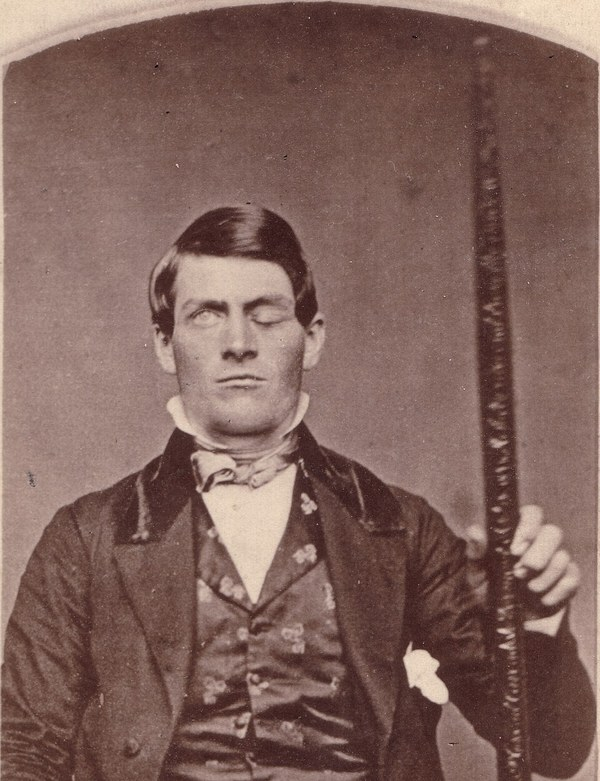
\includegraphics[height=5.0cm]{gage_portrait.jpg}\par
      {\scriptsize Գեյջը՝ իր ձողը ձեռքին}
    \end{column}
    \begin{column}{0.64\textwidth}
      \begin{itemize}
        \item Երկաթուղու շինարար, պատահական պայթյուն
        \item<2-> \textbf{Մոտ մեկ մետրանոց} երկաթյա ձողը մտավ ձախ աչքի տակից, անցավ ձախ \textbf{ճակատային բլթով} (frontal lobe) ու դուրս եկավ գանգի գագաթից
        \item<3-> Ձողն ընկավ մոտ \textbf{25 մետր} այն կողմ
      \end{itemize}
      \vspace{1mm}
      \onslide<4->{%
      \begin{bookquote}
        Մարդու գլուխը ձողին տյուլե վարագույրի չափ դիմադրություն ցույց տվեց։ Պարզաբանեմ. սա թղթով կտրվածք չէր։
      \end{bookquote}}
    \end{column}
  \end{columns}
\end{frame}

% He survived
\begin{frame}{Եվ նա ողջ մնաց}
  \begin{columns}[T]
    \begin{column}{0.5\textwidth}
      \begin{itemize}
        \item «Երկաթյա ձող գլխի միջով» այսօր էլ հարյուր տոկոսով մահացու է հնչում
        \item Իսկ սա 1800-ականներն էին, երբ ոտքի մատը խփելը կարող էր գանգրենայից մահ նշանակել
        \item<2-> Բայց Գեյջը ապրեց ևս \textbf{մոտ 12 տարի}
      \end{itemize}
      \vspace{1mm}
      \onslide<3->{%
      \begin{card}[colback=mint!35!cardwhite]
        \textbf{Ինչու}. ձողը հարթ ու սուր էր ու այնքան արագ, որ վերքը «մաքուր» ստացվեց։ Իսկ մյուս կիսագունդը ստանձնեց գործի մի մասը։
      \end{card}}
    \end{column}
    \begin{column}{0.44\textwidth}
      \onslide<4->{%
      \begin{scienceupdate}
        Գրքում՝ ձողը ոչնչացրեց ձախ ճակատային բլթի «գրեթե ամբողջը»։ 2012-ի վերակառուցումը ցույց տվեց. վնասվել էր կեղևի \textbf{մոտ 4\%}-ը, բայց սպիտակ նյութի (white matter) \textbf{10\%-ից ավելին}, այսինքն՝ մասերի միջև \textbf{կապերը}։
      \end{scienceupdate}}
    \end{column}
  \end{columns}
  \source{Van Horn et al., PLoS ONE, 2012}
\end{frame}

% The famous personality change
\begin{frame}{Նույն մարդը, թե՞ ուրիշ մարդ}
  \begin{columns}[T]
    \begin{column}{0.47\textwidth}
      \begin{card}[colback=mint!35!cardwhite]
        \centering\mascot[1.2cm]{happy}\par
        {\blackfont Մինչև վթարը}\par\smallskip
        \raggedright Մեղմ բնավորությամբ, աշխատասեր տղա
      \end{card}
    \end{column}
    \begin{column}{0.47\textwidth}
      \onslide<2->{%
      \begin{card}[colback=brainpink!30!cardwhite]
        \centering\mascot[1.2cm]{angry}\par
        {\blackfont Վթարից հետո (ըստ պատմությունների)}\par\smallskip
        \raggedright Անպատասխանատու, դյուրագրգիռ, հայհոյող, նույնիսկ «խելագար»
      \end{card}}
    \end{column}
  \end{columns}
  \vspace{1mm}
  \onslide<3->{%
  \begin{card}[colback=butter!45!cream]
    \centering Դուալիզմը լուրջ խնդրի առաջ կանգնեց. եթե ուղեղի վնասը փոխում է բնավորությունը, ուրեմն \textbf{անհատականությունն ուղեղի աշխատանքն է}։
  \end{card}}
\end{frame}

% Myth or fact: Gage never worked again
\begin{frame}{Առասպել, թե՞ փաստ \#1}
  \mythorfact{Վթարից հետո Գեյջը այլևս երբեք նորմալ չաշխատեց}{ԱՌԱՍՊԵԼ}{pinkdark}{%
    \begin{card}[colback=brainpink!25!cardwhite]
      Կյանքի վերջին տարիներին նա երկար ժամանակ \textbf{դիլիժանսի կառապան} էր. մեծ պատասխանատվությամբ ու մարդկանց հետ անընդհատ շփմամբ աշխատանք։ Եթե նույնիսկ բնավորությունը փոխվել էր, հետո նորից լավացել էր։
    \end{card}}
\end{frame}

% Why the extreme claims persist
\begin{frame}{Ինչու են պատմություններն այդքան սարսափելի}
  \begin{columns}[c]
    \begin{column}{0.56\textwidth}
      \begin{itemize}
        \item Այդ ժամանակի հոգեբանները (հարուստ, ինքնագոհ տղամարդիկ) Գեյջի դեպքով գովազդում էին \textbf{իրենց տեսությունները}
        \item<2-> Ամենածայրահեղ պնդումները հայտնվեցին \textbf{նրա մահից հետո}, երբ հերքող չկար։ Գեյջը Ֆեյսբուքից չէր իմանալու
        \item<3-> Ֆրենոլոգ Նելսոն Սայզերը գրեց, որ ձողը վնասել է «բարության» ու «ակնածանքի» «օրգանները». «դրա համար էլ հայհոյում է»
      \end{itemize}
    \end{column}
    \begin{column}{0.38\textwidth}
      \centering
      \onslide<3->{%
      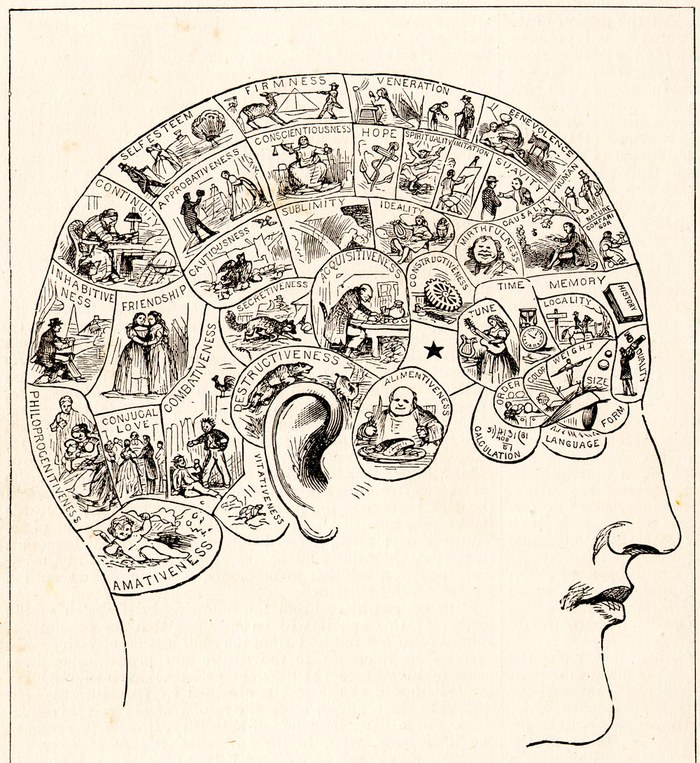
\includegraphics[height=4.8cm]{phrenology_chart.jpg}\par
      {\scriptsize Ֆրենոլոգիական քարտեզ, 19-րդ դար}}
    \end{column}
  \end{columns}
  \onslide<3->{\source{Macmillan, An Odd Kind of Fame, 2000}}
\end{frame}

% Two lasting lessons, and a definition
\begin{frame}{Գեյջի երկու դասը}
  \begin{columns}[T]
    \begin{column}{0.47\textwidth}
      \begin{card}[colback=mint!35!cardwhite]
        \emoji[1.4em]{brain}\ {\blackfont 1. Անհատականությունն ուղեղից է}\par\smallskip
        Վնասիր ուղեղը, ու մարդը կարող է փոխվել
      \end{card}
    \end{column}
    \begin{column}{0.47\textwidth}
      \onslide<2->{%
      \begin{card}[colback=peach!35!cardwhite]
        \emoji[1.4em]{ruler}\ {\blackfont 2. Այն չափելը տանջանք է}\par\smallskip
        IQ թեստերին դեռ կես դար կար։ Ինչպե՞ս չափել, թե ինչքան է Գեյջը փոխվել
      \end{card}}
    \end{column}
  \end{columns}
  \vspace{3mm}
  \onslide<3->{%
  \begin{card}[colback=lavender!35!cardwhite]
    {\blackfont\small Սահմանում, որի հետ համաձայն են հոգեբանների մեծ մասը} {\scriptsize (Phares \& Chaplin)}\par\smallskip
    Անհատականությունը մտքերի, զգացմունքների ու վարքի այն բնորոշ \textbf{նախշն} է, որը մի մարդուն \textbf{տարբերում է} մյուսից ու \textbf{պահպանվում է} ժամանակի ու իրավիճակների ընթացքում։
  \end{card}}
\end{frame}

% ===== Section 1: "Nothing personal", personality tests (~25 min) =====
\topicopener{masks}{Թեստեր}{Ոչինչ անձնական}{Անհատականության թեստերի կասկածելի օգտագործումը}{confused}

% Burnett and his sister
\begin{frame}{Բըրնեթն ու իր քույրը}
  \begin{columns}[T]
    \begin{column}{0.47\textwidth}
      \begin{card}[colback=lavender!35!cardwhite]
        \centering\mascot[1.1cm]{sleepy}\par
        {\blackfont Դինը}\par\smallskip
        \raggedright Այնքան հանգիստ, որ պետք էր հրել՝ համոզվելու, որ ուշքի է։ Այսօր՝ \textbf{նեյրոգիտնական} \emoji{brain}
      \end{card}
    \end{column}
    \begin{column}{0.47\textwidth}
      \onslide<2->{%
      \begin{card}[colback=peach!40!cardwhite]
        \centering\mascot[1.1cm]{panic}\par
        {\blackfont Քույրը՝ Քեյթին}\par\smallskip
        \raggedright Մեղմ ասած՝ գերակտիվ մղձավանջ։ Այսօր՝ \textbf{կեքսերի} (cupcake) վարպետ \emoji{cake}
      \end{card}}
    \end{column}
  \end{columns}
  \vspace{1mm}
  \onslide<3->{%
  \begin{card}[colback=butter!45!cream]
    Նույն ծնողները, նույն ժամանակը, նույն փոքրիկ գյուղը Ուելսի հովտում, շատ նման ԴՆԹ։ Եվ բոլորովին \textbf{տարբեր} անհատականություններ։
  \end{card}}
\end{frame}

% Fingerprints and a plastic fork
\begin{frame}{Մատնահետքեր ու պլաստիկ պատառաքաղ}
  \begin{columns}[c]
    \begin{column}{0.52\textwidth}
      \begin{itemize}
        \item Եթե նույն ընտանիքի երեխաները այսքան տարբեր են, ի՞նչ շանս ունենք կանխատեսել \textbf{երկու անծանոթի} անհատականությունը
        \item<2-> Մատնահետքը մաշկի վրա ընդամենը ակոսների նախշ է, բայց երկրի վրա գրեթե բոլորինը \textbf{յուրահատուկ} է
        \item<3-> Իսկ անհատականությունը տիեզերքի ամենաբարդ բանի՝ ուղեղի անհամար կապերի արդյունքն է
      \end{itemize}
    \end{column}
    \begin{column}{0.42\textwidth}
      \centering
      \onslide<4->{%
      \begin{bookquote}
        Գրավոր թեստով մարդու անհատականությունը որոշել փորձելը նույնն է, ինչ Ռաշմոր լեռան դեմքերը \textbf{պլաստիկ պատառաքաղով} քանդակելը։
      \end{bookquote}
      \bigemoji[1.2cm]{mountain}\ \raisebox{0.3cm}{\Large +}\ \bigemoji[1.2cm]{forkknife}}
    \end{column}
  \end{columns}
\end{frame}

% Few building blocks, endless variety
\begin{frame}{Բայց...}
  \centering
  % Few building blocks, endless variety: 3 fingerprint patterns, 4 DNA letters, 3 primary colours
% -> personality as a unique mix of a few traits (book: "Nothing personal"). Groups appear on clicks 1-3, the rule on 4.
\begin{tikzpicture}[lbl/.style={font=\small, text=plum, align=center},
    head/.style={font=\blackfont\normalsize, text=plum, align=center},
    ridge/.style={plum, line width=0.55pt}]
  % ---- fingerprints: arch, loop, whorl
  \begin{scope}[shift={(-4.7,0)}]
    \node[head] at (0,1.35) {Մատնահետքեր};
    % arch
    \begin{scope}[shift={(-1.15,0)}]
      \begin{scope}\clip (0,0) ellipse (0.45 and 0.6);
        \foreach \y in {-0.75,-0.62,...,0.6}{\draw[ridge] (-0.5,\y) .. controls (0,\y+0.4) .. (0.5,\y);}
      \end{scope}
      \draw[plum, line width=0.9pt] (0,0) ellipse (0.45 and 0.6);
      \node[lbl] at (0,-0.95) {կամար};
    \end{scope}
    % loop
    \begin{scope}
      \begin{scope}\clip (0,0) ellipse (0.45 and 0.6);
        \foreach \r in {0.07,0.17,0.27,0.37,0.47}{\draw[ridge] (0.6,\r-0.1) -- (0,\r-0.1) arc (90:270:\r) -- (0.6,-\r-0.1);}
        \foreach \y in {0.47,0.57,0.67}{\draw[ridge] (-0.6,\y) .. controls (0,\y+0.12) .. (0.6,\y);}
      \end{scope}
      \draw[plum, line width=0.9pt] (0,0) ellipse (0.45 and 0.6);
      \node[lbl] at (0,-0.95) {օղակ};
    \end{scope}
    % whorl
    \begin{scope}[shift={(1.15,0)}]
      \begin{scope}\clip (0,0) ellipse (0.45 and 0.6);
        \foreach \r in {0.06,0.15,...,0.65}{\draw[ridge] (0,0) ellipse [x radius=\r, y radius=1.3*\r];}
      \end{scope}
      \draw[plum, line width=0.9pt] (0,0) ellipse (0.45 and 0.6);
      \node[lbl] at (0,-0.95) {պտույտ};
    \end{scope}
    \node[lbl, font=\blackfont\small] at (0,-1.55) {3 տեսակ};
  \end{scope}
  % ---- DNA letters
  \begin{scope}[shift={(0,0)}, visible on=<2->]
    \node[head] at (0,1.35) {ԴՆԹ (DNA)};
    \foreach \x/\l/\c in {-1.2/G/mint, -0.4/A/peach, 0.4/T/lavender, 1.2/C/butter}{
      \node[circle, draw=plum, line width=0.8pt, fill=\c, minimum size=0.72cm, font=\blackfont\large, text=plum] at (\x,0.05) {\l};}
    \node[lbl] at (0,-0.95) {նուկլեոտիդներ};
    \node[lbl, font=\blackfont\small] at (0,-1.55) {4 «տառ»};
  \end{scope}
  % ---- primary colours
  \begin{scope}[shift={(4.7,0)}, visible on=<3->]
    \node[head] at (0,1.35) {Գույներ};
    \fill[amRed, fill opacity=0.65] (-0.3,0.2) circle (0.5);
    \fill[amBlue, fill opacity=0.65] (0.3,0.2) circle (0.5);
    \fill[amOrange, fill opacity=0.65] (0,-0.3) circle (0.5);
    \node[lbl] at (0,-0.95) {կարմիր, կապույտ, դեղին};
    \node[lbl, font=\blackfont\small] at (0,-1.55) {3 հիմնական};
  \end{scope}
  % ---- the rule
  \node[pbox=lavender, text width=10.5cm, font=\normalsize, visible on=<4->] at (0,-2.75)
    {Քիչ բաղադրիչ $\rightarrow$ անվերջ բազմազանություն։ Գուցե անհատականությունն էլ մի քանի \textbf{գծի} (traits) յուրահատուկ համադրություն է։};
\end{tikzpicture}

\end{frame}

% Traits
\begin{frame}{Գծերը (traits)}
  \begin{columns}[c]
    \begin{column}{0.47\textwidth}
      \begin{itemize}
        \item Այսօրվա տեսությունները. անհատականության մեջ կան կանխատեսելի, ճանաչելի բաղադրիչներ՝ \textbf{գծեր} (traits)
        \item<2-> Գծերը բոլորինն են նույնը, տարբեր է դրանց \textbf{համադրությունն} ու «չափաբաժինը»
        \item<3-> Ինչպես կարմիրից, կապույտից ու դեղինից ստացվում է գրեթե ցանկացած գույն
      \end{itemize}
    \end{column}
    \begin{column}{0.49\textwidth}
      \onslide<4->{%
      \begin{bookquote}
        «Ուրեմն մարդու անհատականությունը \textbf{իր} գծերի յուրահատուկ նախշն է» (Ջ. Պ. Գիլֆորդ, 1959)։\par\smallskip
        Բնօրինակում «իր»-ը \textbf{his} է՝ տղամարդունը։ 1950-ականներն էին. կանայք անհատականություն ունենալու իրավունք ստացան միայն 1970-ականների կեսերին։
      \end{bookquote}}
    \end{column}
  \end{columns}
\end{frame}

% The Big Five
\begin{frame}{«Մեծ հնգյակը» (Big Five)}
  \centering
  {\small Ամեն գծում յուրաքանչյուրս երկու ծայրահեղության միջև ենք}\par\smallskip
  % The Big Five as five scales between two extremes (book: "Nothing personal"). Rows appear on clicks 1-5.
% Each row: letter, Armenian + English name, a bar with the low extreme under its left end and the high one under its right end.
\begin{tikzpicture}[
    letter/.style={circle, draw=plum, line width=0.8pt, minimum size=0.72cm, font=\blackfont\large, text=plum, inner sep=0},
    tname/.style={anchor=west, font=\blackfont\small, text=plum, align=left},
    lowlbl/.style={anchor=north west, font=\footnotesize, text=plum, inner sep=1pt},
    highlbl/.style={anchor=north east, font=\footnotesize, text=plum, inner sep=1pt},
  ]
  \foreach \i/\L/\c/\name/\eng/\lo/\hi in {
      1/O/mint/Բացություն/Openness/{սովորական, ծանոթ}/{նոր փորձառություններ},
      2/C/butter/Բարեխղճություն/Conscientiousness/{ինքնաբուխ, անկազմակերպ}/{պլան, կարգ},
      3/E/peach/Էքստրավերսիա/Extraversion/{ինտրովերտ, հանգիստ}/{էքստրավերտ, շփվող},
      4/A/lavender/Բարեհամբույրություն/Agreeableness/{նախ՝ իր ուզածը}/{ներդաշնակություն},
      5/N/brainpink/Նևրոտիզմ/Neuroticism/{հանգիստ, կայուն}/{անհանգիստ, լարված}}{
    \begin{scope}[yshift={-(\i-3)*1.0cm}, visible on=<\i->]
      \node[letter, fill=\c] at (-6.9,0) {\L};
      \node[tname] at (-6.4,0) {\name\\ {\mediumfont\scriptsize \eng}};
      \shade[left color=\c!20!cardwhite, right color=\c, rounded corners=1.5mm] (-2.3,0.06) rectangle (5.4,0.34);
      \draw[plum, line width=0.7pt, rounded corners=1.5mm] (-2.3,0.06) rectangle (5.4,0.34);
      \node[lowlbl] at (-2.3,0.0) {\lo};
      \node[highlbl] at (5.4,0.0) {\hi};
    \end{scope}}
\end{tikzpicture}

\end{frame}

% The rotten-pork exhibition, part 1
\begin{frame}{Նեխած մսից քանդակներ. հրավեր}
  \begin{traitbox}{mint}{\emoji[1em]{palette}\ O. Բացություն}
    \begin{minipage}[t]{0.48\linewidth}\raggedright
      {\blackfont Բարձր.} «Իհա՛րկե։ Նեխած մսից արվեստ երբեք չեմ տեսել, հրաշալի է լինելու»։
    \end{minipage}\hfill
    \begin{minipage}[t]{0.48\linewidth}\raggedright
      {\blackfont Ցածր.} «Ոչ։ Դա քաղաքի ուրիշ ծայրում է, ուրեմն դուր չի գա»։
    \end{minipage}
  \end{traitbox}
  \onslide<2->{%
  \begin{traitbox}{butter}{\emoji[1em]{clipboard}\ C. Բարեխղճություն}
    \begin{minipage}[t]{0.48\linewidth}\raggedright
      {\blackfont Բարձր.} Կգա, բայց նախ կգտնի լավագույն ավտոբուսը ու կպատվաստվի տետանուսի դեմ։
    \end{minipage}\hfill
    \begin{minipage}[t]{0.48\linewidth}\raggedright
      {\blackfont Ցածր.} «Տասը րոպեից այնտեղ եմ»։ Ղեկավարին չի էլ հարցնի, իսկ ցուցահանդեսը կգտնի \textbf{հոտով}։
    \end{minipage}
  \end{traitbox}}
\end{frame}

% The rotten-pork exhibition, part 2
\begin{frame}{Նույն հրավերը, մյուս գծերը}
  \begin{traitbox}{peach}{\emoji[1em]{camera}\ E. Էքստրավերսիա}
    \begin{minipage}[t]{0.48\linewidth}\raggedright
      {\blackfont Էքստրավերտ.} Կգա իր շտապ սարքած քանդակով ու կնկարվի բոլոր նմուշների կողքին՝ Instagram-ի համար։
    \end{minipage}\hfill
    \begin{minipage}[t]{0.48\linewidth}\raggedright
      {\blackfont Ինտրովերտ.} Ոչ մեկի հետ այնքան երկար չի խոսի, որ հրավեր ստանա։
    \end{minipage}
  \end{traitbox}
  \vspace{1mm}
  \onslide<2->{%
  \begin{traitbox}{lavender}{\emoji[1em]{handshake}\ A. Բարեհամբույրություն}
    \begin{minipage}[t]{0.48\linewidth}\raggedright
      {\blackfont Բարձր.} Իհարկե կգա, բայց միայն եթե հրավիրողը դեմ չէ. չի ուզում նեղություն տալ։
    \end{minipage}\hfill
    \begin{minipage}[t]{0.48\linewidth}\raggedright
      {\blackfont Ցածր.} Նրան ընդհանրապես ոչ ոք ոչ մի տեղ չի հրավիրի։
    \end{minipage}
  \end{traitbox}}
\end{frame}

% The rotten-pork exhibition, part 3 + chat
\begin{frame}{Եվ վերջինը}
  \begin{columns}[c]
    \begin{column}{0.56\textwidth}
      \begin{traitbox}{brainpink}{\emoji[1em]{fearful}\ N. Նևրոտիզմ}
        Նևրոտիկ մարդը հրավերը կմերժի ու \textbf{հիասքանչ մանրամասներով} կբացատրի՝ ինչու։\par\smallskip
        Տե՛ս՝ Վուդի Ալեն։
      \end{traitbox}
      \vspace{1mm}
      \onslide<2->{%
      \begin{chatbox}
        Իսկ դու ինչպե՞ս կպատասխանեիր այս հրավերին։ Գրիր մեկ նախադասություն։
      \end{chatbox}}
    \end{column}
    \begin{column}{0.38\textwidth}
      \centering
      \mascot[2.6cm]{scared}\par
      {\small\color{plum!70!cream}«...իսկ եթե այնտեղ հոտը...»}
    \end{column}
  \end{columns}
\end{frame}

% Consistency and Eysenck's arousal idea
\begin{frame}{Ինչու են ինտրովերտները խուսափում աղմուկից}
  \begin{columns}[c]
    \begin{column}{0.54\textwidth}
      \begin{itemize}
        \item Մեծ հնգյակի գծերը \textbf{կայուն} են. բարեհամբույրը բարեհամբույր է ամենուր
        \item<2-> Հանս Այզենկ. ինտրովերտների կեղևն առանց այն էլ ավելի «գրգռված» է (cortical arousal)
        \item<3-> Նրանց շատ գրգիռ պետք չէ, իսկ էքստրավերտները գրգիռ են \textbf{փնտրում}
      \end{itemize}
    \end{column}
    \begin{column}{0.42\textwidth}
      \centering
      \scalebox{0.78}{% Eysenck's idea: introverts start with higher cortical arousal, extroverts lower, so extroverts seek
% extra stimulation to reach a comfortable level. Schematic, not data. The extrovert's top-up shows on click 3.
\begin{tikzpicture}[lbl/.style={font=\small, text=plum, align=center}]
  % comfort line
  \draw[plum!70, dashed, line width=0.9pt] (-2.1,2.9) -- (2.3,2.9);
  \node[anchor=east, font=\footnotesize, text=plum, align=right] at (-2.15,2.9) {հարմարավետ\\ մակարդակ};
  % introvert tube
  \fill[lavender, rounded corners=2mm] (-1.9,0) rectangle (-0.9,2.65);
  \draw[plum, line width=0.9pt, rounded corners=2mm] (-1.9,0) rectangle (-0.9,3.6);
  \node[lbl, font=\blackfont\small] at (-1.4,-0.35) {Ինտրովերտ};
  \node[lbl, font=\footnotesize] at (-1.4,-0.85) {արդեն գրեթե\\ բավական է};
  % extrovert tube
  \fill[peach, rounded corners=2mm] (0.9,0) rectangle (1.9,1.2);
  \fill[amOrange!70, visible on=<3->] (0.9,1.2) rectangle (1.9,2.9);
  \draw[plum, line width=0.9pt, rounded corners=2mm] (0.9,0) rectangle (1.9,3.6);
  \node[lbl, font=\blackfont\small] at (1.4,-0.35) {Էքստրավերտ};
  \node[lbl, font=\footnotesize] at (1.4,-0.85) {պետք է\\ լրացնել};
  \node[visible on=<3->] at (2.7,2.0) {\bigemoji[0.75cm]{party}};
  \node[visible on=<3->] at (2.7,1.1) {\bigemoji[0.75cm]{microphone}};
\end{tikzpicture}
}
    \end{column}
  \end{columns}
\end{frame}

% Brain scans
\begin{frame}{Գծերը ուղեղի սկաներում}
  \begin{columns}[T]
    \begin{column}{0.47\textwidth}
      \begin{card}[colback=brainpink!30!cardwhite]
        \emoji[1.3em]{fearful}\ {\blackfont Նևրոտիզմ} {\scriptsize (Taki et al.)}\par\smallskip
        \textbf{Ավելի փոքր}՝ նախաճակատային կեղևի մի մասը ու ձախ հիպոկամպի հետին մասը, \textbf{ավելի մեծ}՝ միջին գոտկային գալարը (mid-cingulate)\par
        \onslide<2->{\smallskip Գուցե նևրոտիկ մարդը դժվար է սովորում, որ իր տագնապները \textbf{չեն արդարանում}։}
      \end{card}
    \end{column}
    \begin{column}{0.47\textwidth}
      \onslide<3->{%
      \begin{card}[colback=peach!40!cardwhite]
        \emoji[1.3em]{party}\ {\blackfont Էքստրավերսիա}\par\smallskip
        Ավելի ակտիվ է \textbf{ակնակապային ճակատային կեղևը} (orbitofrontal cortex), որ կապված է որոշումների հետ։\par\smallskip
        Գուցե դրա համար են էքստրավերտներն ավելի հաճախ գործում։ Բըրնեթն ինքն էլ հարցական է դնում։
      \end{card}}
    \end{column}
  \end{columns}
\end{frame}

% Genes
\begin{frame}{Անհատականությունն ու գեները}
  \begin{columns}[c]
    \begin{column}{0.56\textwidth}
      \centering
      % Heritability of the Big Five, Jang, Livesley & Vernon, J. Personality 1996 (the book's source):
% 123 identical + 127 fraternal twin pairs; broad genetic influence O 61, C 44, E 53, A 41, N 41 %.
% The book gives the range "40 to 60 per cent" (butter band). ytick listed explicitly (see _learnings pgfplots note).
\begin{tikzpicture}
  \begin{axis}[
      set layers,
      width=5.4cm, height=5.0cm,
      xbar, bar width=0.42cm,
      xmin=0, xmax=80,
      symbolic y coords={N, A, E, C, O},
      ytick={N, A, E, C, O},
      yticklabels={Նևրոտիզմ, Բարեհամբույրություն, Էքստրավերսիա, Բարեխղճություն, Բացություն},
      xtick={0,20,40,60}, xticklabel={\pgfmathprintnumber{\tick}\%},
      tick label style={font=\footnotesize, text=plum}, axis line style={plum},
      axis x line*=bottom, axis y line*=left, xmajorgrids, grid style={plum!10},
      nodes near coords={\pgfmathprintnumber{\pgfplotspointmeta}\%},
      nodes near coords style={font=\blackfont\footnotesize, text=plum},
      enlarge y limits=0.13,
    ]
    \begin{pgfonlayer}{axis background}
      \fill[butter!80] ({axis cs:40,N}|-{rel axis cs:0,0}) rectangle ({axis cs:60,O}|-{rel axis cs:0,1});
    \end{pgfonlayer}
    \addplot[fill=amBlue, draw=none] coordinates {(41,N) (41,A) (53,E) (44,C) (61,O)};
  \end{axis}
\end{tikzpicture}
\par
      {\scriptsize Գեների ազդեցությունը (heritability). դեղին շերտը՝ գրքի «40-60\%»-ը}
    \end{column}
    \begin{column}{0.4\textwidth}
      \begin{itemize}
        \item Երկվորյակներ. միաձվայիններն ունեն նույն գեները, երկձվայինները՝ մոտ կեսը։ Եթե առաջինները իրար ավելի նման են, գեներն են ազդում
        \item<2-> Գրքում՝ «գրեթե 300 զույգ», իրականում \textbf{250} էր
        \item<3-> Նույն ընտանիքում մեծանալը գրեթե \textbf{ոչինչ} չէր բացատրում։ Բարև, Քեյթի \emoji{cake}
      \end{itemize}
    \end{column}
  \end{columns}
  \source{Jang, Livesley \& Vernon, J. Personality, 1996}
\end{frame}

% So what's the issue?
\begin{frame}
  \bigquestion{Հինգ գիծ, ուղեղի մասեր ու գեներ։ Ո՞րն է խնդիրը}{Երեք լուրջ առարկություն}
\end{frame}

% Critique 1: incomplete, outward only
\begin{frame}{Առարկություն 1. ոչ ամբողջական}
  \begin{columns}[c]
    \begin{column}{0.46\textwidth}
      \begin{itemize}
        \item Լավ ընդհանուր շրջանակ է, բայց որտե՞ղ է \textbf{հումորը}։ Իսկ կրոնականությունը, սնահավատությունը, բռնկուն բնավորությո՞ւնը
        \item<2-> Քննադատները. այն նկարագրում է «արտաքին» անհատականությունը, այն, ինչ \textbf{ուրիշները տեսնում են}
        \item<2-> Իսկ մեծ մասը կատարվում է գլխիդ ներսում ու միշտ չէ, որ երևում է վարքում
      \end{itemize}
    \end{column}
    \begin{column}{0.5\textwidth}
      \centering
      \scalebox{0.9}{% Critique of the Big Five (book): it describes the "outward" personality others can see;
% much of personality (humour, beliefs, prejudices) stays inside the head. The hidden part shows on click 2.
\begin{tikzpicture}[lbl/.style={font=\small, text=plum, align=center}]
  % water
  \fill[mint!45] (-3.4,0) rectangle (3.4,-3.3);
  \draw[plum, line width=0.9pt, decorate, decoration={snake, amplitude=0.6mm, segment length=5mm}] (-3.4,0) -- (3.4,0);
  % visible tip
  \filldraw[fill=cardwhite, draw=plum, line width=0.9pt]
    (-1.3,0) -- (-0.6,1.5) -- (-0.1,1.1) -- (0.5,1.9) -- (1.4,0) -- cycle;
  \node[lbl, font=\blackfont\small] at (0.05,0.45) {Մեծ հնգյակ};
  \node[lbl, font=\footnotesize, anchor=west] at (1.6,1.15) {ինչ որ ուրիշները\\ տեսնում են};
  % hidden part
  \begin{scope}[visible on=<2->]
    \filldraw[fill=lavender!55, draw=plum, line width=0.9pt, dashed]
      (-1.3,0) -- (-2.7,-1.2) -- (-1.9,-2.9) -- (1.1,-3.1) -- (2.8,-1.6) -- (1.4,0) -- cycle;
    \node[lbl, text width=4.4cm, font=\footnotesize] at (0.05,-1.5) {\emoji{laughing}\ հումոր \quad \emoji{crystalball}\ սնահավատություն\\[1mm] \emoji{thought}\ համոզմունքներ \quad \emoji{bomb}\ բռնկվածություն\\[1mm] \emoji{lock}\ նախապաշարմունքներ};
  \end{scope}
\end{tikzpicture}
}
    \end{column}
  \end{columns}
\end{frame}

% Critique 2: cause or consequence
\begin{frame}{Առարկություն 2. պատճա՞ռ, թե՞ հետևանք}
  \begin{columns}[c]
    \begin{column}{0.5\textwidth}
      \centering
      \begin{tikzpicture}
        \node[pbox=lavender, text width=3.5cm, minimum height=1.3cm] (p) at (0,0) {\emoji{masks}\\ \textbf{Անհատականություն}};
        \node[pbox=mint, text width=3.5cm, minimum height=1.3cm] (b) at (0,-3) {\emoji{brain}\\ \textbf{Ուղեղի կառուցվածք}};
        \draw[arr] ([xshift=-6mm]b.north) -- node[left, font=\scriptsize, text=plum, align=right] {այսպես ենք\\ կարծում} ([xshift=-6mm]p.south);
        \draw[arr, amOrange!90!black, visible on=<2->] ([xshift=6mm]p.south) -- node[right, font=\scriptsize, text=plum, align=left] {իսկ գուցե\\ այսպե՞ս} ([xshift=6mm]b.north);
      \end{tikzpicture}
    \end{column}
    \begin{column}{0.46\textwidth}
      \begin{itemize}
        \item Ուղեղը ճկուն է ու \textbf{փոխվում է} իր փորձառությանը համապատասխան
        \item<2-> Շատ նևրոտիկ կամ էքստրավերտ մարդը ապրում է ուրիշ փորձառություններ, ու ուղեղը կարող է \textbf{դրանք} արտացոլել
        \item<3-> Ու սա այն դեպքում, եթե տվյալները 100\%-ով հաստատված են։ Իսկ դրանք հաստատված չեն
      \end{itemize}
    \end{column}
  \end{columns}
\end{frame}

% Critique 3: factor analysis = buckets of rain
\begin{frame}{Առարկություն 3. անձրևի դույլեր}
  \begin{columns}[c]
    \begin{column}{0.44\textwidth}
      \begin{itemize}
        \item Մեծ հնգյակը ծնվել է \textbf{գործոնային վերլուծությունից} (factor analysis, 4-րդ գլուխ). տարբեր մարդիկ նորից ու նորից գտել են այս հինգը
        \item<2-> Բայց վերլուծությունը միայն նկարագրում է եղած տվյալները
        \item<2-> Դույլերով կիմանաս, թե որտեղ է շատ անձրև գալիս։ Դա \textbf{սկիզբն է}, ոչ թե պատասխանը
      \end{itemize}
    \end{column}
    \begin{column}{0.52\textwidth}
      \centering
      \scalebox{0.9}{% Burnett's analogy for factor analysis: buckets across town show WHERE most rain falls, not WHY it rains.
% The "why?" cloud shows on click 2.
\begin{tikzpicture}[lbl/.style={font=\small, text=plum, align=center}]
  \foreach \x/\lev/\drops/\name in {-3.3/0.25/3/Ա, -1.1/0.95/8/Բ, 1.1/0.5/5/Գ, 3.3/0.3/3/Դ}{
    \node at (\x,3.05) {\bigemoji[0.8cm]{raincloud}};
    \foreach \k in {1,...,\drops}{
      \pgfmathsetmacro{\dx}{-0.42+0.84*(\k-0.5)/\drops}
      \draw[amBlue!70, line width=0.9pt] ({\x+\dx},{2.45-0.08*mod(\k,2)}) -- ++(-0.06,-0.3);
      \draw[amBlue!70, line width=0.9pt] ({\x+\dx+0.05},{1.75-0.1*mod(\k,3)}) -- ++(-0.06,-0.3);}
    \begin{scope}
      \clip (\x-0.42,0) -- (\x+0.42,0) -- (\x+0.55,1.15) -- (\x-0.55,1.15) -- cycle;
      \fill[amBlue!45] (\x-0.6,0) rectangle (\x+0.6,\lev);
    \end{scope}
    \draw[plum, line width=0.9pt, line join=round] (\x-0.55,1.15) -- (\x-0.42,0) -- (\x+0.42,0) -- (\x+0.55,1.15);
    \draw[plum, line width=0.7pt] (\x-0.5,1.15) arc (180:0:0.5 and 0.35);
    \node[lbl, font=\blackfont\small] at (\x,-0.35) {\name};
  }
  \node at (-0.25,0.4) {\bigemoji[0.45cm]{trophy}};
  \node[pbox=lavender, text width=4.8cm, visible on=<2->] at (0,-1.35)
    {\emoji{question}\ \textbf{Ինչու} է անձրև գալիս\\ ու ինչպես են ամպերը գոյանում};
\end{tikzpicture}
}
    \end{column}
  \end{columns}
\end{frame}

% Type A and Type B
\begin{frame}{«Ա» և «Բ» տիպեր}
  \begin{columns}[T]
    \begin{column}{0.47\textwidth}
      \begin{card}[colback=brainpink!30!cardwhite]
        \emoji[1.4em]{rage}\ {\blackfont Ա տիպ} {\scriptsize (Type A)}. մրցակցող, հաջողության ձգտող, անհամբեր, ագրեսիվ։ Հաճախ դառնում են ղեկավար
      \end{card}
    \end{column}
    \begin{column}{0.47\textwidth}
      \begin{card}[colback=mint!35!cardwhite]
        \emoji[1.4em]{couch}\ {\blackfont Բ տիպ} {\scriptsize (Type B)}. այս ամենը չեն\par\smallskip
        {\scriptsize Ֆրիդման ու Ռոզենման, 1950-ականներ (գրքում՝ «Ռոզենհան»)}
      \end{card}
    \end{column}
  \end{columns}
  \begin{itemize}
    \item<2-> Ա տիպի մարդիկ \textbf{երկու անգամ ավելի հաճախ} էին ինֆարկտ ստանում։ Անհատականությունը բառացիորեն կարող է սպանել \emoji{anatomicalheart}
    \item<3-> Հետագա հետազոտություններ. մեղավորը գուցե ծխելն էր, վատ սնունդը ու ամեն ութ րոպեն մեկ ենթակաների վրա գոռալը
    \item<4-> Երկու տիպը չափազանց ընդհանուր էր, ու ուշադրությունն անցավ ավելի մանրամասն \textbf{գծերին}
  \end{itemize}
\end{frame}

% Lexical hypothesis
\begin{frame}{Գծերը թաքնված են բառերի մեջ}
  \begin{columns}[c]
    \begin{column}{0.54\textwidth}
      \begin{itemize}
        \item Ֆրենսիս Գալթոնը (1800-ականներ) ու Ռեյմոնդ Քեթելը (1950-ականներ) լեզվում փնտրում էին մարդուն նկարագրող բառեր
        \item<2-> \textbf{Բառային վարկած} (lexical hypothesis). կարևոր տարբերությունների համար լեզուն բառ կունենա
        \item<3-> Բառերը հավաքեցին, խմբավորեցին, ու դրանցից «դուրս եկան» գծերը
      \end{itemize}
    \end{column}
    \begin{column}{0.4\textwidth}
      \onslide<2->{%
      \begin{card}[colback=brainpink!25!cardwhite]
        նյարդային, տագնապող, պարանոյիկ $\rightarrow$ \textbf{նևրոտիզմ}
      \end{card}
      \begin{card}[colback=lavender!35!cardwhite]
        շփվող, ընկերասեր $\rightarrow$ \textbf{բարեհամբույրություն}
      \end{card}}
      \onslide<4->{%
      \begin{chatbox}
        Գրիր \textbf{մեկ բառ}, որով կնկարագրեիր մարդու բնավորություն
      \end{chatbox}}
    \end{column}
  \end{columns}
\end{frame}

% Language and situations
\begin{frame}{Լեզուն ու իրավիճակը}
  \begin{columns}[T]
    \begin{column}{0.47\textwidth}
      \begin{card}[colback=peach!35!cardwhite]
        \emoji[1.4em]{speakinghead}\ {\blackfont Լեզուն}\par\smallskip
        Բառային մոտեցումը կախված է լեզվից, իսկ լեզուն տարբեր է տարբեր մշակույթներում ու անընդհատ փոխվում է
      \end{card}
    \end{column}
    \begin{column}{0.47\textwidth}
      \onslide<2->{%
      \begin{card}[colback=mint!35!cardwhite]
        \emoji[1.4em]{candle}\ {\blackfont Իրավիճակը}\par\smallskip
        Ոչ ոք ամեն տեղ նույն կերպ չի վարվում։ Էքստրավերտը թաղման կամ կարևոր գործնական հանդիպման ժամանակ էքստրավերտի պես չի պահի իրեն (եթե խորքային խնդիրներ չունի)
      \end{card}}
    \end{column}
  \end{columns}
  \vspace{1mm}
  \onslide<3->{%
  \begin{card}[colback=butter!45!cream]
    \centering Այս տեսակետը կոչվում է \textbf{սիտուացիոնիզմ} (situationism). վարքը որոշում է ոչ միայն անհատականությունը, այլև \textbf{իրավիճակը}։
  \end{card}}
\end{frame}

% Tests are fun
\begin{frame}{Բայց թեստերը զվարճալի են}
  \begin{columns}[c]
    \begin{column}{0.48\textwidth}
      \begin{itemize}
        \item Արագ հարցաշար, ու քեզ ասում են, թե որ «տիպին» ես պատկանում
        \item<2-> Մենք արդեն կարծիք ունենք մեր մասին, ու թեստը, որ \textbf{հաստատում է} այն, հաճելի է
        \item<3-> Թեկուզ թեստը մի վատ սարքված կայքում է, որ ամեն վեց վայրկյանը մեկ առաջարկում է գրանցվել օնլայն կազինոյում։ Թեստը թեստ է
      \end{itemize}
    \end{column}
    \begin{column}{0.46\textwidth}
      \onslide<3->{%
      \begin{popup}{գովազդ.exe}
        \centering\bigemoji[1cm]{slotmachine}\par\smallskip
        {\blackfont Դու ԷՔՍՏՐԱՎԵՐՏ ես։}\par
        Էքստրավերտները \textbf{հաղթում են}։ Գրանցվի՛ր կազինոյում հիմա
      \end{popup}}
    \end{column}
  \end{columns}
\end{frame}

% Rorschach
\begin{frame}{Ի՞նչ ես տեսնում}
  \begin{columns}[c]
    \begin{column}{0.5\textwidth}
      \centering
      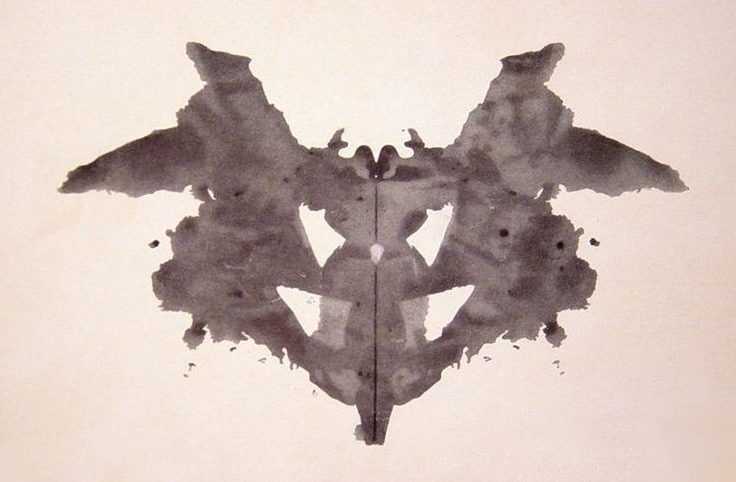
\includegraphics[width=\linewidth]{rorschach_card1.jpg}\par
      {\scriptsize Ռորշախի թեստի առաջին քարտը, 1921}
    \end{column}
    \begin{column}{0.46\textwidth}
      \begin{chatbox}
        Ի՞նչ ես տեսնում այս բծի մեջ։ Գրիր առաջին բանը, որ մտքովդ անցավ
      \end{chatbox}
      \vspace{1mm}
      \alt<3->{%
      \begin{card}[colback=brainpink!25!cardwhite]
        Հազար նման մարդ՝ հազար տարբեր պատասխան։ Լավ ցույց է տալիս անհատականության բարդությունը, բայց \textbf{ստուգել} հնարավոր չէ։
      \end{card}}{%
      \onslide<2->{%
      \begin{card}
        {\blackfont\small Բըրնեթի օրինակները}\par\smallskip
        «Կոկոնից դուրս եկող թիթեռներ»։ Կամ՝ «թերապևտիս պայթած գլուխը, որ չափից շատ հարցեր էր տալիս»։
      \end{card}}}
    \end{column}
  \end{columns}
\end{frame}

% Myth or fact: MBTI
\begin{frame}{Առասպել, թե՞ փաստ \#2}
  \mythorfact{4 տառով MBTI թեստը գիտականորեն հաստատված է}{ԱՌԱՍՊԵԼ}{pinkdark}{%
    \begin{card}[colback=brainpink!25!cardwhite]
      Աշխարհի ամենապոպուլյար թեստերից է ու միլիոնավոր դոլարներ արժե, բայց գիտական հանրությունը այն \textbf{չի ճանաչում}։ Ամենատխուր կիրառությունը՝ ընկերություններում։
    \end{card}}
\end{frame}

% MBTI
\begin{frame}{Մայերս-Բրիգս (MBTI)}
  \begin{columns}[c]
    \begin{column}{0.56\textwidth}
      \begin{itemize}
        \item Myers-Briggs Type \textbf{Indicator} (գրքում՝ Inventory)
        \item Լուրջ տեսք ունի. սանդղակներ, ամենահայտնին՝ էքստրավերտ-ինտրովերտ
        \item<2-> Բայց հիմնված է հին, \textbf{չստուգված ենթադրությունների} վրա, որոնք հավաքել են ոգևորված սիրողներ՝ \textbf{մեկ աղբյուրից}
        \item<3-> Բիզնեսը կառչեց դրանից, ու այսօր այն հարյուր հազարավոր ջատագովներ ունի
      \end{itemize}
    \end{column}
    \begin{column}{0.38\textwidth}
      \centering
      \onslide<4->{%
      \bigemoji[1.6cm]{crystalball}\par\medskip
      \begin{bookquote}
        Բայց հորոսկոպներն էլ ունեն։
      \end{bookquote}}
    \end{column}
  \end{columns}
\end{frame}

% Waiting skeleton + retest
\begin{frame}{Եվ դեռ սպասում ենք}
  \begin{columns}[c]
    \begin{column}{0.4\textwidth}
      \centering
      \begin{meme}[4.4cm]{waiting_skeleton.jpg}
        \memecap[text width=3.6cm]{0.5}{0.9}{MBTI-ի գիտական ապացույցները}
      \end{meme}
    \end{column}
    \begin{column}{0.54\textwidth}
      \onslide<2->{%
      \begin{scienceupdate}
        Լավ թեստը նույն մարդուն երկրորդ անգամ նույն արդյունքը պիտի տա։ MBTI-ն կրկին լրացնողների \textbf{մոտ կեսը} ընդամենը \textbf{5 շաբաթ անց} ստանում է \textbf{ուրիշ} տիպ։ Մեծ հնգյակի թեստերն այս առումով շատ ավելի կայուն են։
      \end{scienceupdate}}
    \end{column}
  \end{columns}
  \onslide<2->{\source{Pittenger, 1993, 2005}}
\end{frame}

% Why companies love it
\begin{frame}{Ինչու է այն սիրում բիզնեսը}
  \begin{columns}[c]
    \begin{column}{0.5\textwidth}
      \begin{itemize}
        \item Պարզ է ու հասկանալի
        \item Աշխատակիցներին բաժանում է հարմար \textbf{խմբերի}, որոնք իբր կանխատեսում են վարքը
        \item<3-> Գոնե տեսականորեն։ Գործնականում չի կարող աշխատել, որովհետև մարդիկ \textbf{բոլորովին էլ այդքան պարզ չեն}
      \end{itemize}
    \end{column}
    \begin{column}{0.46\textwidth}
      \centering
      \begin{tikzpicture}
        \node[pbox=lavender, text width=4.6cm] (i) at (0,1.1) {\emoji{door}\ \textbf{Ինտրովե՞րտ}\\ Թող մենակ աշխատի, մի խանգարեք};
        \node[pbox=peach, text width=4.6cm, visible on=<2->] (e) at (0,-0.9) {\emoji{megaphone}\ \textbf{Էքստրավե՞րտ}\\ Թող զբաղվի գովազդով ու շփումներով. նրանք դա սիրում են};
        \node[visible on=<3->] at (-1.6,-2.55) {\mascot[1.3cm]{confused}};
      \end{tikzpicture}
    \end{column}
  \end{columns}
\end{frame}

% The job application test
\begin{frame}{Աշխատանքի դիմումի թեստ}
  \begin{columns}[c]
    \begin{column}{0.5\textwidth}
      \begin{popup}{դիմում.exe}
        {\blackfont Հարց 7. Սիրու՞մ եք ուրիշների հետ աշխատել}\par\medskip
        $\square$\ Այո, թիմային աշխատանքը իմ ուժն է\par\smallskip
        $\square$\ Կախված է նախագծից\par\smallskip
        \onslide<2->{$\square$\ Ոչ։ Ուրիշները միջատներ են, որոնք կան միայն ճզմվելու համար}
      \end{popup}
    \end{column}
    \begin{column}{0.44\textwidth}
      \onslide<3->{%
      \begin{itemize}
        \item Թեստն աշխատում է, եթե դիմողը 100\% անկեղծ է ու գրեթե նույնքան միամիտ
        \item Շատերը «ապահով» են պատասխանում, ու արդյունքը \textbf{անիմաստ} է դառնում
      \end{itemize}}
      \onslide<4->{%
      \begin{poll}
        Ձեռք բարձրացրու, եթե թեստին երբևէ պատասխանել ես այնպես, ինչպես \textbf{«պետք է»}
      \end{poll}}
    \end{column}
  \end{columns}
\end{frame}

% Section end
\begin{frame}{Թեստերը՝ մեկ էջում}
  \begin{columns}[T]
    \begin{column}{0.47\textwidth}
      \begin{card}[colback=mint!35!cardwhite]
        \emoji[1.3em]{check}\ {\blackfont Մեծ հնգյակ}\par\smallskip
        Լավագույնն է, ինչ ունենք. կայուն գծեր, կապ ուղեղի ու գեների հետ։ Բայց ոչ ամբողջական, ու չգիտենք՝ որն է պատճառը, որը՝ հետևանքը
      \end{card}
    \end{column}
    \begin{column}{0.47\textwidth}
      \begin{card}[colback=brainpink!25!cardwhite]
        \emoji[1.3em]{cross}\ {\blackfont MBTI ու օնլայն թեստեր}\par\smallskip
        Զվարճալի են, բայց գիտական չեն։ Ու մի որոշիր աշխատակցի ճակատագիրը չորս տառով
      \end{card}
    \end{column}
  \end{columns}
  \vspace{3mm}
  \onslide<2->{%
  \begin{bookquote}
    Անհատականության թեստերն ավելի օգտակար կլինեին, եթե մեր անհատականությունները չխանգարեին։
  \end{bookquote}}
\end{frame}

% ---------------------------------------------------------------- break
\begin{frame}[plain]
  \begin{tikzpicture}[remember picture, overlay]
    \fill[butter!60!cream] (current page.south west) rectangle (current page.north east);
    \node at ([yshift=8mm]current page.center) {\mascot[4cm]{sleepy}};
    \node[anchor=north, font=\titlefont\fontsize{30}{32}\selectfont, text=plum] at ([yshift=-17mm]current page.center) {Ընդմիջում};
    \node[anchor=north, font=\mediumfont\large, text=plum] at ([yshift=-31mm]current page.center)
      {5 րոպե \emoji{coffee}\quad Կանգնիր, ձգվիր, ջուր խմիր};
  \end{tikzpicture}
\end{frame}

% ===== Section 2: "Do blow your fuse", anger (~18 min) =====
\topicopener{angry}{Զայրույթ}{Պայթի՛ր, կարելի է}{Ինչպես է աշխատում զայրույթը, ու ինչու է այն երբեմն օգտակար}{angry}

% Hulk
\begin{frame}{«Ինձ չես հավանի, երբ բարկացած եմ»}
  \begin{columns}[c]
    \begin{column}{0.42\textwidth}
      \centering
      \mascot[2.2cm]{angry}\par\medskip
      \begin{card}[colback=mint!40!cardwhite]
        \centering Բրյուս Բաններ՝ «Մի՛ բարկացրու ինձ։ Ինձ չես հավանի, երբ բարկացած եմ»
      \end{card}
    \end{column}
    \begin{column}{0.54\textwidth}
      \begin{itemize}
        \item<2-> Բարկանալիս Բանները դառնում է \textbf{Հալք}, որին սիրում են միլիոնները։ Ուրեմն արտահայտությունը սուտ է
        \item<3-> Բայց իսկապես, ո՞վ է սիրում բարկացած մարդուն։ Բացի «արդար զայրույթից» անարդարության դեմ
        \item<4-> Զայրույթը համարվում է վատ բան. անխոհեմ վարք, վիրավորանք, բռնություն
        \item<5-> Ինչու՞ է ուղեղն այն այդքան հեշտ արտադրում, նույնիսկ ամենաչնչին առիթով
      \end{itemize}
    \end{column}
  \end{columns}
\end{frame}

% What anger is: a violated boundary
\begin{frame}{Ի՞նչ է զայրույթը}
  \relax{\small Հուզական ու մարմնական գրգռվածություն, երբ \textbf{խախտվում է քո սահմանը}}\par\smallskip
  \begin{columns}[T]
    \begin{column}{0.31\textwidth}
      \begin{card}[colback=peach!35!cardwhite]
        \emoji[1.4em]{walking}\ {\blackfont Ֆիզիկական}\par\smallskip
        Փողոցում ինչ-որ մեկը բախվեց քեզ
      \end{card}
    \end{column}
    \begin{column}{0.31\textwidth}
      \onslide<2->{%
      \begin{card}[colback=butter!45!cardwhite]
        \emoji[1.4em]{moneybag}\ {\blackfont Ռեսուրսային}\par\smallskip
        Պարտքով փող վերցրեց ու չի վերադարձնում
      \end{card}}
    \end{column}
    \begin{column}{0.31\textwidth}
      \onslide<3->{%
      \begin{card}[colback=lavender!35!cardwhite]
        \emoji[1.4em]{judge}\ {\blackfont Բարոյական}\par\smallskip
        Քեզ համար վիրավորական կարծիք է հայտնում
      \end{card}}
    \end{column}
  \end{columns}
  \vspace{1mm}
  \onslide<4->{%
  \begin{card}[colback=brainpink!25!cardwhite]
    \textbf{Դիտմամբ} արվածը սադրանք է (provocation), ու զայրույթն ավելի ուժեղ է։ Մի բան է՝ պատահաբար թափել բաժակը, այլ բան՝ խմիչքը շպրտել դեմքին։
  \end{card}}
  \onslide<5->{\centering\small Ուղեղը տրոլներին արձագանքում էր ինտերնետից շատ առաջ \emoji{angersymbol}\par}
\end{frame}

% Recalibration theory: the stone axe
\begin{frame}{Ինչու է զայրույթը պետք եղել. քարե կացինը}
  \centering
  \begin{tikzpicture}
    \node[strip=3.3cm] (a) at (-5.1,1.3) {\emoji[1.4em]{axe}\\ Նախնին ժամերով քարե կացին է պատրաստում};
    \node[strip=3.3cm, visible on=<2->] (b) at (-1.4,1.3) {\emoji[1.4em]{monkey}\\ Մեկ ուրիշը գալիս ու վերցնում է այն};
    \node[strip=3.6cm, fill=lavender!40!cardwhite, visible on=<3->] (c1) at (2.6,2.3) {\emoji{thinking}\ Նստում ու փիլիսոփայում է սեփականության մասին};
    \node[strip=3.6cm, fill=brainpink!35!cardwhite, visible on=<4->] (c2) at (2.6,0.4) {\emoji{boxing}\ Բարկանում ու գողի ծնոտին է հարվածում};
    \node[strip=2.4cm, fill=mint!45!cardwhite, visible on=<5->, font=\footnotesize] (d) at (6.0,0.4) {Պահում է գործիքը, հարգանք ու զուգընկեր};
    \draw[arr] (a) -- (b);
    \draw[arr, visible on=<3->] (b.east) -- (c1.west);
    \draw[arr, visible on=<4->] (b.east) -- (c2.west);
    \draw[arr, visible on=<5->] (c2) -- (d);
  \end{tikzpicture}\par\smallskip
  \raggedright
  \onslide<5->{%
  \begin{itemize}
    \item \textbf{Վերակալիբրացման տեսություն} (recalibration theory). զայրույթը արագ ինքնապաշտպանություն է, երբ ինչ-որ բան ես կորցնում
    \item<6-> Էվոլյուցիոն հոգեբանությունը սիրում է պարզեցնել, ինչն ինքնին մարդկանց \textbf{բարկացնում է}
  \end{itemize}}
\end{frame}

% Threat detection
\begin{frame}{Վտանգի ահազանգը}
  \begin{columns}[T]
    \begin{column}{0.52\textwidth}
      \begin{itemize}
        \item Զայրույթը հաճախ \textbf{վտանգի} պատասխան է։ Վտանգ հայտնաբերող համակարգը. \textbf{նշաձև մարմին} (amygdala), \textbf{հիպոկամպ} ու \textbf{ջրատարի շրջակա գորշ նյութ} (periaqueductal grey)
        \item<2-> Այս հին համակարգով ենք կողմնորոշվում նաև այսօր
        \item<3-> Գործընկերը բոլորի առաջ քեզ ծաղրում է։ Վտանգված են \textbf{համբավդ ու դիրքդ}։ Արդյունքը՝ զայրույթ
      \end{itemize}
    \end{column}
    \begin{column}{0.42\textwidth}
      \onslide<4->{%
      \begin{scienceupdate}
        Գրքում այս երեքը կոչվում են «միջին ուղեղի (midbrain) մասեր»։ Իրականում միջին ուղեղում է միայն \textbf{գորշ նյութը}։ Նշաձև մարմինն ու հիպոկամպը \textbf{քունքային բլթի} խորքում են՝ լիմբիկ համակարգում։
      \end{scienceupdate}}
    \end{column}
  \end{columns}
\end{frame}

% Anger as a goal-driven emotion; how labs make people angry
\begin{frame}{Ուղեղն ինչ-որ բան է ուզում}
  \begin{columns}[c]
    \begin{column}{0.54\textwidth}
      \begin{itemize}
        \item Սկաներում բարկացած մարդկանց \textbf{ակնակապային ճակատային կեղևն} (orbitofrontal cortex) ավելի ակտիվ է (Carver \& Harmon-Jones)
        \item Այս մասը կապված է զգացմունքների կառավարման ու նպատակաուղղված վարքի հետ
      \end{itemize}
      \vspace{1mm}
      \begin{tikzpicture}[font=\footnotesize]
        \node[strip=2.1cm, visible on=<2->] (e) at (0,0) {Ինչ-որ բան պատահեց};
        \node[strip=2.1cm, visible on=<3->] (j) at (2.75,0) {Ուղեղը դժգոհ է};
        \node[strip=2.1cm, fill=brainpink!35!cardwhite, visible on=<4->] (f) at (5.5,0) {\emoji{angry} Զայրույթ $\rightarrow$ գործել};
        \draw[arr, visible on=<3->] (e) -- (j);
        \draw[arr, visible on=<4->] (j) -- (f);
      \end{tikzpicture}
    \end{column}
    \begin{column}{0.4\textwidth}
      \onslide<5->{%
      \begin{popup}{լաբ.exe}
        Հոդվածներում գրում են՝ «մասնակիցներին ներկայացվեցին զայրույթ առաջացնող խթաններ»։\par\smallskip
        Հաճախ դա նշանակում է, որ նրանց ուղղակի \textbf{վիրավորում էին}։ Կամավորներ գտնելն այդպես ավելի հեշտ է։
      \end{popup}}
    \end{column}
  \end{columns}
\end{frame}

% Myth or fact: anger lowers the stress hormone
\begin{frame}{Առասպել, թե՞ փաստ \#3}
  \mythorfact{Զայրույթը կարող է իջեցնել սթրեսի հորմոնը}{ՓԱՍՏ}{mintdark}{%
    \begin{card}[colback=mint!35!cardwhite]
      Սթրեսը վնասակար է հիմնականում \textbf{կորտիզոլի} (cortisol) պատճառով։ Օսնաբրյուկի համալսարանում Միգել Կազենի ու գործընկերների փորձերում զայրույթը \textbf{իջեցնում էր} կորտիզոլը, ու սթրեսի վնասը պակասում էր։
    \end{card}}
\end{frame}

% Two hemispheres
\begin{frame}{Սատանան ու հրեշտակը գլխիդ ներսում են}
  \centering
  % Approach vs avoidance motivation by hemisphere (book: "Do blow your fuse", Rutherford & Lindell 2011):
% the left side says "deal with it", the right side says "stay back". Brain seen from above, front at the top.
% Left bubble on click 1, right bubble on click 2.
\begin{tikzpicture}[lbl/.style={font=\small, text=plum, align=center}]
  % two hemispheres
  \filldraw[fill=amBlue!25, draw=plum, line width=1pt]
    (-0.12,1.6) .. controls (-1.4,1.7) and (-1.9,0.6) .. (-1.85,-0.2)
    .. controls (-1.8,-1.2) and (-1.0,-1.75) .. (-0.12,-1.7) -- cycle;
  \filldraw[fill=amRed!20, draw=plum, line width=1pt]
    (0.12,1.6) .. controls (1.4,1.7) and (1.9,0.6) .. (1.85,-0.2)
    .. controls (1.8,-1.2) and (1.0,-1.75) .. (0.12,-1.7) -- cycle;
  \foreach \s in {-1,1}{
    \draw[plum!60, line width=0.7pt] (\s*0.5,1.1) .. controls (\s*1.0,0.9) .. (\s*0.8,0.4);
    \draw[plum!60, line width=0.7pt] (\s*1.4,0.2) .. controls (\s*0.9,-0.1) .. (\s*1.1,-0.6);
    \draw[plum!60, line width=0.7pt] (\s*0.4,-0.6) .. controls (\s*0.8,-0.9) .. (\s*0.6,-1.3);}
  \node[font=\scriptsize, text=plum!80] at (0,1.95) {առջև};
  \node[lbl, font=\blackfont\small] at (-1.0,0.0) {Ձախ};
  \node[lbl, font=\blackfont\small] at (1.0,0.0) {Աջ};
  \node[lbl, font=\footnotesize, anchor=east] at (-2.0,-1.1) {\emoji{muscle}\ մոտեցում\\ (approach)};
  \node[lbl, font=\footnotesize, anchor=west] at (2.0,-1.1) {\emoji{fearful}\ խուսափում\\ (avoidance)};
  % bubbles
  \node[say, text width=3.3cm, callout absolute pointer={(-1.5,0.9)}] at (-4.3,1.2)
    {Ոչ, ես սա այսպես չեմ թողնի։ Պետք է լուծել};
  \node[say, text width=3.3cm, callout absolute pointer={(1.5,0.9)}, visible on=<2->] at (4.3,1.2)
    {Չէ՛, հեռու մնա, վտանգավոր է, մի վատացրու};
\end{tikzpicture}
\par\smallskip
  \onslide<3->{{\small Զայրույթը բարձրացնում է \textbf{ձախ} կիսագնդի, առաջային գոտկային կեղևի (anterior cingulate) ու ճակատային կեղևի ակտիվությունը}\par}
\end{frame}

% Anger pushes you off the diving board
\begin{frame}{Մի հրում ցատկահարթակից}
  \begin{columns}[c]
    \begin{column}{0.58\textwidth}
      \begin{itemize}
        \item Վստահ, էքստրավերտ մարդկանց մոտ հավանաբար գերակշռում է \textbf{ձախ} կողմը, նևրոտիկ կամ ինտրովերտ մարդկանց մոտ՝ \textbf{աջը}
        \item<2-> Աջը վտանգի դեմ ոչինչ չի անում, վտանգը մնում է, ու տագնապը աճում է
        \item<3-> Զայրույթն ուժեղացնում է ձախը. ինչպես երբ վարանողին \textbf{հրում են ցատկահարթակից}
        \item<4-> Կորտիզոլն իջնում է, ու տագնապը քեզ չի «սառեցնում»։ Ու զայրույթը \textbf{լավատես} է դարձնում
      \end{itemize}
    \end{column}
    \begin{column}{0.36\textwidth}
      \centering
      \bigemoji[1.3cm]{diving}\par\medskip
      \onslide<5->{%
      \begin{card}[colback=peach!35!cardwhite]
        {\blackfont Բայց}\par
        Նույն փորձերում զայրույթը \textbf{վատացնում էր} բարդ մտավոր առաջադրանքների արդյունքը։ Բարկացածն իսկապես «պարզ չի մտածում»։
      \end{card}}
    \end{column}
  \end{columns}
\end{frame}

% Negotiations, and what "let it out" means
\begin{frame}{Ուրեմն պետք է «դուրս թափե՞լ»}
  \begin{columns}[T]
    \begin{column}{0.48\textwidth}
      \begin{itemize}
        \item Բանակցություններում \textbf{տեսանելի} զայրույթը օգտակար է, նույնիսկ եթե երկու կողմն էլ բարկացած են. ավելի շատ մոտիվացիա, լավատեսություն ու անկեղծության տպավորություն
        \item<2-> Գիրքը եզրակացնում է. զայրույթը մի զսպիր, թող դուրս գա, որ սթրեսը պակասի ու գործը առաջ գնա
      \end{itemize}
    \end{column}
    \begin{column}{0.46\textwidth}
      \onslide<3->{%
      \begin{scienceupdate}
        «Դուրս թողնել» չի նշանակում \textbf{«թափել»}։ 154 հետազոտության 2024-ի վերլուծությունը ցույց տվեց, որ բարձի վրա բռունցքներով «զայրույթը թափելը» (venting) այն չի պակասեցնում, երբեմն՝ ավելացնում է։ Օգնում է հակառակը՝ \textbf{հանդարտեցնելը}. դանդաղ շնչառություն, մինչև տասը հաշվելը։
      \end{scienceupdate}}
    \end{column}
  \end{columns}
  \onslide<3->{\source{Kjærvik \& Bushman, Clinical Psychology Review, 2024}}
\end{frame}

% Count to ten: the orbitofrontal cortex as the bath overflow
\begin{frame}{Հաշվիր մինչև տասը}
  \begin{columns}[c]
    \begin{column}{0.42\textwidth}
      \begin{itemize}
        \item Զայրույթը շատ \textbf{արագ ու ուժեղ} է. դրա համար են աշխատում «հաշվիր մինչև տասը» ու «խորը շունչ քաշիր» հնարքները
        \item<2-> Ակնակապային ճակատային կեղևը զտում է զգացմունքների ազդեցությունը վարքի վրա ու արգելակում ամենավտանգավոր ազդակները
      \end{itemize}
    \end{column}
    \begin{column}{0.56\textwidth}
      \centering
      % Burnett's image for the orbitofrontal cortex: the overflow outlet on a bath with a leaky tap.
% It does not fix the leak (the anger), it stops the bath from flooding (behaviour). Labels on click 2.
\begin{tikzpicture}[lbl/.style={font=\small, text=plum, align=left}]
  % water
  \fill[amBlue!30] (-2.05,-0.95) -- (2.05,-0.95) -- (2.05,0.75) -- (-2.05,0.75) -- cycle;
  \draw[amBlue!60, line width=0.8pt, decorate, decoration={snake, amplitude=0.4mm, segment length=4mm}] (-2.05,0.75) -- (2.05,0.75);
  % tub
  \draw[plum, line width=1.4pt, rounded corners=4mm] (-2.2,1.2) -- (-2.2,-1.1) -- (2.2,-1.1) -- (2.2,1.2);
  \draw[plum, line width=1.4pt] (-2.45,1.2) -- (2.45,1.2);
  \draw[plum, line width=1.2pt] (-1.6,-1.1) -- (-1.75,-1.5) (1.6,-1.1) -- (1.75,-1.5);
  % tap with drops
  \draw[plum, line width=1.4pt, rounded corners=1mm] (-2.45,2.3) -- (-1.4,2.3) -- (-1.4,1.95);
  \fill[plum] (-1.6,2.3) rectangle (-1.2,2.45);
  \foreach \y in {1.75,1.45}{\fill[amBlue] (-1.4,\y) circle (0.06);}
  % overflow outlet
  \filldraw[fill=cardwhite, draw=plum, line width=1pt] (2.2,0.8) circle (0.13);
  \draw[-{Stealth[length=2mm]}, amBlue, line width=1pt] (2.35,0.8) .. controls (2.8,0.8) and (2.9,0.4) .. (2.9,0.0);
  % labels
  \node[lbl, anchor=south west, visible on=<2->] at (-2.45,2.5) {\textbf{զայրույթը} կաթում է};
  \node[lbl, anchor=west, visible on=<2->] at (2.95,0.3) {\textbf{ակնակապային}\\ \textbf{ճակատային}\\ \textbf{կեղև}. ավելորդը\\ դուրս է թողնում};
\end{tikzpicture}
\par\smallskip
      {\small Խնդիրը չի լուծում, բայց ջուրը չի թափվում}
    \end{column}
  \end{columns}
\end{frame}

% Rumination
\begin{frame}{Եռում ես օրերով}
  \begin{columns}[c]
    \begin{column}{0.56\textwidth}
      \begin{itemize}
        \item Զայրույթը կարող է տևել ժամեր, օրեր, նույնիսկ շաբաթներ
        \item<2-> Հիպոկամպն ու նշաձև մարմինը ստեղծում են \textbf{վառ, զգացմունքային} հիշողություններ
        \item<3-> Դեպքը մնում է հիշողության մեջ, ու մենք այն նորից ու նորից «ծամում» ենք մտքում (rumination)
        \item<4-> Այդ ժամանակ ակտիվ է \textbf{միջային նախաճակատային կեղևը} (medial prefrontal cortex). որոշումներ ու պլաններ
      \end{itemize}
    \end{column}
    \begin{column}{0.38\textwidth}
      \centering
      \begin{tikzpicture}
        \node at (0,0) {\mascot[2.6cm]{angry}};
        \node[think, visible on=<3->, font=\handfont\small] at (1.1,2.0) {...իսկ ես պիտի\\ ասեի...};
      \end{tikzpicture}
    \end{column}
  \end{columns}
\end{frame}

% Displacement
\begin{frame}{Մեկ օր, չորս փոքրիկ բան}
  \begin{columns}[c]
    \begin{column}{0.62\textwidth}
      \begin{enumerate}
        \item Ավտոմատը կերավ մանրադրամդ ու մանր չվերադարձրեց
        \item<2-> Մայրուղում մեկը վտանգավոր կտրեց ճանապարհդ
        \item<3-> Ժամը 16:56-ին ղեկավարն ասաց, որ այսօր ուշ ես մնալու
        \item<4-> Մատուցողը լատեի փոխարեն սև սուրճ բերեց
      \end{enumerate}
      \vspace{1mm}
      \onslide<2->{{\small Ոչ մեկին պատասխան չունես. եթե չես ուզում վանդալիզմ անել, վթարի ենթարկվել կամ աշխատանքից ազատվել։}\par}
    \end{column}
    \begin{column}{0.32\textwidth}
      \centering
      \scalebox{0.85}{% Displacement (book): small irritations with no outlet pile up; the next harmless target gets all of it.
% One segment per click (1-3), the waiter tips it over on click 4.
\begin{tikzpicture}
  \fill[amOrange!35, rounded corners=1.5mm] (0,0) rectangle (1.1,1.1);
  \fill[amOrange!70, visible on=<2->] (0,1.1) rectangle (1.1,2.2);
  \fill[amOrange, visible on=<3->] (0,2.2) rectangle (1.1,3.3);
  \fill[amRed, visible on=<4->] (0,3.3) rectangle (1.1,4.2);
  \draw[plum, line width=1pt, rounded corners=1.5mm] (0,0) rectangle (1.1,4.2);
  \foreach \y in {1.1,2.2,3.3}{\draw[plum!50, line width=0.6pt] (0,\y) -- (0.3,\y);}
  \node[font=\scriptsize, text=plum, rotate=90] at (-0.35,2.1) {զայրույթ};
  \node[visible on=<4->] at (0.55,4.9) {\bigemoji[1.1cm]{bomb}};
  \node[visible on=<4->, font=\blackfont\large, text=amRed, rotate=-10] at (1.9,4.75) {ԲՈՒՄ};
\end{tikzpicture}
}
    \end{column}
  \end{columns}
\end{frame}

\begin{frame}{Տեղափոխում (displacement)}
  \begin{columns}[c]
    \begin{column}{0.54\textwidth}
      \begin{itemize}
        \item Կուտակված զայրույթը ելք չունի, ու ուղեղն այն «լցնում է» առաջին հարմար թիրախի վրա, որ ճնշումը թուլանա
        \item Խեղճ մատուցողը ստանում է ամբողջ օրվա բաժինը
      \end{itemize}
      \vspace{1mm}
      \onslide<2->{%
      \begin{bookquote}
        Իհարկե, դա ամենևին չի մխիթարում նրան, ով պատահաբար բացեց կատաղության ջրարգելակը։
      \end{bookquote}}
    \end{column}
    \begin{column}{0.4\textwidth}
      \onslide<3->{%
      \begin{poll}
        Բարձրացրու ձեռքդ, եթե երբևէ \textbf{բարկացել ես մեկի վրա}, ով ընդհանրապես մեղավոր չէր։
      \end{poll}}
      \centering\onslide<3->{\bigemoji[1.2cm]{coffee}}
    \end{column}
  \end{columns}
\end{frame}

% Passive aggression
\begin{frame}{Պասիվ ագրեսիա}
  \begin{columns}[c]
    \begin{column}{0.46\textwidth}
      \begin{itemize}
        \item Կարելի է ագրեսիվ լինել առանց բռնության
        \item Սովորականից քիչ ես խոսում նրա հետ, չեզոք տոնով
        \item<2-> Բոլոր ընդհանուր ընկերներին կանչում ես, իրեն՝ ոչ
        \item<3-> Նա վստահ չէ՝ բարկացա՞ծ ես, իսկ ուղեղը \textbf{անորոշություն} չի տանում։ Պատիժ՝ առանց կանոն խախտելու
      \end{itemize}
    \end{column}
    \begin{column}{0.5\textwidth}
      \centering
      \onslide<4->{%
      \begin{meme}[6.4cm]{disaster_girl.jpg}
        \memecap{0.3}{0.88}{քո սոցիալական կյանքը}
        \memecap[text width=2.6cm]{0.76}{0.12}{«Ի՞նչ, ամեն ինչ նորմալ է»}
      \end{meme}}
    \end{column}
  \end{columns}
\end{frame}

% We read anger well
\begin{frame}{Զայրույթը հեշտ է ճանաչել}
  \begin{columns}[c]
    \begin{column}{0.5\textwidth}
      {\small Ուղեղը զայրույթը որսում է բոլոր «նուրբ» նշաններով}\par\medskip
      \begin{itemize}
        \item \emoji{people}\ մարմնի լեզու
        \item \emoji{angry}\ դեմքի արտահայտություն
        \item \emoji{loudspeaker}\ ձայնի տոն
        \item<2-> \emoji{knife}\ ժանգոտ մաչետեով քո հետևից վազելն ու գոռալը
      \end{itemize}
    \end{column}
    \begin{column}{0.44\textwidth}
      \onslide<3->{%
      \begin{card}[colback=lavender!35!cardwhite]
        Սա օգտակար է. բարկացած մարդը կարող է \textbf{վտանգավոր} լինել։\par\smallskip
        Բայց դա նաև ցույց է տալիս, որ ինչ-որ բան նրան \textbf{իսկապես վիրավորել է}։
      \end{card}}
    \end{column}
  \end{columns}
\end{frame}

% Anger, hostility, aggression
\begin{frame}{Զայրույթ, թշնամանք, ագրեսիա}
  \begin{columns}[c]
    \begin{column}{0.5\textwidth}
      \begin{tryit}
        Հարևանդ քո մեքենայի վրա հայհոյանք է գրում։ Ո՞րն է զայրույթը, որը՝ թշնամանքը, որը՝ ագրեսիան\par\smallskip
        \begin{enumerate}
          \item Զգում ես, թե ինչպես է արյունդ եռում
          \item Մտածում ես. «Սրան ջախջախելու եմ»
          \item Աղյուս ես նետում նրա պատուհանին
        \end{enumerate}
      \end{tryit}
    \end{column}
    \begin{column}{0.44\textwidth}
      \onslide<2->{%
      \begin{card}[colback=peach!35!cardwhite]
        \textbf{1. Զայրույթ} (anger). զգացմունքը, երբ քեզ սպառնում են։ Երևի բոլորի մոտ նույնն է
      \end{card}}
      \onslide<3->{%
      \begin{card}[colback=lavender!35!cardwhite]
        \textbf{2. Թշնամանք} (hostility). վնաս տալու մասին \textbf{մտքերը}
      \end{card}}
      \onslide<4->{%
      \begin{card}[colback=brainpink!30!cardwhite]
        \textbf{3. Ագրեսիա} (aggression). վնաս տալու \textbf{վարքը}։ Լինում է նաև առանց զայրույթի. ռեգբի, ֆուտբոլ
      \end{card}}
    \end{column}
  \end{columns}
\end{frame}

% Moderation: the celebrity chef
\begin{frame}{Ուրեմն բարկանա՞լ, թե՞ ոչ}
  \begin{columns}[c]
    \begin{column}{0.56\textwidth}
      \begin{itemize}
        \item Զայրույթը միշտ չէ, որ վատ է, բայց կարևորը \textbf{չափն} է
        \item<2-> Բարկացած մարդկանց խնդիրները հաճախ լուծվում են ավելի շուտ, քան քաղաքավարի խնդրողներինը
        \item<3-> Ուղեղը զայրույթը կապում է \textbf{պարգևի} հետ ու խրախուսում այն
        \item<4-> Ու ստացվում է մարդ, որ ամենափոքր անհարմարությունից պայթում է, որ իր ուզածին հասնի...
      \end{itemize}
    \end{column}
    \begin{column}{0.38\textwidth}
      \centering
      \onslide<5->{%
      \bigemoji[1.2cm]{forkknife}\ \bigemoji[1.2cm]{fire}\par\medskip
      \begin{bookquote}
        ...ու հետո, անխուսափելիորեն, դառնում է \textbf{հայտնի խոհարար}։ Լա՞վ է դա, թե՞ վատ, դու որոշիր։
      \end{bookquote}}
    \end{column}
  \end{columns}
\end{frame}

% ===== Section 3: "Believe in yourself ...", motivation (~18 min) =====
\topicopener{rocket}{Մոտիվացիա}{Հավատա՛ քեզ, ու կկարողանաս ամեն ինչ... ողջամիտ սահմաններում}{Ինչպես են տարբեր մարդիկ գտնում ու օգտագործում մոտիվացիան}{smug}

% Motivational posters
\begin{frame}{Մոտիվացիոն պաստառներ}
  \centering
  \begin{tikzpicture}
    \foreach \x/\e/\q/\ca/\cb in {-3.4/sunrise/{Որքան դժվար է ճանապարհը, այնքան լավ է հասնելը}/peach/lavender,
                                  3.4/mountain/{Ջանքը միայն հիմքն է այն տան, որը դու ես}/mint/butter}{
      \fill[plum, rounded corners=1mm] (\x-2.35,-1.45) rectangle (\x+2.55,1.75);
      \shade[top color=\ca, bottom color=\cb, rounded corners=1mm] (\x-2.45,-1.35) rectangle (\x+2.45,1.85);
      \draw[plum, line width=0.9pt, rounded corners=1mm] (\x-2.45,-1.35) rectangle (\x+2.45,1.85);
      \node at (\x,1.05) {\bigemoji[1.0cm]{\e}};
      \node[text width=4.2cm, align=center, font=\mediumfont\normalsize, text=plum] at (\x,-0.45) {«\q»};}
  \end{tikzpicture}\par\medskip
  \raggedright
  \begin{itemize}
    \item<2-> Մարզասրահում, սրճարանում կամ աշխատավայրի ճաշարանում դրանցից մի քանիսը միշտ կտեսնես
    \item<3-> Զայրույթը կարճ ռեակցիա էր։ Հիմա խոսում ենք \textbf{երկարաժամկետ} մոտիվացիայի մասին, որը ավելի շուտ «մղում» է (drive)
  \end{itemize}
\end{frame}

% What motivation is; procrastination
\begin{frame}{Ի՞նչ է մոտիվացիան}
  \begin{columns}[c]
    \begin{column}{0.52\textwidth}
      \begin{card}[colback=mint!35!cardwhite]
        {\blackfont Մոտիվացիա}\par\smallskip
        Այն «էներգիան», որը պետք է հետաքրքրությունը պահելու ու նախագծի, նպատակի կամ արդյունքի ուղղությամբ աշխատելու համար։
      \end{card}
      \onslide<2->{%
      \begin{card}[colback=brainpink!25!cardwhite]
        {\blackfont Հետաձգում} (procrastination)\par\smallskip
        Մոտիվացիա՝ անելու \textbf{ոչ այն}, ինչ պետք է։ Քանի՜ ռեֆերատ է զոհվել դրան։
      \end{card}}
    \end{column}
    \begin{column}{0.42\textwidth}
      \centering
      \onslide<3->{%
      \bigemoji[1.3cm]{plug}\par\medskip
      \begin{bookquote}
        Գիտեմ՝ ինչի մասին եմ խոսում. այս գիրքը ավարտելու համար ստիպված էի \textbf{անջատել Wi-Fi-ը}։
      \end{bookquote}}
    \end{column}
  \end{columns}
\end{frame}

% Freud's pleasure principle
\begin{frame}{Ֆրեյդի հաճույքի սկզբունքը}
  \begin{columns}[c]
    \begin{column}{0.52\textwidth}
      \begin{itemize}
        \item Վաղ տեսություններից մեկը Զիգմունդ Ֆրեյդինն է. \textbf{հաճույքի սկզբունքը} (pleasure principle)
        \item Կենդանի էակները ձգտում են այն բանին, ինչ \textbf{հաճույք} է տալիս, ու խուսափում են \textbf{ցավից} ու անհարմարությունից
        \item<2-> Որ այդպես լինում է, դժվար է ժխտել։ Կենդանիների ուսուցման փորձերը դա ցույց են տվել
      \end{itemize}
    \end{column}
    \begin{column}{0.42\textwidth}
      \onslide<3->{%
      \begin{bookquote}
        Ֆրեյդը հիմնեց մի ամբողջ ոլորտ, բայց դա չի նշանակում, որ նրա տեսություններն ինքնաբերաբար ճիշտ են։ Ռայթ եղբայրներն էլ ինքնաթիռ հորինեցին, բայց նրանց ինքնաթիռներով Հարավային Ամերիկա չենք թռչում։
      \end{bookquote}}
    \end{column}
  \end{columns}
\end{frame}

% Operant conditioning
\begin{frame}{Առնետը, կոճակը ու պարգևը}
  \centering
  \begin{tikzpicture}
    \node[strip=3.5cm] (a) at (-4.6,0) {\emoji[1.5em]{rat}\\ Առնետը տուփում կոճակ է գտնում ու հետաքրքրությունից սեղմում};
    \node[strip=3.5cm, visible on=<2->] (b) at (0,0) {\emoji[1.5em]{cheese}\\ Սեղմելուց հետո համեղ բան է ընկնում};
    \node[strip=3.5cm, fill=mint!40!cardwhite, visible on=<3->] (c) at (4.6,0) {\emoji[1.5em]{rocket}\\ Հիմա առնետը կոճակը սեղմում է \textbf{անընդհատ}};
    \draw[arr, visible on=<2->] (a) -- (b);
    \draw[arr, visible on=<3->] (b) -- (c);
  \end{tikzpicture}\par\medskip
  \raggedright
  \begin{itemize}
    \item<4-> \textbf{Օպերանտ պայմանավորում} (operant conditioning). պարգևը ուժեղացնում (կամ պատիժը թուլացնում) է իր հետ կապված վարքը
    \item<5-> Երեխային խաղալիք ես խոստանում սենյակը հավաքելու համար, ու նա ավելի պատրաստակամ է նորից հավաքել։ Մեծերի հետ էլ է աշխատում, պարզապես պարգևն է ուրիշը
  \end{itemize}
\end{frame}

% But people do unpleasant things
\begin{frame}{Բայց մարդիկ այդքան պարզ չեն}
  \relax{\small Մենք անընդհատ անում ենք բաներ, որոնք ոչ մի անմիջական հաճույք չեն տալիս}\par\smallskip
  \begin{columns}[T]
    \begin{column}{0.47\textwidth}
      \begin{card}[colback=peach!35!cardwhite]
        \emoji[1.3em]{weightlifter}\ {\blackfont Մարզասրահ}. տանջալի ջանք, իսկ էյֆորիան միշտ չէ, որ գալիս է։ Բըրնեթը դեռ ոչ մի հաճելի փռշտոց էլ չի ստացել այնտեղից
      \end{card}
      \onslide<2->{%
      \begin{card}[colback=mint!35!cardwhite]
        \emoji[1.3em]{gift}\ {\blackfont Բարեգործություն}. սեփական փողը տալիս ես անծանոթների, որոնց երբեք չես տեսնի
      \end{card}}
    \end{column}
    \begin{column}{0.47\textwidth}
      \onslide<3->{%
      \begin{card}[colback=lavender!35!cardwhite]
        \emoji[1.3em]{boss}\ {\blackfont Քծնանք}. շողոքորթում ես տհաճ ղեկավարին՝ առաջխաղացման աղոտ հույսով
      \end{card}}
      \onslide<4->{%
      \begin{card}[colback=butter!45!cardwhite]
        \emoji[1.3em]{books}\ {\blackfont Գրքեր}. կարդում ես գիրք, որ դուր չի գալիս, որովհետև ուզում ես ինչ-որ բան սովորել
      \end{card}}
    \end{column}
  \end{columns}
\end{frame}

% Maslow
\begin{frame}{Մասլոուի պահանջմունքների բուրգը}
  \centering
  {\small 1943. Աբրահամ Մասլոու. հաճույքի փոխարեն՝ \textbf{պահանջմունքներ} (hierarchy of needs)}\par\smallskip
  % Maslow's hierarchy of needs as the usual stepped pyramid (book: "Believe in yourself ...").
% Maslow himself never drew it as a pyramid (see the scienceupdate two frames later). One level per click.
\begin{tikzpicture}[
    lvl/.style={font=\blackfont\footnotesize, text=plum, align=center},
    ex/.style={anchor=west, font=\footnotesize, text=plum, align=left},
  ]
  \def\lvlh{0.84}
  \foreach \i/\c/\name/\e/\examples in {
      0/mint/{Ֆիզիոլոգիական}/burger/{սնունդ, ջուր, օդ},
      1/butter/{Անվտանգություն}/house/{կացարան, անվտանգություն, փող},
      2/peach/{Պատկանելություն}/hug/{հավանություն, աջակցություն, սեր},
      3/lavender/{Հարգանք}/medal/{ուրիշների ու սեփական հարգանքը},
      4/brainpink/{Ինքնաիրացում}/palette/{դառնալ այն, ինչ կարող ես}}{
    \pgfmathsetmacro{\ya}{\i*\lvlh}
    \pgfmathsetmacro{\yb}{(\i+1)*\lvlh}
    \pgfmathsetmacro{\wa}{4.4-\ya*0.68}
    \pgfmathsetmacro{\wb}{4.4-\yb*0.68}
    \pgfmathsetmacro{\ym}{(\ya+\yb)/2}
    \pgfmathsetmacro{\wm}{(\wa+\wb)/2}
    \pgfmathtruncatemacro{\lvlstep}{\i+1}
    \begin{scope}[visible on=<\lvlstep->]
      \filldraw[fill=\c, draw=plum, line width=0.9pt] (-\wa,\ya) -- (\wa,\ya) -- (\wb,\yb) -- (-\wb,\yb) -- cycle;
      \node[lvl] at (0,\ym) {\emoji[1.1em]{\e}\ \name};
      \node[ex] at (\wm+0.25,\ym) {\examples};
    \end{scope}}
\end{tikzpicture}
\par\smallskip
  \onslide<6->{{\small Գաղափարը. նախ ներքևի աստիճանը, հետո հաջորդը, ու այդպես մինչև գագաթ}\par}
\end{frame}

% Self-actualisation + Success Kid
\begin{frame}{Գագաթը. ինքնաիրացում}
  \begin{columns}[c]
    \begin{column}{0.5\textwidth}
      {\small Ինքնաիրացում (self-actualisation). ձգտում՝ դառնալու այն ամենը, ինչ կարող ես}\par\medskip
      \onslide<2->{%
      \begin{bookquote}
        Կարծում ես՝ կարող ես աշխարհի լավագույն նկարիչը լինել։ Ուրեմն մոտիվացված կլինես։ Թեև արվեստը սուբյեկտիվ է, ու գուցե \textbf{արդեն} լավագույնն ես։ Եթե այո, շնորհավորում եմ։
      \end{bookquote}}
    \end{column}
    \begin{column}{0.44\textwidth}
      \centering
      \onslide<3->{%
      \begin{meme}[5.4cm]{success_kid.jpg}
        \memecap[text width=4.6cm]{0.5}{0.9}{Արվեստը սուբյեկտիվ է}
        \memecap[text width=4.6cm]{0.5}{0.1}{Ուրեմն ես արդեն աշխարհի լավագույն նկարիչն եմ}
      \end{meme}}
    \end{column}
  \end{columns}
\end{frame}

% Not so neat + Maslow update
\begin{frame}{Ուղեղը այդքան կոկիկ չէ}
  \begin{columns}[T]
    \begin{column}{0.52\textwidth}
      \begin{itemize}
        \item Մարդիկ վերջին փողը տալիս են անծանոթներին կամ վտանգում իրենց՝ կենդանուն փրկելու համար, թեև կենդանին ոչ հարգանք կտա, ոչ պարգև
        \item<2-> Եթե իշամեղու չէ. սա կխայթի ու չարախնդորեն կծիծաղի \emoji{imp}
        \item<3-> Սեքսը Մասլոուի մոտ ներքևում է, բայց առանց դրա կարելի է ապրել։ Իսկ ինչո՞ւ ենք ուզում. հաճույք, մտերմություն, հարգա՞նք։ Սեքսը \textbf{ամբողջ բուրգով մեկ} է
      \end{itemize}
    \end{column}
    \begin{column}{0.42\textwidth}
      \onslide<4->{%
      \begin{scienceupdate}
        Մասլոուն ինքը \textbf{բուրգ չի նկարել}. այն հայտնվեց 1960-ին՝ կառավարման դասընթացներում։ Իսկ 1943-ին նա գրել էր, որ հերթականությունը «այդքան էլ \textbf{կոշտ} չէ»։
      \end{scienceupdate}}
    \end{column}
  \end{columns}
  \onslide<4->{\source{Maslow, Psychol. Rev., 1943; Bridgman et al., AMLE, 2019}}
\end{frame}

% Intrinsic vs extrinsic
\begin{frame}{Ներքին և արտաքին մոտիվացիա}
  \begin{columns}[T]
    \begin{column}{0.47\textwidth}
      \begin{card}[colback=peach!35!cardwhite]
        {\blackfont Արտաքին} (extrinsic)\par
        \emoji[1.3em]{dollar}\ Վճարում են, որ օգնես տուն տեղափոխվել։ Ձանձրալի է, բայց վճարում են\par
        \onslide<2->{\emoji[1.3em]{cowboy}\ Բոլորը դեղին կովբոյական գլխարկ են կրում, ու դու էլ ես գնում}
      \end{card}
    \end{column}
    \begin{column}{0.47\textwidth}
      \onslide<3->{%
      \begin{card}[colback=mint!35!cardwhite]
        {\blackfont Ներքին} (intrinsic)\par
        \emoji[1.3em]{stethoscope}\ Ինքդ ես որոշել, որ հիվանդներին օգնելն ազնիվ է, ու գնում ես բժշկական\par
        \onslide<4->{Իսկ եթե գնում ես փողի համար, դա ավելի շատ \textbf{արտաքին} է}
      \end{card}}
    \end{column}
  \end{columns}
  \onslide<5->{%
  \begin{chatbox}
    Ինչու՞ ես այսօր այստեղ։ \textbf{Ն}՝ հետաքրքիր է, \textbf{Ա}՝ պետք է, \textbf{ՆԱ}՝ երկուսն էլ
  \end{chatbox}}
\end{frame}

% Self-determination theory
\begin{frame}{Ինչն է մեզ շարժում ներսից}
  \relax{\small Դեսի ու Ռայանի \textbf{ինքնորոշման տեսությունը} (self-determination theory)}\par\smallskip
  \begin{columns}[T]
    \begin{column}{0.31\textwidth}
      \begin{card}[colback=mint!35!cardwhite]
        \emoji[1.4em]{key}\ {\blackfont Ինքնավարություն}\par {\scriptsize autonomy}\par\smallskip
        Ինքդ ես որոշում ու վերահսկում
      \end{card}
    \end{column}
    \begin{column}{0.31\textwidth}
      \begin{card}[colback=butter!45!cardwhite]
        \emoji[1.4em]{trophy}\ {\blackfont Կարողունակություն}\par {\scriptsize competence}\par\smallskip
        Լավ ես անում այն, ինչ անում ես
      \end{card}
    \end{column}
    \begin{column}{0.31\textwidth}
      \begin{card}[colback=lavender!35!cardwhite]
        \emoji[1.4em]{people}\ {\blackfont Կապվածություն}\par {\scriptsize relatedness}\par\smallskip
        Կապ ուրիշների հետ, պատկանելություն*
      \end{card}
    \end{column}
  \end{columns}
  \onslide<2->{%
  \begin{card}[colback=brainpink!25!cardwhite]
    \emoji[1.3em]{eyes}\ Ուսիդ վրայից ամեն քայլդ ուղղող \textbf{միկրոմենեջերը} խլում է երեքն էլ
  \end{card}}
  {\scriptsize * Գրքում՝ «ճանաչում ստանալ արածիդ համար». հեղինակների սահմանումը \textbf{կապն ու պատկանելությունն} է}
\end{frame}

% Overjustification
\begin{frame}{Պարգևը, որ սպանում է հետաքրքրությունը}
  \begin{columns}[c]
    \begin{column}{0.46\textwidth}
      \begin{itemize}
        \item 1973. երեխաները ֆլոմաստերներով նկարում էին։ Ոմանց նախապես \textbf{պարգև էին խոստացել}
        \item<2-> 1-2 շաբաթ անց ավելի շատ նկարում էին \textbf{առանց խոստման} խմբերը
      \end{itemize}
      \onslide<3->{%
      \begin{card}[colback=butter!45!cream]
        \textbf{Գերարդարացման էֆեկտ} (overjustification). խոստացված պարգևը կարող է սպանել ներքին հետաքրքրությունը
      \end{card}}
    \end{column}
    \begin{column}{0.5\textwidth}
      \centering
      \onslide<2->{%
      % Overjustification effect, Lepper, Greene & Nisbett, JPSP 1973 (the book's source): 51 preschoolers drew with
% felt-tip markers; 1-2 weeks later, % of free-play time spent drawing: expected award 8.59, unexpected award 18.09,
% no award 16.73. The book gives no numbers. xtick listed explicitly (see _learnings pgfplots note).
\begin{tikzpicture}
  \begin{axis}[
      width=7.4cm, height=5.0cm,
      ybar, bar width=1.0cm, bar shift=0pt,
      ymin=0, ymax=22,
      symbolic x coords={exp, unexp, none},
      xtick={exp, unexp, none},
      xticklabels={{Պարգև\\ խոստացել էին}, {Անսպասելի\\ պարգև}, {Առանց\\ պարգևի}},
      xticklabel style={align=center, font=\footnotesize, text width=2.2cm},
      ytick={0,5,10,15,20}, yticklabel={\pgfmathprintnumber{\tick}\%},
      tick label style={font=\small, text=plum}, axis line style={plum},
      axis x line*=bottom, axis y line*=left, ymajorgrids, grid style={plum!10},
      nodes near coords={\pgfmathprintnumber[fixed, precision=1]{\pgfplotspointmeta}\%},
      nodes near coords style={font=\blackfont\small, text=plum},
      enlarge x limits=0.25,
    ]
    \addplot[fill=amRed, draw=none] coordinates {(exp,8.59)};
    \addplot[fill=amBlue, draw=none] coordinates {(unexp,18.09)};
    \addplot[fill=amBlue, draw=none] coordinates {(none,16.73)};
  \end{axis}
\end{tikzpicture}
\par
      {\scriptsize Ազատ ժամանակի քանի տոկոսն էին նկարում}}
    \end{column}
  \end{columns}
  \onslide<2->{\source{Lepper, Greene \& Nisbett, JPSP, 1973}}
\end{frame}

% The business world loves it
\begin{frame}{Բիզնեսը շատ ոգևորվեց}
  \begin{columns}[c]
    \begin{column}{0.54\textwidth}
      \begin{itemize}
        \item Եզրակացությունը թվում է ակնհայտ. վարձատրությունը կարող է \textbf{նվազեցնել} մոտիվացիան, իսկ ինքնավարությունը՝ մեծացնել
        \item<2-> Բիզնեսը խանդավառված էր. գիտական հիմնավորում, որ աշխատակցին ավելի լավ է ազատություն տալ, քան \textbf{փող}
        \item<3-> Որոշ հետազոտողներ համաձայն են, բայց հակառակ տվյալներն էլ շատ են
      \end{itemize}
    \end{column}
    \begin{column}{0.42\textwidth}
      \centering
      \onslide<4->{%
      \bigemoji[1.0cm]{moneybag}\par\smallskip
      \begin{bookquote}
        Եթե վճարելը սպանում է մոտիվացիան, միլիոններ ստացող տնօրենները ոչինչ չեն անում։ Ոչ ոք դա չի ասում։ Իսկ միլիարդատերերը կարող են մոտիվացված փաստաբաններ վարձել։
      \end{bookquote}}
    \end{column}
  \end{columns}
\end{frame}

% Self-discrepancy theory
\begin{frame}{Իդեալական «ես»-ը և «պետք է» «ես»-ը}
  \relax{\small Էդվարդ Թորի Հիգինսի տեսությունը (self-discrepancy theory), 1987}\par\smallskip
  \begin{columns}[T]
    \begin{column}{0.31\textwidth}
      \begin{card}
        \emoji[1.4em]{computer}\ {\blackfont Իրական «ես»}\par\smallskip
        Թիկնեղ ծրագրավորող Շոտլանդիայի Ինվերնես քաղաքից
      \end{card}
    \end{column}
    \begin{column}{0.31\textwidth}
      \onslide<2->{%
      \begin{card}[colback=mint!35!cardwhite]
        \emoji[1.4em]{basketball}\ {\blackfont Իդեալական «ես»}\par\smallskip
        Արևայրուք վոլեյբոլիստ Կարիբյան կղզում։ \textbf{Ձգում է} դեպի նպատակը
      \end{card}}
    \end{column}
    \begin{column}{0.31\textwidth}
      \onslide<3->{%
      \begin{card}[colback=peach!35!cardwhite]
        \emoji[1.4em]{salad}\ {\blackfont «Պետք է» «ես»}\par\smallskip
        Յուղոտ չի ուտում, փող չի վատնում, վոլեյբոլ է սովորում ու հետևում Բարբադոսի տների գներին։ \textbf{Հեռու է պահում} սխալներից
      \end{card}}
    \end{column}
  \end{columns}
  \vspace{1mm}
  \onslide<4->{\centering Պիցցա՞։ Դա այն չէ, ինչ «պետք է» անես։ Վերադարձիր աղցաններին \emoji{pizza}\,$\rightarrow$\,\emoji{salad}\par}
\end{frame}

% Locus of control and learned helplessness
\begin{frame}{Ով է ղեկին}
  \begin{columns}[c]
    \begin{column}{0.5\textwidth}
      \begin{itemize}
        \item \textbf{Վերահսկման կենտրոն} (locus of control). որքանով ես զգում, որ դու ես կառավարում իրադարձությունները
        \item Մեկի կարծիքով մոլորակն իր շուրջն է պտտվում, մյուսը միշտ հանգամանքների ողորմածությանն է
        \item<2-> Մասամբ մշակույթից է. արևմտյան մարդը, որին ասել են «կարող ես ունենալ ամեն ինչ», ավելի շատ վերահսկում է զգում, քան տոտալիտար ռեժիմում ապրողը
      \end{itemize}
    \end{column}
    \begin{column}{0.46\textwidth}
      \centering
      \onslide<3->{%
      {\blackfont\small Սովորած անօգնականություն} {\scriptsize (learned helplessness)}\par\smallskip
      \begin{tikzpicture}[font=\footnotesize]
        \node[strip=2.7cm, minimum height=0.9cm] (a) at (0,1.35) {«Ոչինչ չեմ կարող փոխել»};
        \node[strip=2.7cm, minimum height=0.9cm] (b) at (1.8,0) {Չեմ էլ փորձում};
        \node[strip=2.7cm, minimum height=0.9cm] (c) at (0,-1.35) {Ամեն ինչ ավելի է վատանում};
        \node[strip=2.7cm, minimum height=0.9cm] (d) at (-1.8,0) {Ավելի քիչ լավատեսություն};
        \draw[arr] (a) -| (b);
        \draw[arr] (b) |- (c);
        \draw[arr] (c) -| (d);
        \draw[arr] (d) |- (a);
      \end{tikzpicture}\par\smallskip
      {\small Ծանոթ է բոլորին, ով երբևէ \textbf{ծանր բաժանում} է ապրել}}
    \end{column}
  \end{columns}
\end{frame}

% Where motivation lives
\begin{frame}{Որտե՞ղ է մոտիվացիան ուղեղում}
  \begin{columns}[c]
    \begin{column}{0.5\textwidth}
      {\small Հստակ հայտնի չէ, բայց մասնակցում են}\par\smallskip
      \begin{itemize}
        \item միջին ուղեղի \textbf{պարգևի ուղին} (reward pathway)
        \item \textbf{նշաձև մարմինը}. մոտիվացիան զգացմունքային է
        \item \textbf{ճակատային կեղևն} ու այլ «ղեկավար» մասեր. մոտիվացիայի մեծ մասը պլանավորում ու պարգևի սպասում է
      \end{itemize}
    \end{column}
    \begin{column}{0.44\textwidth}
      \onslide<2->{%
      {\small Որոշ գիտնականներ կարծում են, որ կա \textbf{երկու} համակարգ}\par\smallskip
      \begin{card}[colback=lavender!35!cardwhite]
        \emoji[1.3em]{target}\ {\blackfont Բարդ, մտավոր}\par
        կյանքի նպատակներ ու երազանքներ
      \end{card}}
      \onslide<3->{%
      \begin{card}[colback=peach!35!cardwhite]
        \emoji[1.3em]{runner}\ {\blackfont Պարզ, ռեակտիվ}\par
        «Սարսափելի բան, փախի՛ր»։ Կամ՝ «Տե՛ս, տորթ։ Կե՛ր» \emoji{cake}
      \end{card}}
    \end{column}
  \end{columns}
\end{frame}

% Zeigarnik effect
\begin{frame}{Զեյգարնիկի էֆեկտը}
  \begin{columns}[T]
    \begin{column}{0.52\textwidth}
      \begin{itemize}
        \item 1920-ականներ. \textbf{Բլյումա Զեյգարնիկը} նկատեց, որ մատուցողները հիշում են միայն \textbf{չավարտված} պատվերները
        \item<2-> Լաբորատորիայում ընդհատված առաջադրանքներն ավելի լավ էին հիշվում, ու մարդիկ ուզում էին դրանք ավարտել
        \item<3-> Դրա համար են սերիալները կտրվում ամենահետաքրքիր տեղում
      \end{itemize}
    \end{column}
    \begin{column}{0.42\textwidth}
      \onslide<4->{%
      \begin{scienceupdate}
        2025-ի մետավերլուծությունը \textbf{չգտավ}, որ անավարտը ավելի լավ է հիշվում։ Բայց մարդիկ իսկապես հակված են \textbf{վերադառնալու} ընդհատված գործին։
      \end{scienceupdate}}
    \end{column}
  \end{columns}
  \onslide<4->{\source{Ghibellini \& Meier, Humanit. Soc. Sci. Commun., 2025}}
\end{frame}

% Our own cliffhanger
\begin{frame}{Եկեք ստուգենք}
  \begin{columns}[c]
    \begin{column}{0.58\textwidth}
      \begin{card}[colback=butter!45!cream]
        \centering
        {\blackfont\large Ի՞նչ ասաց մեծ ծխնելույզը\\ փոքր ծխնելույզին}\par\smallskip
        \onslide<2->{{\small Պատասխանը՝ մի փոքր ուշ։ Մինչ այդ փորձիր \textbf{չմտածել} դրա մասին}}
      \end{card}
      \vspace{1mm}
      \onslide<3->{%
      \begin{bookquote}
        Մոտիվացնելու երկրորդ լավագույն ձևը գործն անավարտ թողնելն է։ Կա ավելի արդյունավետ ձև, բայց դրա մասին՝ իմ հաջորդ գրքում։
      \end{bookquote}}
    \end{column}
    \begin{column}{0.36\textwidth}
      \centering
      \mascot[2.6cm]{thinking}\par
      \bigemoji[0.9cm]{hourglass}
    \end{column}
  \end{columns}
\end{frame}

% ===== Section 4: "Is this meant to be funny?", humour (~15 min) =====
\topicopener{laughing}{Հումոր}{Սա պիտի որ ծիծաղելի՞ լիներ}{Հումորի տարօրինակ ու անկանխատեսելի աշխատանքը}{happy}

% Dissecting a frog
\begin{frame}{Կատակն ու գորտը}
  \begin{columns}[c]
    \begin{column}{0.54\textwidth}
      \begin{bookquote}
        «Կատակ բացատրելը նման է գորտ հերձելուն. ավելի լավ ես հասկանում, բայց գորտը սատկում է»։\par\smallskip
        {\small Է. Բ. Ուայթ}
      \end{bookquote}
      {\scriptsize Գրքում հեղինակը սխալմամբ «Է. Լ. Ուայթ» է։ Իրականում Է. Բ. Ուայթն ու Քեթրին Ուայթն են, 1941}
    \end{column}
    \begin{column}{0.4\textwidth}
      \onslide<2->{%
      \begin{card}[colback=peach!35!cardwhite]
        \centering\bigemoji[1cm]{microscope}\ \bigemoji[1cm]{laughing}\par\smallskip
        \raggedright Իսկ գիտությունը հենց \textbf{վերլուծելն ու բացատրելն} է։ Գուցե դրա համար են գիտությունն ու հումորը համարվում անհամատեղելի։
      \end{card}}
    \end{column}
  \end{columns}
\end{frame}

% Variables
\begin{frame}{Ինչպես են փորձեր անում}
  \begin{columns}[T]
    \begin{column}{0.47\textwidth}
      \begin{card}[colback=mint!35!cardwhite]
        \emoji[1.3em]{testtube}\ {\blackfont Անկախ փոփոխական} {\scriptsize (independent variable)}\par\smallskip
        Այն, ինչ \textbf{փորձարարն է տալիս}. IQ թեստ, հիշելու բառացանկ
      \end{card}
    \end{column}
    \begin{column}{0.47\textwidth}
      \begin{card}[colback=lavender!35!cardwhite]
        \emoji[1.3em]{chart}\ {\blackfont Կախյալ փոփոխական} {\scriptsize (dependent variable)}\par\smallskip
        Այն, ինչ \textbf{չափում են}. միավորը, հիշած բառերի թիվը, ուղեղի «վառվող» մասերը
      \end{card}
    \end{column}
  \end{columns}
  \vspace{1mm}
  \begin{itemize}
    \item<2-> Անկախ փոփոխականը պետք է \textbf{հուսալիորեն} առաջացնի ցանկալի ռեակցիան
    \item<3-> Ուրեմն հումորի համար պետք է մի բան, որ \textbf{բոլորը} ծիծաղելի կգտնեն
    \item<4-> Ով դա գտնի, երկար գիտնական չի մնա. հեռուստատեսությունը նրան միլիոններ կտա։ Բոլորի սիրած կոմիկ դեռ չի եղել
  \end{itemize}
\end{frame}

% Three more obstacles
\begin{frame}{Եվ ավելի վատ}
  \begin{columns}[T]
    \begin{column}{0.31\textwidth}
      \begin{card}[colback=butter!45!cardwhite]
        \centering\bigemoji[0.9cm]{zany}\par\smallskip
        {\blackfont Անակնկալ}\par\smallskip
        \raggedright Կատակը առաջին անգամ է ծիծաղելի։ Փորձը կրկնելու համար նոր կատակ է պետք
      \end{card}
    \end{column}
    \begin{column}{0.31\textwidth}
      \onslide<2->{%
      \begin{card}[colback=mint!35!cardwhite]
        \centering\bigemoji[0.9cm]{hospital}\par\smallskip
        {\blackfont Լաբորատորիա}\par\smallskip
        \raggedright Ստերիլ, կանոնակարգված միջավայր։ Լավ է գիտության, վատ՝ զվարճանքի համար
      \end{card}}
    \end{column}
    \begin{column}{0.31\textwidth}
      \onslide<3->{%
      \begin{card}[colback=lavender!35!cardwhite]
        \centering\bigemoji[0.9cm]{magnifier}\par\smallskip
        {\blackfont ՄՌՏ (MRI)}\par\smallskip
        \raggedright Նեղ, սառը խողովակ, իսկ հսկա մագնիսը տարօրինակ ձայներ է հանում։ Կատակների տրամադրություն չկա
      \end{card}}
    \end{column}
  \end{columns}
  \vspace{1mm}
  \onslide<4->{\centering\small Ու կրկնելը գիտության մեջ պարտադիր է։ Ուղեղն այնքան անկանխատեսելի է, որ խանգարում է նույնիսկ իրեն ուսումնասիրելուն։\par}
\end{frame}

% Odd strategies: unicycle and the chimney joke
\begin{frame}{Տարօրինակ մեթոդներ}
  \begin{columns}[T]
    \begin{column}{0.47\textwidth}
      \begin{card}[colback=butter!45!cardwhite]
        \emoji[1.3em]{clown}\ {\blackfont Պրոֆեսոր Սեմ Շուստեր}\par\smallskip
        Միանիվ հեծանիվով (unicycle) քշում էր Նյուքասլի փողոցներով ու գրանցում մարդկանց արձագանքները
      \end{card}
      \onslide<2->{%
      \begin{bookquote}
        Բոլորին ծիծաղեցնող բաների առաջին տասնյակում միանիվ հեծանիվը հազիվ թե լինի։
      \end{bookquote}}
    \end{column}
    \begin{column}{0.47\textwidth}
      \onslide<3->{%
      \begin{card}[colback=lavender!35!cardwhite]
        \emoji[1.3em]{speech}\ {\blackfont Պրոֆեսոր Նենսի Բել}\par\smallskip
        Սովորական զրույցների մեջ դիտմամբ \textbf{վատ կատակ} էր խցկում ու գրանցում արձագանքները\par\smallskip
        Կատակն արդեն գիտես։ Այն մեր ծխնելույզներն են \emoji{hourglass}
      \end{card}}
    \end{column}
  \end{columns}
\end{frame}

% The chimney punchline
\begin{frame}{Ի՞նչ ասաց մեծ ծխնելույզը փոքրին}
  \begin{columns}[c]
    \begin{column}{0.56\textwidth}
      \begin{card}[colback=butter!45!cream]
        \centering
        {\blackfont\large Ի՞նչ ասաց մեծ ծխնելույզը\\ փոքր ծխնելույզին}\par\medskip
        \onslide<2->{{\blackfont\LARGE Ոչինչ։}\par\smallskip
        {\blackfont\large Ծխնելույզները չեն խոսում։}}
      \end{card}
      \vspace{2mm}
      \onslide<3->{%
      \begin{chatbox}
        Գնահատիր կատակը \textbf{1-ից 10} (ազնվորեն)
      \end{chatbox}}
    \end{column}
    \begin{column}{0.38\textwidth}
      \onslide<4->{%
      \begin{card}[colback=brainpink!25!cardwhite]
        Արձագանքները տատանվում էին \textbf{անհարմարից} մինչև բացահայտ \textbf{թշնամական}։ Կատակը ոչ ոքի դուր չեկավ, ուստի դա հումորի հետազոտություն համարե՞լ, թե՞ ոչ, վիճելի է։
      \end{card}}
      \onslide<4->{\centering\mascot[1.8cm]{angry}\par}
    \end{column}
  \end{columns}
\end{frame}

% Batman
\begin{frame}{Նենսի Բելի զրուցակիցները}
  \centering
  \begin{meme}[6.2cm]{batman_slapping_robin.jpg}
    \memecap[text width=2.4cm, font=\blackfont\footnotesize]{0.26}{0.87}{Ի՞նչ ասաց մեծ ծխնելույզը փոքրին...}
    \memecap[text width=2.3cm, font=\blackfont\footnotesize]{0.76}{0.89}{Բավակա՛ն է}
  \end{meme}
\end{frame}

% Relief theory
\begin{frame}{Ինչու ենք ծիծաղում. թեթևացում}
  \begin{columns}[c]
    \begin{column}{0.54\textwidth}
      \begin{itemize}
        \item Նիցշե. ծիծաղը մենակության ու մահկանացու լինելու պատասխանն է։ Նրա գրածներից դատելով՝ նա ծիծաղին այդքան էլ ծանոթ չէր
        \item<2-> Ֆրեյդ. ծիծաղը լարվածության \textbf{լիցքաթափում} է։ Այստեղից՝ \textbf{թեթևացման տեսությունը} (relief theory)
        \item<3-> Ուղեղը վտանգ է զգում, այն անվնաս լուծվում է, ու ծիծաղը թուլացնում է լարվածությունը
      \end{itemize}
    \end{column}
    \begin{column}{0.4\textwidth}
      \onslide<4->{%
      \begin{card}[colback=mint!35!cardwhite]
        \emoji[1.4em]{banana}\ Սայթաքեց բանանի կեղևին ու շշմած նստած է. \textbf{ծիծաղելի է}
      \end{card}
      \begin{card}[colback=brainpink!25!cardwhite]
        \emoji[1.4em]{skull}\ Սայթաքեց ու գանգը ճաքեց. \textbf{ծիծաղելի չէ}
      \end{card}}
      \onslide<5->{%
      \begin{card}[colback=lavender!35!cardwhite]
        Հեյվորթ (1928). ծիծաղը նշան է, որ վտանգն \textbf{անցել է}
      \end{card}}
    \end{column}
  \end{columns}
\end{frame}

% Superiority theory
\begin{frame}{Ինչու ենք ծիծաղում. գերազանցություն}
  \begin{columns}[c]
    \begin{column}{0.54\textwidth}
      \begin{itemize}
        \item Դեռ \textbf{Պլատոնն} էր կարծում, որ ծիծաղը գերազանցության արտահայտություն է
        \item<2-> Ինչ-որ մեկն ընկնում է կամ հիմարություն ասում, նրա «կարգավիճակն» իջնում է մերի համեմատ, ու դա մեզ հաճելի է
        \item<3-> Լավ բացատրում է \textbf{չարախնդությունը} (Schadenfreude)
      \end{itemize}
    \end{column}
    \begin{column}{0.4\textwidth}
      \onslide<4->{%
      \begin{card}[colback=lavender!35!cardwhite]
        \centering\bigemoji[1cm]{microphone}\ \bigemoji[1cm]{people}\par\smallskip
        \raggedright Բայց երբ հայտնի կոմիկը մարզադաշտում հազարավոր մարդկանց է ծիծաղեցնում, դժվար թե ամբողջ դահլիճը մտածի՝ «Ինչ հիմար է։ Ես նրանից լավն եմ»։
      \end{card}}
    \end{column}
  \end{columns}
\end{frame}

% Incongruity
\begin{frame}{Ինչու ենք ծիծաղում. խախտված սպասումներ}
  \relax{\small Տեսությունների մեծ մասը շեշտում է \textbf{անհամապատասխանությունը} (incongruity)}\par\medskip
  \centering
  \begin{tikzpicture}[font=\small]
    \node[strip=2.9cm] (s) at (0,0) {\emoji[1.3em]{forkknife}\\ \textbf{Սխեմա} (schema)\\ {\footnotesize ռեստորանում, լողափին, հարցազրույցում ամեն ինչ ընթանում է սովորական ձևով}};
    \node[strip=2.9cm, fill=peach!40!cardwhite, visible on=<2->] (v) at (3.6,0) {\emoji[1.3em]{question}\\ \textbf{Խախտում}\\ {\footnotesize տեղի է ունենում այն, ինչ չպիտի լիներ։ Ուղեղը անորոշություն չի սիրում}};
    \node[strip=2.9cm, fill=mint!40!cardwhite, visible on=<3->] (r) at (7.2,0) {\emoji[1.3em]{bulb}\\ \textbf{Լուծում}\\ {\footnotesize պուանտը (punchline) լուծում է հանելուկը}};
    \node[strip=2.4cm, fill=butter!50!cardwhite, visible on=<4->] (l) at (10.4,0) {\emoji[1.3em]{laughing}\\ \textbf{Ծիծաղ}\\ {\footnotesize ազդանշան՝ «հասկացա»}};
    \draw[arr, visible on=<2->] (s) -- (v);
    \draw[arr, visible on=<3->] (v) -- (r);
    \draw[arr, visible on=<4->] (r) -- (l);
  \end{tikzpicture}\par\medskip
  \raggedright
  \onslide<5->{Դրա համար էլ կրկնված կատակն այդքան ծիծաղելի չէ. ուղեղն արդեն գիտի, որ այն անվնաս է, ու անհամապատասխանություն չկա։\par}
\end{frame}

% Two jokes
\begin{frame}{Երկու կատակ բժշկի ու ձիու մասին}
  \begin{columns}[T]
    \begin{column}{0.47\textwidth}
      \begin{card}[colback=mint!35!cardwhite]
        \emoji[1.3em]{stethoscope}\ «Բժի՛շկ, ինձ թվում է, թե \textbf{վարագույր} եմ»։\par\smallskip
        \onslide<2->{«Դե \textbf{հավաքի՛ր} քեզ»։}
      \end{card}
      \onslide<3->{{\small Ոչ ոք երբեք բժշկի չի գնացել, որովհետև իրեն վարագույր է զգում։ Աբսուրդ իրավիճակ, հետո բառախաղը լուծում է այն։}\par}
    \end{column}
    \begin{column}{0.47\textwidth}
      \onslide<4->{%
      \begin{card}[colback=lavender!35!cardwhite]
        \emoji[1.3em]{beer}\ Ձին մտնում է բար։ Բարմենը հարցնում է. «Why the \textbf{long face}?»
      \end{card}}
      \onslide<5->{{\small Անգլերենում long face նշանակում է «տխուր դեմք», իսկ ձին իսկապես երկար դեմք ունի։ Հայերեն թարգմանված՝ կատակը մեռնում է, ինչպես Ուայթի գորտը։ \textbf{Հումորը հաճախ լեզվի մեջ է}։}\par}
    \end{column}
  \end{columns}
\end{frame}

% Humour in the brain
\begin{frame}{Ծիծաղի կենտրոն չկա}
  \begin{columns}[c]
    \begin{column}{0.56\textwidth}
      \centering
      \begin{tikzpicture}[font=\footnotesize]
        \node[pbox=butter, font=\blackfont\small, minimum size=1.4cm, circle] (h) at (0,0) {\emoji[1.4em]{laughing}};
        \node[strip=3.15cm, visible on=<1->] (a) at (-2.4,1.6) {\textbf{Պարգևի ուղի}\\ ծիծաղը պարգև է};
        \node[strip=3.15cm, visible on=<2->] (b) at (2.4,1.6) {\textbf{Հիպոկամպ, նշաձև մարմին}\\ հիշում ենք՝ ինչ պիտի լիներ};
        \node[strip=3.15cm, visible on=<3->] (c) at (-2.4,-1.6) {\textbf{Ճակատային կեղև}\\ սպասում ու տրամաբանություն};
        \node[strip=3.15cm, visible on=<4->] (d) at (2.4,-1.6) {\textbf{Գագաթային բլթի մասեր}\\ լեզու ու բառախաղ};
        \foreach \n/\s in {a/1, b/2, c/3, d/4}{\draw[plum, line width=1pt, visible on=<\s->] (h) -- (\n);}
      \end{tikzpicture}
    \end{column}
    \begin{column}{0.4\textwidth}
      \onslide<5->{%
      \begin{card}[colback=lavender!35!cardwhite]
        Ըստ մեր այսօրվա գիտելիքի՝ առանձին «ծիծաղի կենտրոն» \textbf{չկա}։ Հումորը բազմաթիվ կապերի արդյունք է, որոնք ձևավորվել են զարգացման, նախասիրությունների ու փորձառությունների ընթացքում։\par\smallskip
        Դրա համար էլ յուրաքանչյուրի հումորը յուրահատուկ է։
      \end{card}}
    \end{column}
  \end{columns}
\end{frame}

% Deaf signers
\begin{frame}{Ժեստերի լեզվով կատակներ}
  \begin{columns}[c]
    \begin{column}{0.54\textwidth}
      \begin{itemize}
        \item Խոսակցության մեջ ծիծաղում ենք \textbf{դադարներին}, նախադասությունների վերջում, որ ծիծաղը չխանգարի լսել
        \item<2-> Ժեստերի լեզվով խոսող խուլ մարդիկ կարող էին ծիծաղել ամբողջ պատմության ընթացքում. ծիծաղի ձայնը ոչինչ չէր ծածկի
        \item<3-> Բայց նրանք ծիծաղում են \textbf{նույն դադարներին}
      \end{itemize}
    \end{column}
    \begin{column}{0.4\textwidth}
      \onslide<4->{%
      \begin{card}[colback=mint!35!cardwhite]
        \centering\bigemoji[1.1cm]{wavehand}\par\smallskip
        \raggedright Լեզուն մշակելու ձևն է որոշում, թե \textbf{երբ} ծիծաղենք։ Ծիծաղն այնքան ինքնաբուխ չէ, որքան կարծում ենք։
      \end{card}}
    \end{column}
  \end{columns}
\end{frame}

% Laughter is social; real vs fake
\begin{frame}{Ծիծաղը սոցիալական է}
  \begin{columns}[c]
    \begin{column}{0.36\textwidth}
      \centering
      % Provine (the book's source): you are about 30 times as likely to laugh with others as alone.
% Alone = 1 as the baseline. xtick listed explicitly (see _learnings pgfplots note).
\begin{tikzpicture}
  \begin{axis}[
      width=5.6cm, height=5.0cm,
      ybar, bar width=1.1cm, bar shift=0pt,
      ymin=0, ymax=36,
      symbolic x coords={alone, group},
      xtick={alone, group},
      xticklabels={{Մենակ}, {Ուրիշների հետ}},
      xticklabel style={align=center, font=\small, text width=2.2cm},
      ytick=\empty, axis line style={plum},
      axis x line*=bottom, axis y line=none,
      nodes near coords={\pgfmathprintnumber{\pgfplotspointmeta}$\times$},
      nodes near coords style={font=\blackfont\normalsize, text=plum},
      tick label style={text=plum},
      enlarge x limits=0.45,
    ]
    \addplot[fill=amBlue, draw=none] coordinates {(alone,1)};
    \addplot[fill=amOrange, draw=none] coordinates {(group,30)};
  \end{axis}
\end{tikzpicture}
\par
      {\scriptsize Ծիծաղելու հավանականությունը (Ռոբերտ Փրովայն)}
    \end{column}
    \begin{column}{0.6\textwidth}
      \begin{itemize}
        \item Ընկերների հետ ծիծաղում ենք նույնիսկ առանց կատակների. ընդհանուր հիշողություններ, սովորական պատմություններ։ Ստենդափն էլ հազվադեպ է մեկ հոգու համար
        \item<2-> Սոֆի Սքոթի փորձերում մարդիկ շատ ճշգրիտ էին տարբերում \textbf{իսկական} ծիծաղը \textbf{կեղծից}
        \item<3-> Դրա համար է սիթքոմների \textbf{ձայնագրված ծիծաղն} այդքան նյարդայնացնում. չենք սիրում, երբ մեր ծիծաղը փորձում են կառավարել
      \end{itemize}
    \end{column}
  \end{columns}
\end{frame}

% When a joke fails
\begin{frame}{Երբ կատակը տապալվում է}
  \begin{columns}[c]
    \begin{column}{0.56\textwidth}
      \begin{itemize}
        \item Կատակ պատմողն իրականում ասում է. «Ես գիտեմ քո հումորը ու կարող եմ քեզ ծիծաղեցնել», այսինքն՝ «կարող եմ քեզ \textbf{կառավարել}»
        \item<2-> Իսկ եթե ուրիշների ներկայությամբ է, իր \textbf{գերազանցությունն} ավելի է շեշտում։ Ուրեմն կատակը պետք է արժենա
        \item<3-> Իսկ եթե չի ծիծաղեցնում, դա ենթագիտակցորեն \textbf{դավաճանություն} է ընկալվում, ու մարդիկ բարկանում են։ Հարցրեք ցանկացած սկսնակ կոմիկի
      \end{itemize}
    \end{column}
    \begin{column}{0.38\textwidth}
      \centering
      \mascot[2.4cm]{sad}\par\medskip
      \onslide<4->{%
      \begin{card}[colback=lavender!35!cardwhite]
        Սա հասկանալու համար պետք է իմանալ, թե ինչպես են \textbf{ուրիշ մարդիկ} ազդում ուղեղի վրա։ Դա արժանի է առանձին գլխի։
      \end{card}}
    \end{column}
  \end{columns}
\end{frame}

% ===== Wrap-up (~4 min, then questions) =====
\partaccent{butter}\notopic

\begin{frame}{Այսօրվա 5 գաղափարը}
  \begin{enumerate}
    \item<1-> Անհատականությունը \textbf{ուղեղի} աշխատանք է (Գեյջ), բայց այն չափելը շատ դժվար է
    \item<2-> «Մեծ հնգյակը» գիտության լավագույն մոդելն է, իսկ MBTI-ն ու օնլայն թեստերը \textbf{զվարճանք} են, ոչ թե գիտություն
    \item<3-> Զայրույթը կարող է օգտակար լինել. իջեցնում է կորտիզոլն ու մղում է գործելու։ Բայց \textbf{չափն} է կարևոր, ու «թափելը» չի օգնում
    \item<4-> Խոստացված պարգևը կարող է \textbf{սպանել} ներքին մոտիվացիան, իսկ ինքնավարությունը՝ ուժեղացնել այն
    \item<5-> Հումորը խախտված ու լուծված սպասում է, ու այն \textbf{սոցիալական} է. ուրիշների հետ մոտ 30 անգամ ավելի հաճախ ենք ծիծաղում
  \end{enumerate}
\end{frame}

\begin{frame}{Փորձիր տանը}
  \begin{columns}[T]
    \begin{column}{0.31\textwidth}
      \begin{card}[colback=mint!30!cardwhite]
        \centering\bigemoji[1cm]{masks}\par\smallskip
        \raggedright Խնդրիր երեք ընկերոջ գնահատել քեզ Մեծ հնգյակի հինգ գծով (1-5)։ Համընկա՞վ քո գնահատականի հետ
      \end{card}
    \end{column}
    \begin{column}{0.31\textwidth}
      \begin{card}[colback=brainpink!30!cardwhite]
        \centering\bigemoji[1cm]{steam}\par\smallskip
        \raggedright Երբ հաջորդ անգամ անմեղի վրա բարկանաս, հաշվիր մինչև տասը ու մտածիր՝ ինչն էր կուտակվել օրվա ընթացքում
      \end{card}
    \end{column}
    \begin{column}{0.31\textwidth}
      \begin{card}[colback=lavender!35!cardwhite]
        \centering\bigemoji[1cm]{speech}\par\smallskip
        \raggedright Պատմիր ծխնելույզի կատակը ընկերոջդ ու հետևիր արձագանքին։ Նենսի Բելի փորձը՝ տանը
      \end{card}
    \end{column}
  \end{columns}
\end{frame}

\begin{frame}{Հաջորդ վեբինարը}
  \begin{columns}[c]
    \begin{column}{0.6\textwidth}
      \chip[mint]{hug}{7. Խմբային գրկախառնություն}\par\smallskip
      Ինչպես են ուրիշ մարդիկ ազդում ուղեղի վրա\par\medskip
      \begin{itemize}
        \item Ինչու է դժվար թաքցնել այն, ինչ իրականում մտածում ես
        \item Ինչպես ենք կառավարում ուրիշներին, ու ինչպես են մեզ կառավարում
        \item Ինչու է բաժանումն այդքան ցավոտ
        \item Ինչ է անում ուղեղը խմբում, ու ինչու ենք երբեմն ուրիշների հետ վատ վարվում
      \end{itemize}
    \end{column}
    \begin{column}{0.34\textwidth}
      \centering\mascot[2.6cm]{happy}\par\medskip
      {\small\color{plum!70!cream}Հիշու՞մ ես տապալված կատակը։ Բըրնեթն ասում էր, որ դա հասկանալու համար առանձին գլուխ է պետք։ Ահա և այն։}
    \end{column}
  \end{columns}
\end{frame}

\begin{frame}[plain]
  \begin{tikzpicture}[remember picture, overlay]
    \fill[lavender!60!cream] (current page.south west) rectangle (current page.north east);
    \fill[pattern={Dots[distance=4.4mm, radius=0.28mm]}, pattern color=plum!10!lavender!60!cream]
      (current page.south west) rectangle (current page.north east);
    \node at ([xshift=-3.2cm]current page.center) {\mascot[4.4cm]{happy}};
    \node[anchor=west, text=plum] at ([xshift=0.2cm, yshift=0.6cm]current page.center)
      {\titlefont\fontsize{40}{42}\selectfont Հարցեր};
    \node[anchor=west, text=plum, font=\mediumfont\large, align=left] at ([xshift=0.2cm, yshift=-1.0cm]current page.center)
      {Գրիր չաթում կամ\\ միացրու խոսափողը \emoji{megaphone}};
    \node[anchor=west, text=plum!70!cream, font=\small] at ([xshift=0.2cm, yshift=-2.1cm]current page.center)
      {Դին Բըրնեթ, «The Idiot Brain», 2016};
  \end{tikzpicture}
\end{frame}

% ===== Appendix: corrections to the book, what we added, sources (after Questions; not presented) =====
\appendix
\partaccent{lavender}\gdef\idiottopicemoji{books}\gdef\idiottopicname{Հավելված}

\begin{frame}{Հավելված Ա. Ուղղումներ գրքի նկատմամբ (1/2)}
  \scriptsize
  \setlength{\tabcolsep}{4pt}
  \renewcommand{\arraystretch}{1.15}
  \begin{tabular}{@{}L{2.4cm}L{3.4cm}L{4.5cm}L{3.2cm}@{}}
    \toprule
    \textbf{Թեմա} & \textbf{Գրքում (2016)} & \textbf{Իրականում} & \textbf{Աղբյուր}\\
    \midrule
    Գեյջի վնասվածքը & Ձողը ոչնչացրեց ձախ ճակատային բլթի «գրեթե ամբողջը» & Կեղևի մոտ 4\%-ը, բայց սպիտակ նյութի 10\%-ից ավելին (կապերը) & Van Horn et al., PLoS ONE, 2012\\
    Գծերի մասին մեջբերումը & «Ջ. Պ. Գիլարդ, 1959» & Ջ. Պ. Գիլֆորդ (Guilford), «Personality», 1959 & Guilford, 1959\\
    Երկվորյակների թիվը & «Գրեթե 300 զույգ» & 250 զույգ (123 միաձվային + 127 երկձվային) & Jang et al., J. Pers., 1996\\
    Ա և Բ տիպեր & «Ֆրիդման ու Ռոզենհան» & Ֆրիդման ու Ռոզենման (Rosenman). գրքի ծանոթագրությունում ճիշտ է & Friedman \& Rosenman, 1974\\
    MBTI & Myers-Briggs Type «Inventory» & Myers-Briggs Type Indicator & Myers \& Briggs\\
    Բառային վարկած & «Բառերը կարող են լինել այնքան, որքան գծեր կան» & Կարևոր տարբերությունները լեզվում բառեր են դառնում. որքան կարևոր, այնքան շատ բառ & Goldberg, Am. Psychol., 1993\\
    \bottomrule
  \end{tabular}
\end{frame}

\begin{frame}{Հավելված Ա. Ուղղումներ գրքի նկատմամբ (2/2)}
  \scriptsize
  \setlength{\tabcolsep}{4pt}
  \renewcommand{\arraystretch}{1.15}
  \begin{tabular}{@{}L{2.4cm}L{3.4cm}L{4.5cm}L{3.2cm}@{}}
    \toprule
    \textbf{Թեմա} & \textbf{Գրքում (2016)} & \textbf{Իրականում} & \textbf{Աղբյուր}\\
    \midrule
    Վտանգի համակարգը & Նշաձև մարմին, հիպոկամպ, գորշ նյութ՝ «միջին ուղեղի մասեր» & Միջին ուղեղում միայն գորշ նյութն է, մյուսները քունքային բլթում են & Դասագրքային\\
    Զայրույթը «թափել» & Մի զսպիր, թող դուրս գա & «Թափելը» (venting) չի օգնում, հանդարտեցումն է օգնում & Kjærvik \& Bushman, 2024\\
    Մասլոուի բուրգ & Աստիճաններ՝ խիստ հերթականությամբ & Մասլոուն բուրգ չի նկարել. հերթականությունը «այդքան կոշտ չէ» & Maslow, 1943; Bridgman et al., 2019\\
    Ինքնորոշման տեսություն & 1988, «կապվածություն»՝ ճանաչում & 1985, կապվածություն՝ կապ ուրիշների հետ & Ryan \& Deci, 2000\\
    Զեյգարնիկի էֆեկտ & Անավարտը ավելի լավ է հիշվում & Չի հաստատվում. վերադառնալու հակումը կա & Ghibellini \& Meier, 2025\\
    Գորտի մեջբերումը & «Է. Լ. Ուայթ» & Է. Բ. Ուայթ ու Քեթրին Ուայթ, 1941 & Quote Investigator, 2014\\
    \bottomrule
  \end{tabular}
\end{frame}

\begin{frame}{Հավելված Բ. Ինչ ենք ավելացրել գրքից դուրս}
  \begin{columns}[T]
    \begin{column}{0.48\textwidth}
      \begin{card}[colback=mint!30!cardwhite, fontupper=\scriptsize]
        {\blackfont Թվեր ու հետազոտություններ}\par\smallskip
        \begin{itemize}\setlength{\itemsep}{0.3mm}
          \item Գեյջի վնասի չափը՝ Van Horn et al., 2012
          \item Ֆրենոլոգ Սայզերի պնդումը՝ Macmillan, 2000
          \item Ժառանգականության թվերը՝ Jang et al., 1996
          \item MBTI-ի կրկնակի թեստը՝ Pittenger, 1993, 2005
          \item Ֆլոմաստերների փորձի թվերը՝ Lepper et al., 1973
          \item Venting՝ Kjærvik \& Bushman, 2024
          \item Մասլոուի բուրգը՝ Bridgman et al., 2019
          \item Զեյգարնիկ՝ Ghibellini \& Meier, 2025
        \end{itemize}
      \end{card}
    \end{column}
    \begin{column}{0.48\textwidth}
      \begin{card}[colback=peach!35!cardwhite, fontupper=\scriptsize]
        {\blackfont Մերն է, ոչ թե գրքից}\par\smallskip
        \begin{itemize}\setlength{\itemsep}{0.3mm}
          \item Օնլայն թեստերի օրինակները
          \item Ծխնելույզի կատակը որպես «անավարտ գործ»
          \item Վարագույրի կատակի պուանտը ու ձիու կատակի բացատրությունը
          \item Զայրույթ-թշնամանք-ագրեսիա վիկտորինան
          \item Երկվորյակների մեթոդի բացատրությունը
          \item Հայերեն բառերի չաթը
          \item Մեմերը. բովանդակությունը գրքից է
        \end{itemize}
      \end{card}
    \end{column}
  \end{columns}
\end{frame}

\begin{frame}{Հավելված Գ. Աղբյուրներ (1/2)}
  \scriptsize
  Գրքի ծանոթագրություններից, որոնց վրա հիմնված են սլայդները\par\smallskip
  \begin{columns}[T]
    \begin{column}{0.48\textwidth}
      \begin{itemize}\setlength{\itemsep}{0.4mm}
        \item Phares E. J., Chaplin W. F. Introduction to Personality. 1997
        \item Froman L. A. Personality and political socialization. J. Politics, 1961
        \item Eysenck H., Levey A. Conditioning, introversion-extraversion and the strength of the nervous system. 1972
        \item Taki Y. et al. Personality traits and regional gray matter volume changes. Hum. Brain Mapp., 2013
        \item Jang K. L., Livesley W. J., Vernon P. A. Heritability of the Big Five personality dimensions. J. Pers., 1996
        \item Friedman M., Rosenman R. H. Type A Behavior and Your Heart. 1974
        \item Caprara G. V., Cervone D. Personality: Determinants, Dynamics, and Potentials. 2000
      \end{itemize}
    \end{column}
    \begin{column}{0.48\textwidth}
      \begin{itemize}\setlength{\itemsep}{0.4mm}
        \item Murray J. B. Review of research on the Myers-Briggs Type Indicator. Percept. Mot. Skills, 1990
        \item Sell A. N. The recalibrational theory and violent anger. Aggress. Violent Behav., 2011
        \item Carver C. S., Harmon-Jones E. Anger is an approach-related affect. Psychol. Bull., 2009
        \item Kazén M. et al. Inverse relation between cortisol and anger. Biol. Psychol., 2012
        \item Rutherford H. J., Lindell A. K. Thriving and surviving: approach and avoidance motivation and lateralization. Emot. Rev., 2011
        \item Antos D. et al. Emotion expression and trustworthiness in negotiation. AAAI, 2011
      \end{itemize}
    \end{column}
  \end{columns}
\end{frame}

\begin{frame}{Հավելված Գ. Աղբյուրներ (2/2)}
  \scriptsize
  Գրքի ծանոթագրություններից, որոնց վրա հիմնված են սլայդները\par\smallskip
  \begin{columns}[T]
    \begin{column}{0.48\textwidth}
      \begin{itemize}\setlength{\itemsep}{0.4mm}
        \item Freud S. Beyond the Pleasure Principle. 1920
        \item McLeod S. Maslow's hierarchy of needs. Simply Psychology, 2014
        \item Ryan R. M., Deci E. L. Self-determination theory. Am. Psychol., 2000
        \item Lepper M. R., Greene D., Nisbett R. E. Undermining children's intrinsic interest with extrinsic reward. JPSP, 1973
        \item Higgins E. T. Self-discrepancy: a theory relating self and affect. Psychol. Rev., 1987
        \item Reeve J., Cole S. G., Olson B. C. The Zeigarnik effect and intrinsic motivation. Motiv. Emot., 1986
        \item Shuster S. Sex, aggression, and humour: responses to unicycling. BMJ, 2007
      \end{itemize}
    \end{column}
    \begin{column}{0.48\textwidth}
      \begin{itemize}\setlength{\itemsep}{0.4mm}
        \item Bell N. D. Responses to failed humor. J. Pragmatics, 2009
        \item Shurcliff A. Judged humor, arousal, and the relief theory. JPSP, 1968
        \item Hayworth D. The social origin and function of laughter. Psychol. Rev., 1928
        \item Provine R. R., Emmorey K. Laughter among deaf signers. J. Deaf Stud. Deaf Educ., 2006
        \item Provine R. R. Contagious laughter. Bull. Psychon. Soc., 1992
        \item McGettigan C. et al. Individual differences in laughter perception. Cereb. Cortex, 2015
      \end{itemize}
    \end{column}
  \end{columns}
\end{frame}

\end{document}
